%% ut-thesis.tex -- document template for graduate theses at UofT
%%
%% Copyright (c) 1998-2012 Francois Pitt <fpitt@cs.utoronto.ca>
%% last updated at 09:43 (EDT) on Fri  1 Jun 2012
\documentclass[12pt,doublespaced,normalmargins]{ut-thesis}
% \usepackage{rotating}
% \usepackage{longtable}
% \usepackage{nomentbl}
% \usepackage{footnote}
\usepackage{pdfsync}
\usepackage{outlines}
\usepackage[comma,super,sort&compress]{natbib}
\usepackage{chapterbib}
\usepackage{amsmath}
\usepackage[version=3]{mhchem}
\usepackage[mathletters]{ucs}
\usepackage[utf8x]{inputenc}
\usepackage{array}
\usepackage[normalem]{ulem}
\newcommand{\textsubscr}[1]{\ensuremath{_{\scriptsize\textrm{#1}}}}

\usepackage[breaklinks=true,linktocpage,colorlinks]{hyperref}
\usepackage{url}
\usepackage{graphicx}
\usepackage{array}
\usepackage[intoc]{nomencl}
%\usepackage{lineno}
%\linenumbers

\makenomenclature

\degree{Doctor of Philosophy}
\department{Biochemistry}
\gradyear{2013}
\author{Grace Li}
\title{Molecular Mechanism of Amyloid Inhibition By Inositol}
% Title refinement - Regis has a problem with the title below because he feels that it doesn't reflect my entire thesis

% Thesis global command definitions
%% *** NOTE ***
%% Put here all other formatting commands that belong in the preamble.
%% In particular, you should put all of your \newcommand's,
%% \newenvironment's, \newtheorem's, etc. (in other words, all the
%% global definitions that you will need throughout your thesis)
\makeatletter
\newcommand*{\rightharpoonupfill@}{%
  \arrowfill@\relbar\relbar\rightharpoonup
}

\newcommand*{\leftharpoondownfill@}{%
  \arrowfill@\leftharpoondown\relbar\relbar
}

\newcommand{\xrightleftharpoons}[2][]{%
  \ensuremath{%
    \mathrel{%
      \settoheight{\dimen@}{\raise 2pt\hbox{$\rightharpoonup$}}%
      \setlength{\dimen@}{-\dimen@}%
      \edef\CA@temp{\the\dimen@}%
      \settoheight\dimen@{$\rightleftharpoons$}%
      \addtolength{\dimen@}{\CA@temp}%
      \raisebox{\dimen@}{%
        \rlap{%
          \raisebox{2pt}{%
            $%
            \ext@arrow 0359\rightharpoonupfill@{\hphantom{#1}}{#2}%
            $%
          }%
        }%
        \hbox{%
          $%
          \ext@arrow 3095\leftharpoondownfill@{#1}{\hphantom{#2}}%
          $%
        }%
      }%
    }%
  }%
}
\makeatother

\renewcommand{\nomname}{List of Symbols and Acronyms}

\newcommand{\angstrom}{$\textrm{\AA}$}
\newcommand{\alphas}{${\alpha}$-synuclein}
\newcommand{\abeta}{A${\beta}$}
\newcommand{\abetaforty}{A${\beta}$40}
\newcommand{\abetafortytwo}{A${\beta}$42}
\newcommand{\crossb}{cross-$\beta$}
\newcommand{\crossbs}{cross-$\beta$ structure}
\newcommand{\bsheet}{$\beta$-sheet}
\newcommand{\bsheets}{$\beta$-sheets}
\newcommand{\bhairpin}{$\beta$-hairpin}
\newcommand{\bbridge}{$\beta$-bridge}
\newcommand{\gafour}{$\textrm{(GA)}_4$}
\newcommand{\glyala}{$\textrm{(Gly-Ala)}_4$}
\newcommand{\KD}{$K_d$}
\newcommand{\mathdeg}{$^{\circ}$}
\newcommand{\micromolar}{$\mathrm{\mu}M$}
\newcommand{\mus}{\mathrm{\mu}s$}
\newcommand{\smis}{small-molecule inhibitors}
\newcommand{\smi}{small-molecule inhibitor}
\newcommand{\koff}{$k_{off}$}
\newcommand{\kon}{$k_{on}$}
\newcommand{\resve}{resveratrol}
\newcommand{\cur}{curcumin}
\newcommand{\scylloi}{\emph{scyllo}-inositol}
\newcommand{\chiroi}{\emph{chiro}-inositol}
\newcommand{\scyllo}{\emph{scyllo}-}
\newcommand{\myo}{\emph{myo}-}
\newcommand{\epi}{\emph{epi}-}
\newcommand{\pnag}{poly-$\beta$-1,6-N-acetyl-D-glucosamine}
\newcommand{\pgab}{PgaB}
\newcommand{\dpnag}{de-N-acetylated poly-$\beta$-1,6-N-acetyl-D- glucosamine}
\newcommand{\glucosamine}{$\beta$-D-GlcNH$_{3}^{+}$}


%% List only down to subsections in the table of contents;
%% 0=chapter, 1=section, 2=subsection, 3=subsubsection, etc.
\setcounter{tocdepth}{3}

%% Make each page fill up the entire page.
\flushbottom

\begin{document}

%% This sets the page style and numbering for preliminary sections.
\begin{preliminary}

%% This generates the title page from the information given above.
% \maketitle

%% There should be NOTHING between the title page and abstract.
%% However, if your document is two-sided and you want the abstract
%% _not_ to appear on the back of the title page, then uncomment the
%% following line.
% \cleardoublepage

%% This generates the abstract page, with the line spacing adjusted
%% according to SGS guidelines.
% \begin{abstract}
% (At most 150 words for M.Sc. or 350 words for Ph.D.)
% Lorem ipsum dolor sit amet, consectetur adipiscing elit. Nunc faucibus vulputate dui, sed molestie tortor tincidunt eget. Aenean commodo mi cursus purus ornare condimentum. Proin ante dui, hendrerit quis convallis ac, venenatis nec dolor. Class aptent taciti sociosqu ad litora torquent per conubia nostra, per inceptos himenaeos. In hac habitasse platea dictumst. Nam id risus id purus porta porttitor in ut nisi. Class aptent taciti sociosqu ad litora torquent per conubia nostra, per inceptos himenaeos. Fusce eget quam neque. Nulla a sem ante, id ornare diam. Suspendisse viverra aliquet fringilla. Etiam sit amet ipsum nec eros dapibus luctus. Proin felis purus, consequat eget fringilla ut, faucibus vitae nisi.

Nulla facilisi. Duis vitae enim tortor. Nam sollicitudin sapien non tellus ullamcorper ac ornare sapien condimentum. Nunc dignissim nulla orci. Phasellus vel dolor ac sem tristique malesuada. Morbi ullamcorper tincidunt nisi. Etiam purus massa, scelerisque at hendrerit a, fermentum id sapien. Morbi nec nisl vitae dolor molestie venenatis sed sed neque. Pellentesque habitant morbi tristique senectus et netus et malesuada fames ac turpis egestas. Nulla mollis, arcu ut varius dapibus, est lacus pretium ante, et lobortis dolor sapien ac lacus. Vestibulum elit elit, ultricies non sodales quis, porta at metus. Pellentesque condimentum viverra nunc in euismod. Mauris nec vulputate dolor. Sed semper, risus vel viverra aliquet, ante mauris facilisis tortor, a pulvinar nisl mi vel velit.

Ut eu egestas enim. In hac habitasse platea dictumst. Suspendisse in enim magna, nec euismod odio. Morbi nec viverra leo. Mauris eros nibh, faucibus non gravida et, eleifend quis diam. Maecenas nulla lacus, accumsan ut venenatis sit amet, accumsan sagittis urna. Sed a metus ut dolor volutpat faucibus a non ante.

Praesent quam elit, interdum in tempor vel, hendrerit ac nulla. Pellentesque habitant morbi tristique senectus et netus et malesuada fames ac turpis egestas. Vestibulum volutpat mollis nisl eget mollis. Ut pharetra dolor commodo nunc bibendum placerat. Pellentesque vehicula arcu eget urna facilisis bibendum. Proin vestibulum, enim id interdum lacinia, purus quam mollis orci, semper ultrices dolor eros non neque. Etiam sollicitudin vehicula lectus in auctor. Cras fringilla lectus velit. Sed eu pulvinar lectus. Praesent quis.
% \end{abstract}

%% Anything placed between the abstract and table of contents will
%% appear on a separate page since the abstract ends with \newpage and
%% the table of contents starts with \clearpage.  Use \cleardoublepage
%% for anything that you want to appear on a right-hand page.

% \begin{dedication}
% % *** Put your Dedication here. ***
% This thesis is dedicated to my grandparents, and my mother.


% \end{dedication}

% \newpage

% \begin{acknowledgements}
% First and foremost, I would like to thank my supervisor, Dr. R\'{e}gis Pom\`{e}s, for his insight and guidance. My journey in scientific research begun in his lab in 2003 where I was a summer student.  I am grateful that I became older, wiser, and more confident in his lab under his guidance.

I thank my committee members Drs. JoAnne McLaurin, Mark Nitz and Avi Chakrabartty for their advice and for pushing me forward.

I thank the members of my lab, both past and present, for helping me with my work and for providing extensive moral support. Specifically, I would like to thank the early Ph.D. students of the lab, Drs. Chris Madill, Chris Neale, Sarah Rauscher, Tomas Rodinger and Marty Kurylowicz for setting examples of excellence. I especially thank Dr. Nilu Chakrabarti, Dr. John Holyoake, Dr. Chris Neale, David Caplan, Dr. Loan Huynh, Kethika K., and Aditi R. for their help, advice and support in life and in the lab. All of you have contributed substantially in helping me become more mature.

I give my sincerest thanks to Mr. Larry Zimmerman, my high school math teacher and math team coach, and Dr. Nasir Memon for inspiring me and instilling in me a love of mathematics and computer science at a crucial age. You've also taught me the appropriate amount of discipline needed to study and master subjects in these fields.

I thank my family and friends both far and near for their support and encouragement (a.k.a had the patience to endure my venting over the years).  A special thanks to Suraj C. - you met me at the end of this very important journey, but you've been one of the biggest source of encouragement and support thus far. Thank you Ken, Omar and Yelena for all the good times I've had whenever I'm back in NYC and for your support and encouragement during stressful times. 

Finally, I give my deepest thanks to my mom and my grandparents for their unconditional love, support, encouragement, and understanding.

% \end{acknowledgements}

% Leave this to the end so that I don't have to scroll past the contents all the time
\tableofcontents
% \listoftables
\listoffigures

%% Generate any other material that belongs in the head matter 
%% (for example, List of Plates, Index of Symbols, or List of Appendices).
% \printnomenclature
\end{preliminary}

% A Doctoral thesis is generally organized into the following sections:
% Introduction: Although the length of the introduction is somewhat field-specific, in most cases 40-60 double-spaced pages of text should be sufficient. The last section of the General Introduction in either format should provide a clear rationale for the thesis project.
% Title Pages and Data Attribution: If any one other than the student has contributed data to the thesis the student should clearly state this on the title page of the relevant Results Chapter(s). The student should indicate the nature of the contribution (e.g. technical assistance under the student’s guidance; independent design and interpretation of specific experiments in the Chapter etc.). If the work has been published or submitted, the full citation should also be given on this page.
% The student must obtain any required copyright permissions, which may be needed for work that has been published. Journals often require specifically-worded citations to be included on the first page of the relevant Results Chapter. The student will need to submit the copyright permissions to SGS when submitting the final thesis.
% Methods: Sufficient details of the methods should be given such that the research could be readily reproduced.
% Figures: The quality of halftone figures must allow for unambiguous assessment of the data.
% Bibliography: Most examiners prefer that the bibliography include titles.
% Appendices: Appendices may be included to cover such topics as additional details pertaining to Methods; speculative ideas; projects-in-progress; and/or negative results, particularly if the second format is chosen.

% % Units
\nomenclature{$\AA$}{Angstrom}%
\nomenclature{mM}{Millimolar}%
\nomenclature{$\mu$s}{Microsecond}%
\nomenclature{fs}{femtosecond}%
\nomenclature{ns}{nanosecond}%

\nomenclature{SDS}{Sodium dodecyl sulfate}

% Biophysical techniques
\nomenclature{EM}{Electron Microscopy}%
\nomenclature{AFM}{Atomic Force Microscopy}%

% AD
\nomenclature{AD}{Alzheimer's Disease}%
\nomenclature{NFT}{Neurofibrillary tangles}%
\nomenclature{A$\beta$}{$\beta$-Amyloid}%
\nomenclature{CNS}{Central Nervous System}%

% Proteins and solvents
\nomenclature{TMAO}{trimethylamine N-oxide}%
\nomenclature{ADP}{Alanine dipeptide}%
\nomenclature{\gafour}{A peptide with Glycine and Alanine repeated four times}%

% Simulation related acronyms
\nomenclature{STDR}{simulated tempering distributed replica sampling}%
\nomenclature{PME}{Particle Mesh Ewald}%
\nomenclature{VMD}{Visual Molecular Dynamics}%
\nomenclature{OPLS-AA/L}{Potential for liquid simulations-all atom}%
\nomenclature{SHAKE}{shake}%
\nomenclature{NVT}{nvt}%
\nomenclature{NpT}{npt}%
\nomenclature{DSSP}{dssp}%
\nomenclature{GROMACS}{gromacs}%

% \chapter{Introduction}

% Organizational detail: AD and amyloid (which one should go first?). Center it on Amyloid, and then bring in AD as a central motivation for doing amyloid science.

% I think my focus should still be on Alzheimer's disease ... the practical purpose of my work is to understand how inositol works
% I am not trying to cure all amyloid diseases.
\section{Alzheimer's Disease}
% Here, my intention is to lead into the discussion of amyloid by giving a historical perspective and overview of AD
% And use AD as a motivation for why so much work has gone into studying amyloids.
\begin{outline}[enumerate]
	\1 More than a hundred years have pass since Dr. Alois Alzheimer first presented the connection between the presence of neuronal plaques and the clinical symptoms of presenile dementia characteristic of Alzheimer's disease (AD).

	\1 Today, AD is known to be the most common cause of dementia in persons of age 65 or older. With the increasing longevity of our population, AD is approaching epidemic proportions with no cures or preventative therapy available.\cite{Blennow:2006wd}

	% Elaborate on happened between the step above and the amyloid hypothesis?
	\1 The discovery of amyloid plaque deposits of the brains of deceased dementia patients led to the formulation of the amyloid hypothesis which posits that amyloid aggregates initiates the pathogenesis of AD, whereas the other pathological symptoms such as neurofibrillary tangles are secondary.

% \2 A$\beta$ is produced by intramembrane proteolytic cleavage of the larger amyloid-$\beta$ precursor protein (APP) by $\beta$-secretase, and is produced constitutively as part of the normal cellular metabolism.\{Selkoe, 2002 \#222\} Depending on the position of the cleavage, A$\beta$ peptides of lengths varying from 38 to 43 residues can be produced. However, the peptides spanning residues 1--40 (A$\beta$40) or 1--42 (A$\beta$42) are predominantly found AD-associated plaques.
\end{outline}

\subsection{Other amyloid diseases}
Many diseases have been identified to be linked with the presence of amyloid: Type II diabetes, Prion-related diseases, Parkinson's, Huntington's disease etc.


\section{Amyloid: formation and mechanism of toxicity}
  % In this section I will talk about how amyloid aggregation is thought to work. Introduce the thermodynamic model for understanding fibril formation. I will now broadly introduce to amyloid.  
  \begin{outline}[enumerate]
    \1 Although initial studies of amyloid was focused on understanding the etiology of AD, amyloid science now have grown into its own field.

    % \1 Finding a treatment for AD and other fatal neurodegenerative diseases motivated many biochemical and biophysical studies of the amyloid state.  
    \1 In the laboratory, a variety of proteins and peptides, both folded and disordered, have been shown to form amyloid fibrils via chemical modification of solution conditions and denaturation. It is currently thought that amyloid fibrillar state may be the globally stable folded state for all proteins.

    \1 Amyloid fibrils are formed via a complex aggregation pathway. Initially, monomers aggregate to form oligomers with different morphologies which exists in equilibrium with amyloid fibrils. Some of these oligomers are on-pathway to fibril formation, while others themselves may be end-points of the aggregation pathway. Amyloid fibrils, typically the visible endpoint of aggregation, has a cross-$\beta$ structure.
  \end{outline}

 \subsection{Structure of Fibril}
   \begin{outline}
    % \1 Add details on the definition of the cross-$\beta$ structure and its significance.
    \1 Decades after the initial discovery by Alois Alzheimer, A$\beta$, the central protein component of neuronal plaques, was synthetically produced in the laboratory. In vitro, A$\beta$ was found to precipitate out of solution almost immediately. 
  		\2 Describe the molecular structure of A$\beta$ amyloid fibrils
  			\3 Define the cross-$\beta$ structure [Show a schematic here].
  		\2 Briefly mention the techniques that can be used to obtain structural information of amyloid fibrils.
		\end{outline}

  \subsection{Structure of Non-fibrillar oligomers}
   Because many of the dynamic and disordered nature of oligomeric aggregates, the structure of oligomers have been challenging to obtain via experimental protein structural determination methods.
	
  \subsection{Kinetics}
  Amyloid fibrils have been observed to form via a nucleation-polymerization process. In the nucleation phase, energetic barriers of aggregation must be overcome to form the initial aggregation nucleus or seed.  Following nucleation, free monomers bind to the nucleated aggregates and polymerize into mature fibrils.\cite{Murphy:2002fe}
    
  \subsection{Toxicity}
  \begin{outline}
  	% Key question in the field: What is the toxic species?
  	\1 Multiple lines of research have identified oligomers as a likely causative agent for neuronal cell death. By contrast, the monomeric and fibril forms are thought to be less toxic than oligomers. It is hypothesized that soluble oligomers may cause toxicity by perturbing the integrity of cellular membranes through binding and disrupting the lipid bilayer (perhaps by making them ion permeable). \cite{Walsh:2007fu}
  	\1 Include a paragraph about amyloid formation and lipid membranes (?)
  	% Understanding the toxicity or finding out whether there is a toxic species in part validates the amyloid hypothesis. 
  \end{outline}


\section{Amyloid Inhibition: A promising treatment for amyloid disorders}
% Cure, method of prevention; is there hope?
\begin{outline}
	\1 In this section, I will provide an overview of some of the challenges to overcome when developing a small molecule therapeutic for Alzheimer's disease.  Furthermore, using this information, I will motivate why inositol is an exciting avenue to explore.
	  \2 scyllo-Inositol is able to cross the blood brain barrier. It has high bioavailability. Because it is not broken down in the gut, it can be taken orally.
	  \2 Inositol is not toxic to the human body.  Inositol is used in signaling pathways.

	\1 Briefly mention non-small molecule putative therapies which also acts via amyloid inhibition. The focus of this thesis will be on small-molecule amyloid inhibition.
\end{outline}

\subsection{Molecular mechanisms of amyloid inhibition 
            \\ by small molecules}
\begin{outline}[enumerate]
    \1 Amyloid inhibition as a treatment for Alzheimer's disease and related amyloid disorders. Amyloids are attractive drug targets. Small molecules may be one effective way to develop a treatment for amyloid disorders because they have the potential to be able to treat the underlying disease. Through in vitro screening, many small molecules have been found to effect the amyloid aggregation pathway.  Some were demonstrated to inhibit amyloid fibrils, where as others were shown to arrest or reduce oligomer formation.   
      % Here I can take a cue from Justin Lemkul`'s recent review paper.
      % Talk about the different kinds of small molecules that have been found to inhibition amyloid formation.  Here I will also provide a summary of what people know about the mechanism by which they inhibit amyloid formation.
      
      \2 Pharmacological perspective of the challenge of developing an Alzheimer's drug. In order to effectively treat Alzheimer's and other neurodegenerative diseases, small molecule drug candidates must pass the blood brain barrier at sufficient concentrations for inhibition.  This is difficult to achieve.
      \2 In vitro screening has led to the discovery of a large number of small-molecules which were found to affect the amyloid aggregation pathway. Many of these small molecules are thought to act by directly binding to amyloidogenic peptides and aggregates.
        \3 Thioflavin T and Congo red are dye molecules used to identify the presence of amyloid.  Both molecules bind to mature amyloid fibrils and have been shown to affect fibril formation. (Figure Part X)

        \3 Polyphenols is a large group of natural and synthetic molecules.  (−)-epigallocatechin-3-gallate, curcumin, and a polyphe- nolic grape seed extract are some that was found to inhibit fibril formation. Are also known for their anti-oxidant properties. (Figure Part Y) 
      
      \2 Small molecule inhibitors share common chemical features and groups.  They are typically planar in geometry, have many aromatic rings, and polar functional groups (hydroxyl groups) around the edge of these aromatic rings.
    
    	\2 Mechanism of action. Some small molecules inhibit fibril formation, where as others may prevent oligomerization, but not fibrillation. A high concentration is often required to observe activity (micromolar to millimolar), which suggests that they may be non-specific inhibitors. EGCG, one such polyphenol, is known to have the lowest/highest IC50.
    	% IC50 -- This quantitative measure indicates how much of a particular drug or other substance (inhibitor) is needed to inhibit a given biological process (or component of a process, i.e. an enzyme, cell, cell receptor or microorganism) by half.
      % EC50 -- The term half maximal effective concentration (EC50) refers to the concentration of a drug, antibody or toxicant which induces a response halfway between the baseline and maximum after some specified exposure time.[1] It is commonly used as a measure of drug's potency.
      % Ref: wikipedia
	
	\1 Inositol molecules
	
		\2 The discovery of inositol
		
		\2 Role of inositol in the human body 
		
			\3 \emph{myo}-inositol
			
		\2 Where is inositol found
		
		\2 Role of inositol in amyloid inhibition
		
			\3 in vitro studies
			
			\3 in vivo studies
\end{outline}

\subsection{Analogy to Sugar-protein binding}
% Does this section fit here? Where should I put it?
\subsubsection{Experimental techniques to study sugar-binding modes}
\subsubsection{Sugar Binding modes}


\section{Structure-based Drug Discovery}
\subsection{Forces in protein-ligand interactions}
\begin{outline}
	\1 Protein-ligand non-covalent interactions which are important for binding and recognition.
		\2 Electrostatic interactions: Polar and charge-charge interactions
			\3 Hydrogen bonding
			   % Here, it will benefit me to read Sarah's appendix C carefully.
		\2 Nonpolar (hydrophobic) interactions
		  \3 Van der Waals
\end{outline}

\subsection{Protein-Ligand binding}
% subsection protein_ligand_binding_theory (end)
% Below is a summary of an excerpt from Tom's thesis on structure-based drug discovery.
% Design of antibiotics 
% 1) Target determination (biochemical)
% 2) Structural determination (Xray, NMR, or homology); active site identified; Here would be useful to get the holo structure of the protein
% 3) Screen for inhibitors against a chemical library or in silico docking.
\begin{outline}
	\1 Enzyme and the ligand must bind tightly and specifically, so to avoid large drug doses to inhibit the enzyme, which may have adverse side effects (toxicity) in the human body.
	\1 Binding constant is a measure of the affinity of a ligand to a protein. It is the concentration at which 50\% of the drug is bound to the protein. In experimental studies, $K_d$ is often used to quantitatively identify potential binders. A small $K_d$ suggests that the ligand may bind tightly to the protein.
	\1 Binding free energies
		\2 Absolute binding free energy
		\2 Relative binding free energy
		\2 Binding equilibrium
			\[ protein+ligand <-> (protein-ligand)aq \]
	\1 Experimental techniques for determining $K_d$. 
		\2 What experimental techniques are used to estimate binding affinity? (Study up on this.)
\end{outline}	

\subsection{Role of chirality in drug binding}
Definition of chirality [Add schematic] ... etc

\addcontentsline{toc}{section}{Bibliography}
\bibliographystyle{plain}
\bibliography{chapter1}
% % Note that because I talk a lot about binding ... this discussion within my methods section may be quite important for examing members that understands the physics but do not understand how MD simulations in particular is rigoroous enough to make any of those predictions.  Having those details here means that I understand how that link is established and that I'm not just making up stories based on pretty pictures.  These are some of the goals that I want to acheive for the benefit of the reader of this chapter.


% From D. Caplan's thesis - Molecular mechanics (MM) is the empirical mathematical representation of atomic inter- actions in the classical limit. MM was developed over 50 years ago and has been applied to organic chemistry as a tool to estimate specific energetic properties of small molecules. Since then it has evolved into various functional forms (known as �force fields�) used to describe the potential energy of a system by computing atomic interactions. Force fields may vary in the way that they represent atomic particles to balance experimental accu- racy with computational efficiency. Molecular dynamics (MD) is a MM-based method in which force fields are used to calculate the position, velocity, and acceleration of atoms over time to produce a trajectory.

\chapter[Methods]{Methods: Molecular Modelling and Simulation}

\section{Molecular Mechanics}
% Start by describing quantum mechanics 
% Assumptions and limitations of molecular mechanics
In an ideal world, one would be able to predict the evolution of a molecular system by solving the Schrodinger's equation, which predicts the t-evolution of all the atomic-nuclei and electronic motion.  However, to do so for a biomolecular system is extremely computationally-prohibitive, even for a very small molecule. REF

In the past decades, molecular mechanics, a classical mechanics approach, was developed to model and simulate a large system possible. In molecular mechanics, an empirical potential energy function (PEF) which depends only on the positions of atoms, is employed to describe the molecular energies of molecules. Simply put, molecules are treated as a set of masses connected by springs.

The underlying theoretical basis for molecular mechanics is rooted in the Born-Oppenheimer approximation. Under this approximation, electronic and nuclear motions are considered to be uncoupled, and therefore are treated separately. For this reason, the system's total energy (the Hamiltonian, $H$) only depends on the electronic motion, and the nuclei are assumed to be in fixed positions. 
% This is because the nuclei, which are much heavier than electrons, are typically fixed on the time scales of electronic vibration.

This potential energy function employed in molecular mechanics corresponds to the Born-Oppenheimer energy surface of the molecular system in its electronic ground-state. The movements of all atomic nuclei can be treated as a point charge in space, where the movement of electrons is implicitly accounted for in the specific form of the PEF and its associated parameter set, or force field.  Because electronically excited states are not treated, no chemical reactions occur in the system. However, although MM tells us nothing about electronic characteristics, its computational speed and its ability to deal with large systems makes it very attractive.
% \cite{M. Born and R. Oppenheimer, Quantum Theory of Molecules, Ann. Physics, vol. 84, pp. 457�484, 1927.} -- can't find this article.

\section{Force Fields}

In the past four decades, a variety of functional forms have been developed, where each is optimized for a specific purpose have been developed for the purpose of modelling and simulating biomolecular systems. The functional form together with its associated parameters defines a \emph{force field}.

A typical empirical force field has many parameters to be determined.  These parameters are typically determined by fitting to quantum mechanical calculations, and to physical measurements (e.g., using data from X-ray crystallography, neutron diffraction, vibrational raman spectroscopy) of small organic compounds or building blocks of peptides and nucleic acids.  Force fields are iteratively improved and extended by predicting experimentally observable quantities for small compounds, and adjusting parameters by comparing predicted quantities with experimental measurements.

Currently, many force fields for biopolymers such as peptides, proteins, nucleic acids and carbohydrates have been developed. Examples of these are the force fields AMBER, CHARMM, GROMOS, and OPLS. REFs  Although each force field have their variation of the PEF form, these force fields in general adopt the following general form:

  \begin{equation}
    \label{eq:ff_general}
    V = V(bonds) + V(angles) + V(impropers) + V(dihedrals) + V(non-bonded)
  \end{equation}

\subsection{Bonded Interactions}
The first four terms of \ref{eq:ff_general}, $V(bonds)$, $V(angles)$, and $V(improper)$  are the functional terms used to describe bonded interactions and dynamics within a molecule.
These motions consists of covalent bond stretching, angle-bending, and torsional rotations.  It is important to note that bonds cannot be formed nor broken. 

Covalent bond stretching can be described using Hooke's Law for harmonic motion,
\begin{equation}
 V(bonds) = \sum_{bonds} k_b(b - b_0)^2.
\end{equation}

Similarly, angle-bending motions can be describing using a similar potential function,
\begin{equation}
V(angles) = \sum_{angles} k_{\theta}(\theta - \theta_{0})^2, \\
\end{equation}
where the constants $k_{b}$ and $k_{\theta}$ are the equilibrium force constants for bonds and angles, respectively, and $b_{0}$ and $\theta_{0}$ are the reference bond length and angle, respectively. Note that total energetic contribution from bond stretching and angle bending motions are computed by summing over all bonds and angles in the system.

\subsection{Non-bonded Interactions}
Non-bonded interaction potentials predominantly account for van der Waals and electrostatic forces.  These are important for the transferability of a force field, that is, the ability to reuse parameters created based on one molecule to predict properties of other molecules.  The non-bonded forces are only applied to atom pairs separated by at least three bonds. Van der Waals forces are represented by the Lennard-Jones potential,

\begin{equation}
  \label{eq:lj_function}
  V_{LJ}(r) = (\frac{r_{min}}{r})^{12} - 2(\frac{r_{min}}{r})^6
\end{equation}

The first term of \ref{eq:lj_function} is a repulsive force, and the second term is an attractive force at atomic distances where atomic shells overlap.  Here the constant $r_{min}$ is the preferred interaction distance for the atom pair or the van der Waals radii of atoms. Together these constitute a rapidly decaying function which represents a short-range attractive interaction that is characteristic of van der Waals forces. Parameterization of van der Waals potential to accurately reproduce these types of intermolecular interactions are typically challenging to determine because of the need for accurate reproduction of atomic radii, weak atomic attraction, and repulsive forces.
% Transferability (i.e., the ability to reuse parameters created based on one molecule to predict properties of another molecule 

Furthermore, the reproduction of electrostatics is paramount for describing interactions of polar and charged groups in biomolecules. To do so, an additive pairwise Coulombic potential is applied between all atom pairs which carry partial charges or charges at their nuclear centres.  The Coulombic potential, which depends on $r$, the distance between the pair of atoms, is given by

\begin{equation}
  \label{eq:electrostatic}
  V_{coulombic}(r) = \frac{q_iq_j}{\epsilon r}, 
\end{equation}
where $q_{i}$ and $q_{j}$ are the point charges on atoms $i$ and $j$, respectively, and $\epsilon$ is the the permittivity of vacuum.  In contrast to van der Waals interactions,  electrostatic interactions are long-range interactions. Accordingly depicted in Figure XXX,  in comparisons to the Lennard-Jones potential, the Coulombic potential is a much slower decaying function, indicating that electrostatic effects are significant even up to distances of 1 - 1.5 nm.

\begin{figure}
 \centering
 \includegraphics[width=5in]{figures/methods/LJ_Coulumb_potentials.pdf}
 \caption[Lennard-Jones and Coulombic Potentials]{Lennard-Jones and Coulombic Potentials.}
 \label{fig:nonbonded_potentials}
\end{figure}

As previously discussed in Chapter 1 \ref{chap:introduction}, hydrogen bonding is an important type of electrostatic interaction and hence their proper representation must be captured by a force field.
Hydrogen bonding interactions are generally considered to be accounted for by the combination of van der Waals and electrostatic potentials.  However, an explicit term solely for describing hydrogen bonding may be employed by some force fields.  For example, the original AMBER force field introduced in 1984 added a function of the form $\sum_{hbonds} C_{ij}/R_{ij}^{12} - D_{ij}/R_{ij}^{10}$ to account for hydrogen bonds.\cite{Weiner:1984uw}  However, modern AMBER force fields do not utilize this explicit hydrogen bonding term.


% Other things that I will not be discussing -- what were they again?

\subsection{Electronic Polarizability}
Polarizability is the measure of the change in a molecule's electron distribution in response to an applied electric field, and is a property of matter which can be induced by electrostatic interactions with solvents or ionic reagents.  As discussed above, most current force fields use a fixed-charge model where each atom in the system is assigned a single value for the atomic charge.  This charge remains independent of changes in its local electrostatic environment. Next-generation force fields have been proposed to  incorporate models for electronic polarizability. REF However, because of the prohibitive computational cost associated with the use of these force fields, they have not been widely adopted by modern simulations.


% The introduction of polarizable force fields into common use has been inhibited by the high computational cost associated with solving this problem self-consistently.

\subsection{AMBER and OPLS Force Fields}
Here in this section, I will briefly discuss the AMBER and OPLS force fields in the context of protein simulations. The OPLS-AA and AMBER99 force fields were used to generate the results of this thesis presented in Chapters 3 to 5, and Chapter 6, respectively.  Detailed and extensive reviews of empirical force fields for protein simulations have been provided elsewhere.\cite{Ponder:2003uw,MackerellJr:2004p5558}

One of the first force fields developed for the simulations of proteins was the ... (AMBER) by XXX et al.
 
OPLS, short for optimized potentials for liquid simulations, was originally developed to simulate and reproduce liquid state properties with accuracy. These potential functions were first developed for ions and hydrocarbons,\cite{Jorgensen:1984vy} and then was later extended to amides and peptides.\cite{Jorgensen:1985wx} The non-bonded interactions in OPLS were derived by comparisons to liquid-state thermodynamics. In early OPLS development, a partial united-atom model was used whereby nonbonded interaction sites were placed only on non-hydrogen atoms and polar hydrogens.\cite{Jorgensen:1988vg,Jorgensen:1985wx,Jorgensen:1984vy}

A new all-atom OPLS force field (OPLS-AA) was developed for organic molecules and peptide simulations in 1996.\cite{Jorgensen:1996vx} Although XXX was performed for charge fitting and XXX calculation which were unique to t parameterization, the atom types and parameters for bonded interactions (bonds, angles, and dihedrals) were taken from the AMBER force field.

The general form of the force field potential energy function used in OPLS-AA is
  
  \begin{equation}
    \begin{split}
          V = \sum_{bonds} k_b(b-b_0)^2 
          + \sum_{angles} k_{\theta}(\theta - \theta_{0})^2 \\
          + \sum_{dihedrals} k_{\chi}(1 + cos(n\chi - \delta)) 
          + \sum_{impropers} k_{\gamma}(\phi - \phi_{0})^2 \\
          + \sum_{nonbonded} \frac{q_1q_2}{er} \\
          + \sum_{nonbonded} \epsilon [(\frac{r_{min}}{r})^{12} - 2(\frac{r_{min}}{r})^6]
    \end{split}
  \end{equation}


\section{Molecular Dynamics Simulation}
% Approximations made in MD.
% Note the audience of your thesis.  It is good to cover basic ground.  I think I should also brief talk about enhanced techniques.
At a very high level, MD simulation is an algorithm to simulate motion of a system under the influence of a specific force field by following molecular configurations in time according to Newton's equation of motion. 

% This is the part with the time propagation using the Equations of motion
In a system of $N$ interacting particles, the force on each particle in the system is determined by taking the spatial derivative of the potential energy of the system, $V(r_{1}, r_{2}, ... , r_{N})$.  In MD simulations, this potential energy is approximated using a molecular mechanics force field as described above.  The force on each particle $i$ is given by
% Not exactly ... according to Chris Madill's thesis, U is the potential energy between an atom pair?  Clear up the core algorithm!
\begin{equation}
% F_i = - \nabla U
  F_i = - \frac{\partial V}{\partial r_i}, i = 1, 2, 3, ... , N
\end{equation}
Here, the variable $r_{i}$ represents the spatial coordinates of the particle $i$. The calculated force vectors are summed together to yield the net force vector acting on every atom in the system. By Newton's second law of motion, the acceleration $a_i$ of each atom is given by 
\begin{equation}
a_i = \frac{F_i}{m_i},
\end{equation}
where $m_i$ is the mass of the $i$th particle. The position of $i$ at time $ t + \delta t$ is then
\begin{equation}
x_i(t + \delta t) = x_i(t) + v_i(t)\delta t + \frac{a_i(t)\delta t^2}{2}  
\end{equation}

To determine the positions of each of the N particles requires solving a system of 3N differential equations.  These equations are solved numerically by using a time-integration algorithm.  Once the positions for each particle are predicted, interatomic forces are updated based on these new coordinates, and the entire process is repeated again to obtain the coordinates of the system for subsequent time steps. To ensure numerical stability, a small integration time step in the range of 1 - 4 femtoseconds (fs) is chosen. REF Typically, in a MD simulation of a biomolecular system, a 2 fs timestep is used as it is twice the time period for the fastest vibrational motion (existing in bonds involving hydrogen). REF % [Ref: Chris Madill's and Tom's thesis]

% There are many different forms of integration algorithms, with the most common being the Verlet and leap-frog algorithms. 
% According to gromacs manual:
% md - is a leap-frog algorithm for integrating Newton's equation.
% Note that in absence of pressure and temperature coupling, verlet and leap-frog is equivalent ... and generates identical trajectories of motion.

% How much detail? Talk about the velocity verlet integration algorithm ? -- I'm going to study up on this but will eliminate this from my thesis ...


% Marty's thesis included a little bit on the verlet algorithm.  CN did not.

\subsection{Temperature and Pressure}
% My goal is to describe how temperature and pressure coupling is handled in MD at a high-level without going into the details of the math.
% Ref: Understanding Molecular Simulations by Frenkel Daan.
The inclusion of temperature in MD allows for the account of entropy in our systems, which is especially important for free energy determination. The equipartition of energy states that in a (classical) many-body system at thermal equilibrium, the average kinetic energy per degree of freedom is related to the temperature via 
\begin{equation}
  \langle \frac{1}{2} mv_{\alpha}^2 \rangle =   \frac{1}{2} k_BT
\end{equation}

In a simulation, we use this equation as an operational definition of the temperature.  In practice, we would measure the total kinetic energy of the system and divide this by the number of degrees of freedom, $N_{r}$ in a system.  As the total kinetic energy of a system fluctuates, the instantaneous temperature of a simulation system is then

\begin{equation}
  T(t) = \sum_{i=1}^{N} \frac{m_iv_i^2(t)}{k_BN_f}
\end{equation}
 
In an experimental setting, temperature and pressure are often held constant.  To simulate a system under comparable conditions,  algorithms which implements a thermostat and a barostat (a virtual pressure piston) are used to hold temperature and pressure constant, respectively, in a simulation.  Several of these temperature- and pressure-coupling schemes have been developed and implemented. REF They are reviewed in detail elsewhere. REF 
% These algorithms have been validated to produce the correct statistical mechanical ensemble averages.  
%\cite{[25] Nose ́, S. A molecular dynamics method for simulations in the canonical ensemble. Mol. Phys. 52:255–268, 1984.[26] Hoover, W. G. Canonical dynamics: equilibrium phase-space distributions. Phys. Rev. A 31:1695–1697, 1985.}

%Below is from the GROMACS manual:
% While direct use of molecular dynamics gives rise to the NVE (constant number, constant volume, constant energy ensemble), most quantities that we wish to calculate are actually from a constant temperature (NVT) ensemble. 
% Using the same idea, we can couple the system to a pressure bath.  This method is called the Parrinello-Rahman pressure coupling, and the theory has been shown to correctly produce the NpT ensemble.
% \cite{Parrinello, M., Rahman, A. Polymorphic transitions in single crystals: A new molecular dynamics method. J. Appl. Phys. 52:7182–7190, 1981. [35] Nose ́, S., Klein, M. L. Constant pressure molecular dynamics for molecular systems. Mol. Phys. 50:1055–1076, 1983.}
% Should I include the equations? I haven't seen this in other thesis, perhaps its too much detail. -- Yes this is too much detail.

%\subsection{Solvent Representation}
%% Talk about how solvent is accounted for
%The most realistic simulations treat the solvent environment by explicitly including the water molecules.  \textbf{How solvents are parameterized.  Can mention a few details about TIP3P water model. I actually don't know much about TIP3P} Solvent models are chosen to be consistent with the force field used for modelling the protein.  Although using explicit solvent leads to the most realistic simulations, these simulations are computationally expensive.  In some cases, instead of using explicit solvent molecules, implicit solvation can be used, that is the presence of solvent is approximated by using a potential. However, the implicit solvation suffers from several key weaknesses including a poor description of water-mediated interactions, directionality of water hydrogen bonds and only an approximate treatment of the nonpolar contribution to solvation.
%Hence,  is much less accurate and can introduce force field inconsistencies leading to inaccurate results.\cite{Yang:2013ff}

\subsection{Periodic boundary conditions}
Periodic boundary conditions (PBC) is a technique by which the central simulation cell (or ``box'') is replicated along each of its dimensions to form a system with infinite number of images.  PBC is used in MD simulations to alleviate artificial phase boundaries which are imposed by a finite simulation cell.  Furthermore, PBC allows the system to be treated as a bulk system, akin to that of an \textit{in vitro} experimental system.  To avoid counting duplicate interactions from multiple adjacent cells, an atom $i$ interacts with only another atom $j$, provided that $j$ is in $i$'s closest periodic images. Because of this constraint, care must be taken to chose a central box size large enough to avoid artificial interactions induced by periodic boundaries. REFS

\subsection{Theoretical underpinnings of MD simulations}
MD simulations yields information about the microscopic states of a macroscopic system characterized by thermodynamic variables such as the temperature, pressure, the number of particles, free energy, etc.   Thermodynamic variables are what is typically observed and measured experimentally.  Statistical mechanics is a body of theory that underpins the connection between the microscopic arrangements of a system to its thermodynamic properties.
 
Simulation systems are usually carried out in either canonical (NVT) or  isothermo-isobaric (NPT) ensembles. 
In an ensemble of microstates with constant number of particles, volume, and temperature, the NVT ensemble, the probability of finding a system in the microstate $i$, with an energy $E_{i}$ is given by 
\begin{equation}
p_{i} = \frac{1}{Z}e ^{\frac{-E_{i}}{kT}}
% Z = e ^{\frac{-A}{k_{B}T}}
\end{equation}
where $Z$ is the normalization factor (or the partition function), $Z = \sum_{i} e ^{\frac{-E_{i}}{kT}}$, so that $\sum_{i} p_{i} = 1$.

\textbf{Link this to the free energy. Then link this to NPT} NPT is fixed number of particles, constant pressure and temperature. This ensemble is the closest to experimental laboratory conditions, and hence simulations are often carried out in this fashion.

In the context of a biomolecular simulation, running an MD simulation yields a time-trajectory of motion of the molecules in the system, from which we can obtain time-averaged properties of the system.  However, in an experiment, the macromolecular observables measured are due to an average of all possible system configurations, or an \emph{ensemble average}.  This apparent conundrum is reconciled by one of the fundamental axioms of statistical mechanics, the ergodic hypothesis, which states that if a system is given long enough time to evolve, the time average of its macromolecular properties is equivalent to their ensemble averages.  In practice, this means that if a MD simulation sufficiently sampled the  phase space of a system, then experimentally-relevant properties may be calculated from such simulation.

% \textbf{This discussion is important ... but is not fitted well into the chapter.  Write what these ensembles are and link them to the simulations that is the pressure and temperature coupling schemes used }



%\section{Speeding up Molecular Dynamics Simulation}
%
%\subsection{Better algorithms: Enhanced Sampling Techniques}
%
%\subsubsection{Approaches for Determining Protein Conformational Ensembles}
%It was mentioned in Chapter 1 that enhanced sampling may be used to speed up simulations.  Here we provide a high level overview of the approaches that were developed that have been useful in rational drug design.  These approaches were also widely used through out the thesis.
%
%The use of temperature to overcome energetic barriers in the system. Here I can talk about what enhanced sampling is, and how they can be applied to understanding the properties of disordered peptides. Cite Sarah.  
%I should read both Sarah's and Chris's thesis chapters relating to sampling.  Chris's is all about sampling. Since I refer extensively to enhanced sampling, I should make a mention of it.
%
%\subsubsection{Approaches for Calculating Protein-Ligand Binding Affinities}
%Note: This section could actually be put in the introduction.  As this may not require understanding the details of simulations.  Leave this hear for now and can move it as a section to the introduction ... maybe after Regis has seen both chapters together.
%
%I can show the thermodynamic cycle for getting Delta G, like the one that I had in my transfer proposal.  Describe why this can be used to determine free energies.  And then mention the techniques that were invented in the past to do so. These approaches are not applicable to the problem of this thesis, but this background is provided to give the reader perspective. Point to another review article and say this is discussed in detail. I can discuss how to determine enthalpic and entropic contributions.


%\subsection{Better Hardware}
% Here can describe how better hardware - bigger and better machines have led to improvements and advancements in this field.

% Initial conditions -- initial positions of the atoms in the system

\section{Practical Aspects of Preparing a Biomolecular System for MD Simulation}

Coordinates for the initial input into a simulation software need some care to be prepared.  First the structure of protein or peptide to simulated need to be generated.  The starting structure of the target protein is usually X-ray crystal or NMR structure, which can be taken from the Protein Data Bank.  Then the simulation environment is prepared to closely mimic the experimental conditions (usually experimental crystallization conditions). For example, the pKa of a protein is typically predicted so that residues such as histidine are appropriately protonated.

For a simulation of a globular protein, after the protein structure has been prepared, cosolutes, salt and water molecules are added to create the final simulation box. However, for more complex simulation systems, such as those in the presence of a lipid bilayer, additional steps
% Also make sure that at this point everyone in my committee understands that there is no ionization in the simulations and no chemical reactions.  
 
At this stage,  an energy minimization algorithm is usually performed on the system to correct any bad steric contacts that might have been introduced when solvent was added. An example of a completed starting structure of a simulation is shown in Figure~\ref{fig:simulation_box}.

\begin{figure}
 \centering
 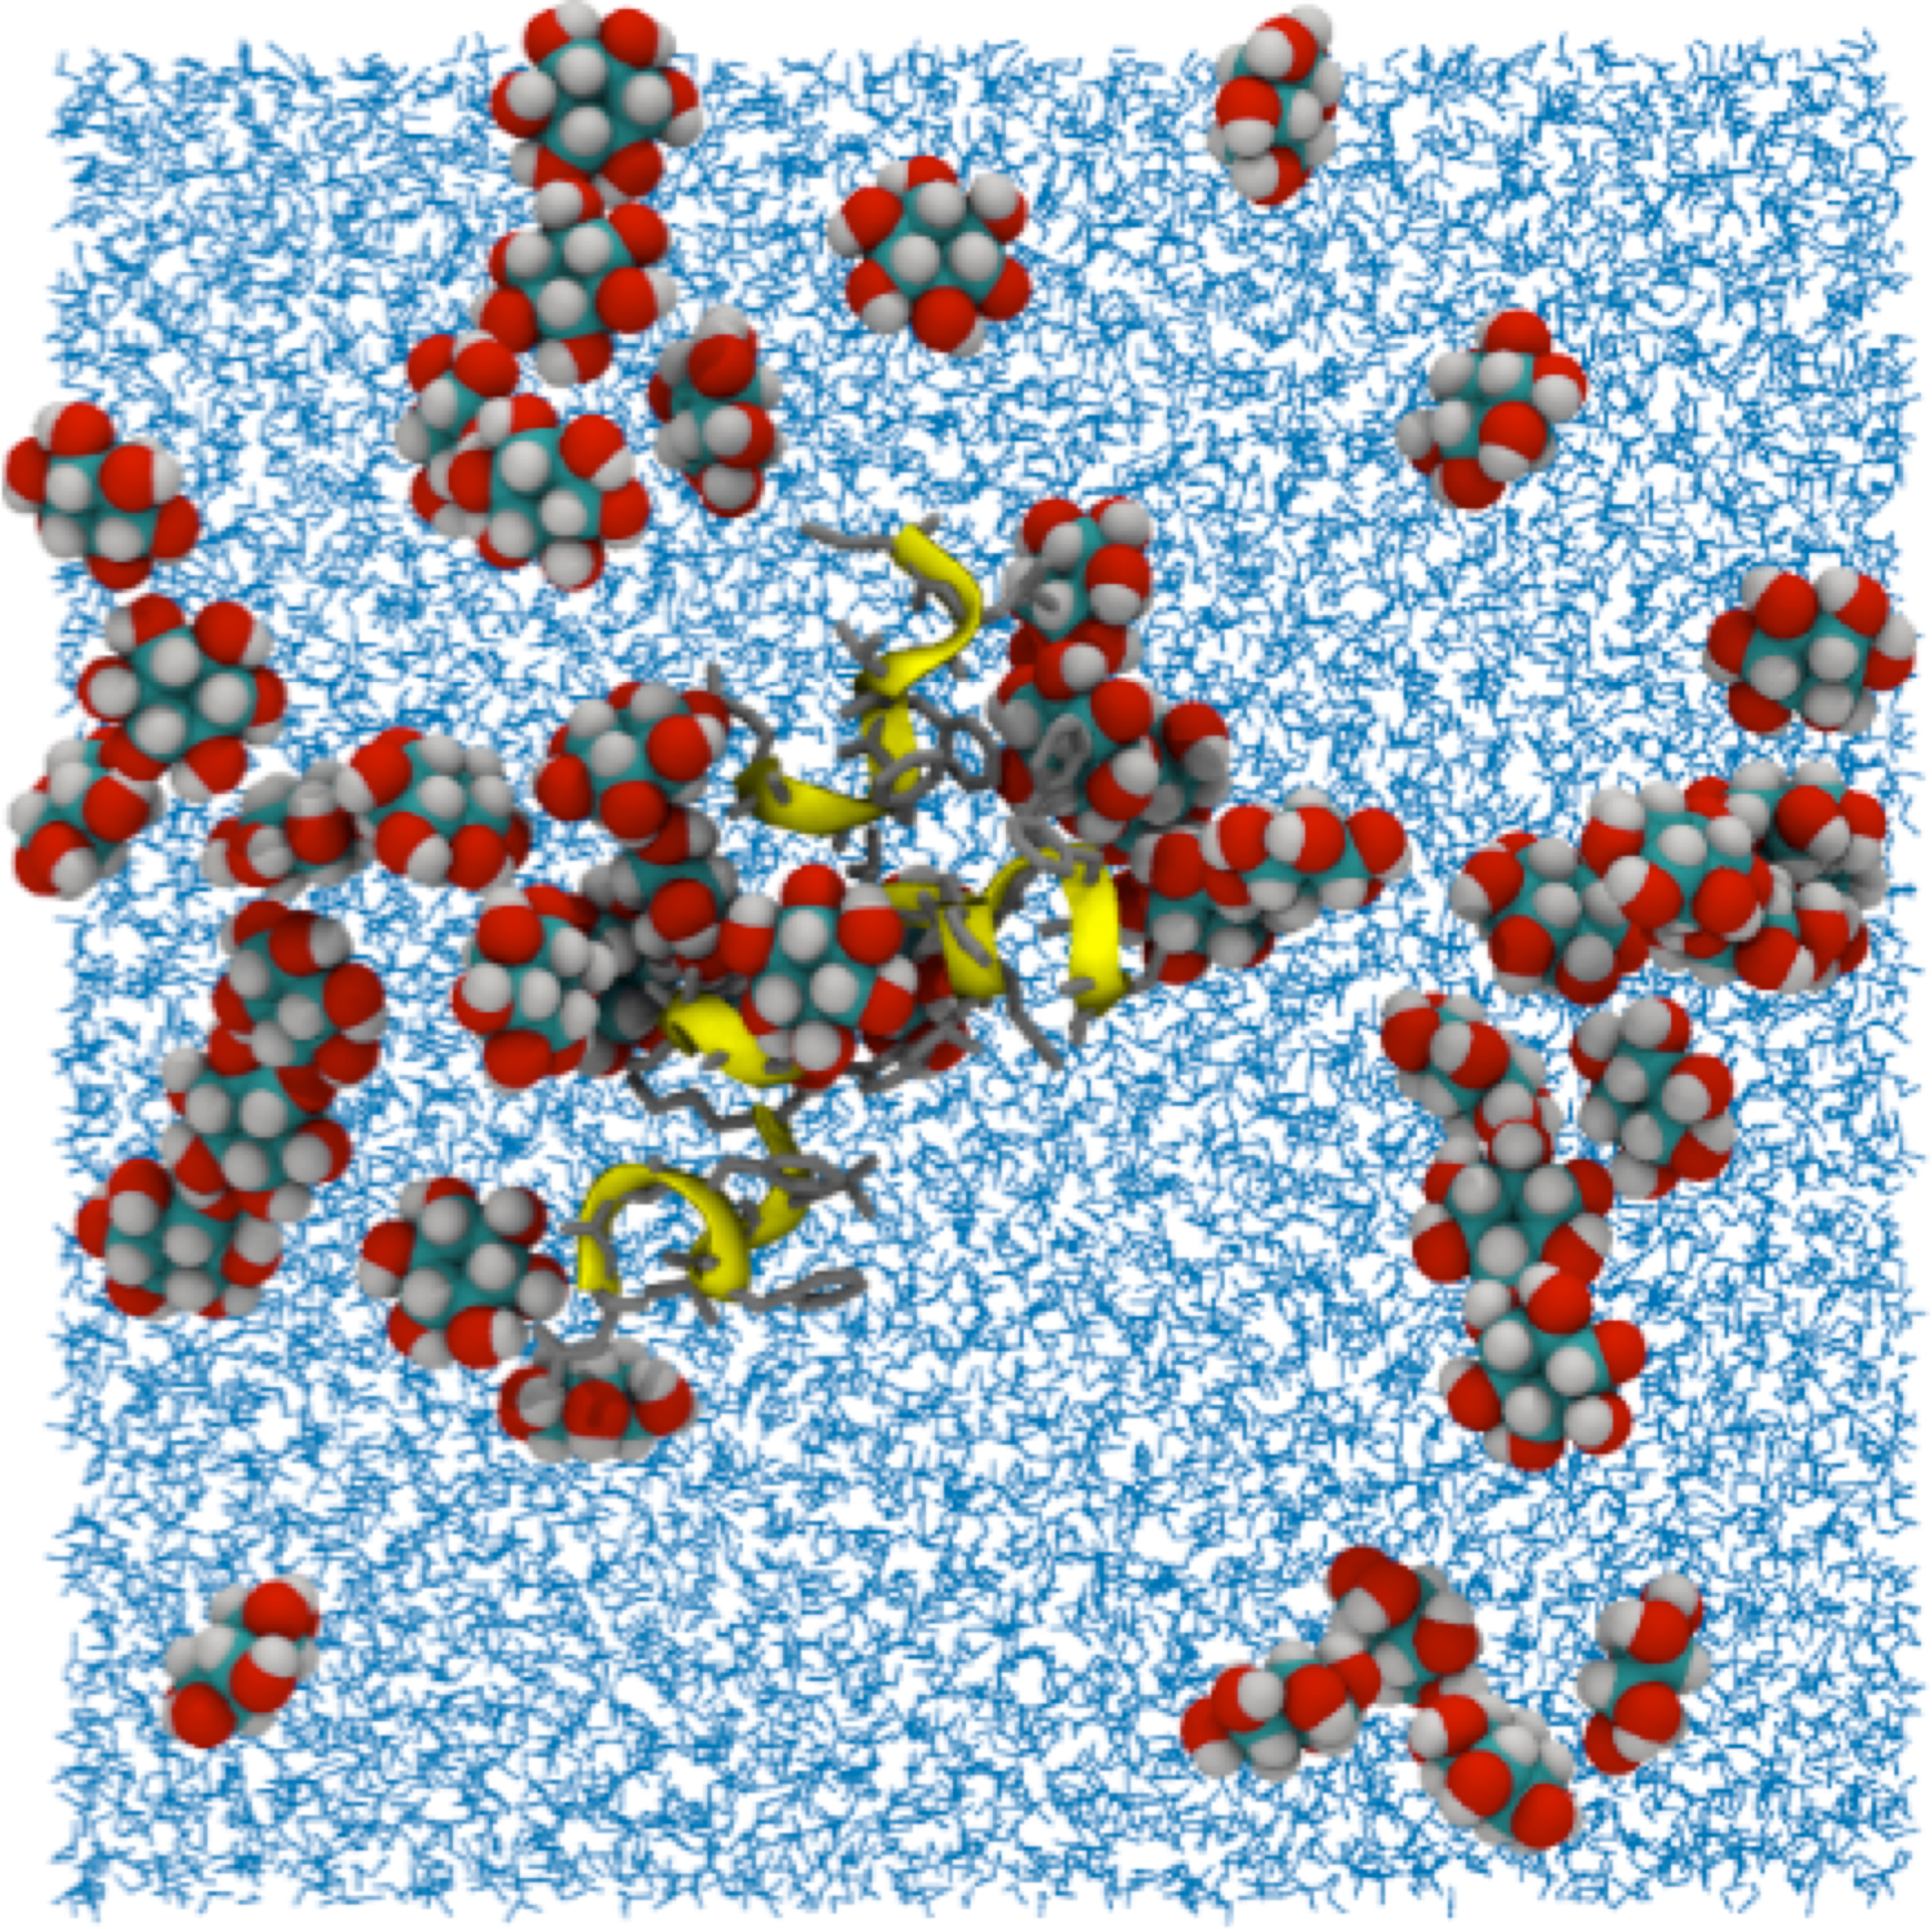
\includegraphics[width=5in]{figures/methods/simulation_box.pdf}
 \caption[An example of a MD simulation system]{An example of a MD simulation system.}
 \label{fig:simulation_box}
\end{figure}

Prior to performing production dynamics, which is what most of the results from a simulation will be based on, a short simulation to equilibrate the system is performed.  Equilibration is performed to allow the pressure and temperature of the system to stabilize. Here the stability of the protein is also validated to ensure that the protein structure has not grossly deviated (or unfolded) from the starting model.  

\begin{figure}
 \centering
 \includegraphics[width=5in]{figures/methods/equilibration.pdf}
 \caption[RMSD from the initial crystal structure calculated from an equilibriation]{Equilibration of the simulation system.}
 \label{fig:simulation_equilibration}
\end{figure}

\addcontentsline{toc}{section}{Bibliography}
\bibliographystyle{plain}
\bibliography{introduction}

%\section{Application of MD in structure-based drug discovery}
%
%% \1 (Why computational?) Can help us get protein dynamics is important for understanding protein function. We want to understand protein function because we want to be able to design drugs to cure diseases.
%
%% \1 A important application of MD simulation in biochemistry is the predicting of protein-ligand binding free energies.
%
%One application of MD simulations is in rational drug design. In recent years structure-based computer modeling of protein-ligand interactions have become a core component of modern drug discovery.  In early stage drug discovery, a target is identified along with putative binding sites.  Then, the structure of the target is determined using structural determination techniques such as NMR or X-ray crystallography.
%% [See Tom's thesis]
%Ligands which may act as potential drugs are expected to bind with a high affinity (low $K_d$) to the binding site. The goal is to discover,  high specificity inhibitors of a protein (usually an enzyme). In this process, the binding free energy of the ligand to its target is used to quantitatively evaluate how well a ligand binds. A crude estimate of the binding affinity can be obtained using computational docking methods, where the energetics of binding is typically estimated without accounting for either ligand or protein flexibility.  Although docking is fast, it is often inaccurate for identifying true drug candidates.
%
%With computer hardware becoming faster and cheaper, MD simulations can be used to rapidly prototype experimental ideas -- for example, one can perform computational alchemy, that is, ``mutate'' residues to test various hypotheses. Furthermore, simulations may be used to determine whether a chemical change will produce a more potent drug candidate. Currently, state of the art computational binding studies use MD simulations, where the protein and drug is allowed to relax and freely move about in the system. However, in the case of understanding a specific binding reaction often needed when developing an enzyme inhibitor, the ability to observe the relevant binding events is a low probability event on the timescale achievable by simulations. Therefore, a few enhanced techniques have been developed to accelerate this process.  They are briefly introduced below.
%
%\section{Free energy calculations}
%There are two advanced methods that have been developed for determining the absolute binding free energies in combination with MD simulations.
%
%% \3 Linear interaction energy -- Out of scope
%% \3 MM/PBSA - no explicit account for solvents -- Out of scope
%\subsection{Thermodynamic perturbation}
%This is the paper that I am taking most of the topics here\cite{Gilson:2007hz}
%
%\subsection{Thermodynamic integration}
%I actually have no idea what this is, and would be hard pressed to explain this properly.
%In this case, I don't think I should be covering these topics in my thesis.
%
%\subsection{Free energy perturbation}
%Alchemically change one molecule into another
%
%\section{Review of MD studies of amyloid inhibition by small molecules}
%% MD studies using brute-force sampling. Aid in medicinal chemistry by making suggestions for how to design new AD drugs.
%
%\begin{outline}
%	%  Excerpt from Transfer proposal
%	\1 In recent years, molecular dynamics simulations have been intensively used to investigate the molecular basis of the structure and stability of amyloid fibrils. 
%	
%	\1 MD simulations of Congo red binding have been done with the protofibril-like crystal structure composed of the segment GNNQQNY.\{Wu, 2007 \#621\}
%	
%	\1 A recent simulation study of an N-methylated peptide with A$\beta$16-22 models of amyloid aggregates has provided insight into the possible mechanism of action of peptide inhibitors of amyloid formation.\{Soto, 2007 \#597\} This peptide inhibitor was shown to preferentially bind monomers to form dimers, possibly acting to inhibit fibril formation by sequestering monomers. However, peptide-based inhibitors have poor pharmacological profiles as they are actively broken down by proteases in the stomach and are difficult to transport across the blood-brain barrier. In addition, these peptide inhibitors specifically target A$\beta$ and thus do not have the potential to treat multiple amyloid diseases.
%\end{outline}


% Scrap
% Motivate the use of MD simulations
% Describe the details of molecular dynamics simulations
% Review the basic derivations of MD simulation equations and why they work

% Molecular dynamics simulations are a useful tool to study the structure, dynamics, and interaction of biomolecules. 

% MD is a numerical algorithm which solves a system of Newtonian equations of motion, and provides as output the time-trajectory of atoms with femtosecond time resolution.

% To review before my defense

% Details of the mathematics (need to review the basic theory + Taylor series expansion) - get a book - tomorrow maybe?

% Why is MD correct? Describe the fundamental assumptions of MD. Here, I want to give the readers who aren't familiar with the methodological details of MD a sense of the rigorousness of MD.

% The assumption at a hand-wave level adapted from Tom's thesis

% - Relationship between force and energy 
% - Relationship between momentum and velocity 
% - Why numerical approach must be used (no analytical solution for N > 2)
% - How is the force field plugged into the general algorithm.






% \subsection{Setting up a MD simulation: practical aspects} - Here are some details to run a MD simulation of a biomolecular system.  Should I omit this from my introduction? This is not really essential in understanding the rest of my thesis, or is it? Perhaps this should go into an appendix instead -- this isn't interesting. The following steps are often used to setup and start a MD simulation system of a protein. First, a pre-determined structure, typically a coordinate structure from X-ray crystallography or NMR, or homology-modelling data. Then a force field and solvent is chosen.


%\section{Limitations of MD simulations}
% Rauscher:2010p5682,Rauscher:2009wr}  % Ref: DE Shaw and CN
% Schlick T (2010) Molecular modeling and simulation: an inter- disciplinary guide, interdisciplinary applied mathematics, vol 21, 2nd edn. Springer, New York


% Given the approximations of MD, MD is well-suited for probing the dynamics of complex systems on the timescale of picoseconds to seconds. ???

%Roughly speaking, one would like to run a simulation at least 10 times longer than the slowest important timescale in a system. Unfortunately, many biomolecular timescales exceed 1 ms, and in some cases by orders of magnitude (44).\cite{Zuckerman:2011dz} For molecular simulations to reliably predict, guide, and help explain experiment, these simulations require force fields of sufficient accuracy, adequate sampling of the relevant biomolecular motions (convergence) and a correct representation of the experimental conditions. Failures in any of these areas yield results which disagree with experiment.Until sampling is adequate, equilibrium properties computed from a simulation remain biased by the system�s starting state and no meaningful comparison with experiment is possible [6]. 

%% copied from Zukerman\cite{Zuckerman:2011dz}
%\textbf{Although routine explicit-solvent MD simula- tions are now four or five orders of magnitude longer (i.e., 100-103 ns currently), modern MD studies still appear to fall significantly short of what is needed for statistically valid equi- librium simulation (36, 38). Roughly speak- ing, one would like to run a simulation at least 10 times longer than the slowest impor- tant timescale in a system. Unfortunately, many biomolecular timescales exceed 1 ms, and in some cases by orders of magnitude (44).}
%% Other references that are relevant for sampling \cite{Grossfield:2009bn}
%
%% Copied from \cite{Mobley:2011ks}
%\textbf{For molecular simulations to reliably predict, guide, and help explain experiment, these simulations require force fields of sufficient accuracy, adequate sampling of the rel- evant biomolecular motions (convergence) and a correct representation of the experimental conditions. Failures in any of these areas yield results which disagree with experiment. 
%
%We may be tempted to blame disagreement with experiment on just one of these areas�force fields are perhaps the most common scapegoat, sometimes with good reason [1�5]�but any or all of the three may be a weak point. And, in some sense, adequate sampling is the weakest link. 
%
%Until sampling is adequate, equilibrium properties computed from a simulation remain biased by the system�s starting state and no meaningful comparison with experiment is possible [6]. 
%
%With an inadequate force field or a poor representation of the experimental conditions, results will disagree with experiment, but will be robust and improvement is relatively easy, but not so with inadequate sampling.}
%
%% copied from Sarah's thesis
%\textbf{Achieving complete (or even adequate) conformational sampling is one of the key challenges in biomolecular simulations.\cite{Gnanakaran:2003vh} The energy landscape of most biomolecules is �rugged� and the source of this ruggedness is two-fold. The energetic barriers separating accessible states are often larger than the available thermal energy, and there are typically a large number of states to be sampled. The timescales of many biomolecular processes, such as protein folding, are still far beyond the reach of our current computational capability, which is generally limited to the 10-8-10-7 s timescale for continuous simulations. For example, even the folding of small domains or secondary structure elements, such as ?-hairpins and mini-proteins, occur on the 1-10 ?s timescale.1 
%
%Consequently, conventional or �brute force� molecular dynamics (MD) alone is often insufficient to achieve complete Boltzmann sampling of the important states of many biologically relevant systems. For this reason, generalized-ensemble algorithms have become popular tools for conformational sampling.}

% Topics that I'm not going to discuss
%Evaluating the convergence of simulations is still a challenge - I don't want to  go into this as this is out of the scope of my thesis.
%Limitations in the accuracy of current force fields - Don't talk about this .. but this will probably come up during the defense regardless.
% \chapter{Binding of Inositol Stereoisomers to Model Peptides}

The contents of this section were adapted from an article published in the \emph{Journal of Physical Chemistry}.
\\
\\
\emph{Reference}:
Li, G., Rauscher, S., Baud, S., Pom\`{e}s, R. (2012). Binding of Inositol Stereoisomers To Model Amyloidogenic Peptides. Journal of Physical Chemistry B, 116(3), 1111–1119.
\\
\\
\emph{Contributions}:
Grace Li conducted the research and wrote the section. R\'{e}gis Pom\`{e}s provided editorial input and guidance.

\newpage

\section{Summary}
The self-aggregation of proteins into amyloid fibrils is a pathological hallmark of numerous incurable diseases such as Alzheimer's disease. \textit{Scyllo-}-inositol is a stereochemistry-dependent  \textit{in vitro}  inhibitor of amyloid formation. As the first step to elucidate its mechanism of action, we present molecular dynamics simulations of \textit{scyllo-}inositol and its inactive stereoisomer, \textit{chiro-}inositol, with simple peptide models, alanine dipeptide (ADP) and $(Gly-Ala)_4$. We characterize molecular interactions and compute equilibrium binding constants between inositol and ADP as well as, successively, monomers, amorphous aggregates, and fibril-like \bsheet\ aggregates of $(Gly-Ala)_4$.\cite{Balbach:2000p49}
Inositol interacts weakly with all peptide systems considered, with mM to M affinities, and displaces the conformational equilibria of ADP but not of the $(Gly-Ala)_4$ systems. However, \textit{scyllo-} and \textit{chiro-}inositol adopt different binding modes on the surface of \bsheet\ aggregates. These results suggest that inositol does not inhibit amyloid formation by breaking up preformed aggregates, but rather by binding to the surface of pre-fibrillar aggregates.

\section{Introduction}
Amyloid fibrils formed by various peptides and proteins are known to be associated with neurodegenerative diseases, type II diabetes, and prion-related disorders.\cite{Chiti:2006p20} In particular, amyloid fibrils of \abeta\ peptides are found in the extracellular deposits of neuronal plaques and are thought to be central to the pathogenesis of Alzheimer's Disease (AD),\cite{Chiti:2006p20,Hardy:2002p27} a common and incurable neurodegenerative disease causing dementia and eventual death. 

In recent years, amyloid fibril formation was discovered to be a common phenomenon among many proteins \textit{in vitro}; that is, under certain and denaturing conditions, proteins can self-aggregate to form amyloid fibrils.\cite{Chiti:2006p20} When viewed with negatively-stained transmission electron microscopy, amyloid fibrils appear as elongated, rope-like structures that are often 100 nm in length.\cite{Chiti:2006p20} The core structure of all amyloid fibrils is the cross-$\beta$-sheet.\cite{Chiti:2006p20,Serpell:2000p39} At the molecular level, NMR\cite{Balbach:2000p49,Petkova:2006p48} and X-ray crystallography\cite{Sawaya:2007p11} studies have revealed that the cross-$\beta$-structure is comprised of extended polypeptides organized in highly-ordered, in-register \bsheets. Although amyloid fibrils are a pathological hallmark of amyloid-based diseases, smaller nonfibrillar oligomers as little as three or four peptides in size have been demonstrated to display higher cytoxicity than mature fibrils.\cite{Gong:2003p22,Bitan:2003p10,Caughey:2009p5,Keshet:2010p61,Kitamura:2010p6,Lambert:1998p60,Selkoe:2008p16}

An important strategy to finding a cure to AD and other amyloid diseases is to derive new therapeutic candidates through the rational design of effective small-molecule inhibitors of amyloid formation. In recent years, a number of small molecules capable of preventing aggregation and/or fibril formation have been discovered and have emerged as potential therapeutic approaches for protein misfolding diseases.\cite{Frid:2007p65,Hawkes:2009p9,LeVine:2009p38,Necula:2007p42,ScherzerAttali:2010p63,Sood:2009p14} Interestingly, many of these small molecules share common chemical structural features, such as aromaticity and the presence of multiple hydrogen-bonding groups.\cite{Ehrnhoefer:2008p8,Liu:2009p18,Liu:2005p7,Porat:2006p33} However, the molecular basis of the structure-activity relationship of these small molecules is not understood, thus hindering drug development efforts for amyloid-based diseases.

Recently, one such small molecule, \textit{scyllo-}inositol, has shown promise as a therapeutic for AD.\cite{McLaurin:2006p29,McLaurin:2000p64} \textit{Scyllo-}-inositol is one of nine stereoisomers that belongs to a class of cyclic polyols called cyclohexanehexols. Four stereoisomers, \textit{myo-}, \textit{epi-}, \textit{scyllo-} and \textit{chiro-}inositol (Figure~\ref{fig:figure1}) are physiologically active.\cite{Fisher:2002p62} \textit{Myo-}inositol, the most abundant stereoisomer, plays an important role in signal transduction as precursor of phospholipid headgroups: once phosphorylated, \textit{myo-}inositol phosphatides act as second messengers in intracellular signal transduction pathways.\cite{Fisher:2002p62} Importantly for its therapeutic potential, inositol readily crosses the blood-brain barrier. \textit{Myo-} and \textit{scyllo-}inositol are found in tissues of the human central nervous system (CNS), with approximate concentrations of 5 mM and 0.1 to 0.5 mM, respectively.\cite{Michaelis:1993p89} Accordingly, they are also important osmolytes in the CNS, where alterations in their concentration have been associated with neuropathological conditions.\cite{Fisher:2002p62,Michell:2008p4}
 
\begin{figure}[htbp]
  \centering
  \includegraphics[width=3.25in]{figures/results1/GA4_paper_figures_submitted-1}
  \caption[Inositol stereoisomers most commonly found in nature.]
   {Inositol stereoisomers most commonly found in nature. Stick figures of the stereoisomers were drawn using the ChemDraw software.}
   \label{fig:figure1}
\end{figure}

\textit{In vitro}, inositol stereoisomers stabilize nonfibrillar $\beta$-structure and prevent the formation of amyloid fibrils in a stereochemistry-dependent manner: \textit{scyllo-}, \textit{epi-} and \textit{myo-}inositol inhibit \abeta\ fibril formation, but not \textit{chiro-}inositol.\cite{McLaurin:2000p64,McLaurin:1998p176,Nitz:2008p13,Sun:2008p12,Townsend:2006p44} Moreover, \textit{scyllo-}inositol was also demonstrated to be the most effective stereosiomer in preventing and reversing AD-like symptoms in transgenic mice while reducing their brain plaque load.\cite{McLaurin:2006p29} Despite this progress, the molecular basis of amyloid inhibition by inositol is not understood. \textit{In vitro} studies suggest that inositol stereoisomers affects aggregation through direct interaction with \abeta\ peptides.\cite{McLaurin:1998p176,McLaurin:2000p64,Nitz:2008p13,Sun:2008p12} However, it is not known whether inositol acts on monomeric peptides, non-fibrillar oligomers, or fibrillar aggregates.

Some small molecule inhibitors, including the osmolytes glycerol and trimethylamine N-oxide (TMAO), are known to interfere with \textit{in vitro} aggregation of amyloidogenic peptides with different sequences,\cite{Scaramozzino:2006p69,Yang:1999p77,McLaurin:2000p76,Ehrnhoefer:2008p8,Dasilva:2010p25,Bieschke:2010p32} suggesting that generic interactions common to all amyloid-forming peptides and proteins may play a role in the inhibition of amyloid formation. Indeed, small organic osmolytes are hypothesized to modulate protein folding equilibria by interacting with the peptidic backbone, the chemical group common to all polypeptides.\cite{Street:2006p21,Hu:2010p46,Auton:2008p28} Accordingly, the role of backbone solvation in the modulation of protein folding\cite{Rose:2006p35,Auton:2008p28} and aggregation equilibria has recently been highlighted.\cite{Rauscher:2006p43} Furthermore, several studies have suggested that N-methylation of the backbone of amyloidogenic peptides can abolish the formation of amyloid fibrils by preventing intermolecular backbone hydrogen bonding.\cite{Takeda:2010p52,Soto:2007p171}

Experimental efforts to characterize the molecular interactions of small molecules with amyloid oligomers and fibrils are often impeded due to the non-crystalline, transient, and disordered nature of the aggregates involved. By contrast, molecular simulations are well-suited for studies of proteins involving disorder.\cite{Rauscher:2010p88} Although several molecular dynamics (MD) simulation studies have begun to examine the effect of small molecules on aggregation and fibril formation,\cite{Takeda:2010p34,Raman:2009p47,Lemkul:2010p23,Liu:2009p18} the role of backbone binding has not been considered systematically.

In this chapter, we present an MD simulation study of the interaction of inositol with simple model peptides to investigate its stereochemistry-dependent effect on amyloidogenic peptide aggregation and morphology. In a systematic approach, we first characterize the binding equilibria of \textit{myo-}, \textit{epi-}, \textit{scyllo-} and \textit{chiro-}inositol with alanine dipeptide, a model of the peptidic backbone. Next, to probe the stereochemistry-dependent effect of inositol binding on amyloid aggregation, we study the interaction of \textit{scyllo-} and \textit{chiro-}inositol, respectively active and inactive stereoisomers in \abeta\ amyloid inhibition, succcessively with monomer, disordered, and fibrillar aggregates of $(Gly-Ala)_4$ or \gafour. \gafour\ is one of the simplest and shortest amyloidogenic peptides that is known to adopt an extended \bsheet\ structure both synthetically,\cite{Rathore:2001p37} as a metallocopolymer,\cite{Vandermeulen:2006p15} and in nature, in crystalline domains of spider silks.\cite{Kenney:2002p45,Fossey:1991fk} The repetitiveness and simplicity of the peptide sequence allow us to achieve statistically-significant estimates of the binding equilibrium from conventional sampling methods while focusing on the effect of backbone interactions in polypeptide self-aggregation. 

\section{Methods}
\subsection{Simulation Parameters and Protocol}
Alanine dipeptide (ADP) was methylated at both the N- and C-terminii. The \gafour\ peptide was acetylated and amidated at the N- and C-termini, respectively. The peptides were built using PyMol\cite{Anonymous:2012p58} and modelled using the OPLS-AA/L force field\cite{Jorgensen:1996p19}. The extended OPLS-AA force field for carbohydrates\cite{Damm:1997p36} was used to model inositol stereoisomers and the TIP3P water model\cite{Jorgensen:1983p40} was used to represent the solvent. Versions 3.3.1 and 3.3.3 of the GROMACS software package\cite{VanDerSpoel:2005p56} were used to perform unrestrained all-atom MD simulations with the leap frog algorithm using an integration timestep of 2 femtoseconds. Unless otherwise noted, the following parameters were used for all simulations in this study. Electrostatic interactions were calculated using Particle Mesh Ewald (PME) summation with a grid size of 0.15 nm and a real-space cutoff of 1.45 nm.\cite{Essmann:1995p51} The Lennard-Jones potential was computed up to 1.3 nm and was switched to zero at 1.4 nm using the GROMACS switch function. The temperature and pressure were controlled at 300 K and at 1 atm using the Berendsen thermostat and pressure coupling scheme, respectively.\cite{Berendsen:1984p26} Covalent bonds involving hydrogens were constrained using the SHAKE algorithm.\cite{Ryckaert:1977p30} All resultant simulation systems were first subjected to energy minimization and equilibration with isotropic pressure coupling. Replicas of every system were generated with different random seeds for the choice of initial velocities. A trajectory frame was written to disk every picosecond and all frames were used in the final data analysis. Additional details of simulation setup and total sampling time for all systems performed in this study are listed in Table~\ref{tab:simulations}.
	
	% TODO Change the first column to be left-justified and resized ... HOW?
  \begin{table}\footnotesize
    \begin{center}
    \vspace{10pt}
      \begin{tabular}{| p{2.5cm} | *{7}{p{1.25cm}|}}
        \hline
        System & $N_{peptides}$ & $N_{inositol}$ & $c_{peptide}$ (mM) & $c_{Inositol}$ (mM) & $N_{replicas}$ & Time per replica ($\mu$s) & Total time ($\mu$s) \\
        \hline
        \hline
        alanine dipeptide & 1 & 0 & 61.5 & 0 & 5 & 0.1 & 0.5\\
        with \textit{myo-}, \textit{epi-}, \textit{chiro-} or \textit{scyllo}-inositol & 1 & 4 & 61.5 & 246 & 5 & 0.1 & 0.5 \\
        \hline
        \gafour\ monomer & 1 & 0 & 61.5 & 0 & 1117 & 0.005 & 5.585 \\
        with \textit{chiro-} or \textit{scyllo-}inositol & 1 & 2 & 61.5 & 123 & 1117 & 0.005 & 5.585 \\
        \hline
        \gafour\ disordered aggregate (preformed) & 4 & 0 & 246 & 0 & 5 & 0.1 & 0.5 \\
        with \textit{chiro-} or \textit{scyllo-}inositol & 4 & 2 & 246 & 123 & 5 & 0.08 & 0.4 \\
        \hline
        \gafour\ disordered aggregate (dispersed) & 4 & 0 & 246 & 0 & 5 & 0.1 & 0.5 \\
        with \textit{scyllo-} & 4 & 2 & 246 & 123 & 4 & 0.08 & 0.32 \\
        with \textit{chiro-} & 4 & 2 & 246 & 123 & 3 & 0.08 & 0.24 \\
        \hline
        \gafour\ fibrillar aggregate & 16 & 0 & 437 & 0 & 3 & 0.1 & 0.3 \\
        with \textit{chiro-} or \textit{scyllo-}inositol & 16 & 4 & 437 & 109 & 3 & 0.1 & 0.3 \\
        \hline
      \end{tabular}
      \caption{Summary of simulation systems.}
      \label{tab:simulations}
    \end{center}
  \end{table}

Five initial starting conformations of ADP were obtained by taking a frame every 20 ns from a 100-ns-long simulation of ADP in water. Sets of five independent simulations were carried out successively in the presence of \textit{myo-}, \textit{epi-}, \textit{chiro-} and \textit{scyllo-}inositol. The initial conformations of monomeric \gafour\ were taken from an ensemble of monomeric structures generated in water at 296 K by simulated tempering distributed replica sampling (STDR) from a previous study.\cite{Nikolic:2011p57} STDR is a generalized-ensemble simulation method developed in our laboratory, which allows each replica in the simulation to undergo a random walk in temperature to enhance conformational sampling.\cite{Rodinger:2006p78} The STDR algorithm and implementation are described elsewhere.\cite{Rauscher:2009p41} A representative set of 1117 structures were chosen from the STDR ensemble at 296 K such that the end-to-end distance probability distribution of this selected subset is similar to the distribution of the entire STDR ensemble of structures (about 12,000 structures in total). These conformations were then used as starting points for simulations at T = 300 K in the presence of two molecules of either \textit{scyllo-} or \textit{chiro-}inositol. A total of 5 $\mu$s of simulation time was generated for the monomeric systems with either \textit{scyllo-} or \textit{chiro-}inositol (Table~\ref{tab:simulations}). The initial peptide conformations of disordered oligomeric systems were either dispersed monomers drawn from the STDR ensemble at 296K or a preformed \bsheet\ oligomer of \gafour\ composed of four peptides.

The \gafour\ peptide in the extended conformation was constructed using PyMol and was used to create the fibril-like \bsheet\ model. An eight-stranded antiparallel \bsheet\ was constructed by first creating an antiparallel dimer of \gafour. The principal axis of the dimer was then aligned with the x-dimension of the box and translated along the y-axis to form a single 8-stranded \bsheet. Two of these 8-stranded sheets were stacked in parallel in a ``face-to-back" manner (with all Ala methyl groups facing up in the z direction) and placed in the simulation box such that the first strand at the edge of the \bsheets\ was hydrogen-bonded in-register to the nearest periodic image of the eighth strand. The fibril-like systems were first subjected to energy minimization and a 500 ps equilibration stage. Production simulations were performed in the NVT ensemble with final box dimensions of 4 nm x 3.8 nm x 4 nm. Three independent simulations of the \gafour\ fibril-like systems were performed for 100 ns each, successively in the presence and absence of \textit{scyllo-} and \textit{chiro-}inositol (see Table~\ref{tab:simulations}).

\subsection{Analysis Protocol}
The DSSP geometry criteria\cite{Kabsch:1983p31} were used to determine the presence of a hydrogen bond: (1) the distance between donor (D) and acceptor (A) atoms is less than 0.35 nm; (2) the distance between the hydrogen and A is less than 0.25 nm; and (3) the angle formed by D-H-A is greater than 120\mathdeg. Nonpolar contacts between inositol and peptide were defined by a separation between the center of mass of inositol and the C$_{\beta}$ atom of alanine less than 0.45 nm. The same cut-off was used to compute protein-protein nonpolar contacts between C$_{\beta}$ atoms. 

All of the dissociation constants for inositol were calculated based on the presence of intermolecular contacts as defined above. Then, assuming that the binding equilibrium of inositol is
	
% Equations used in the KLVFFAE paper                                                                                                                  
\begin{equation}
  \left[ Protein\cdot Inositol \right] 
  \rightleftharpoons 
  \left[ Protein \right]+\left[ Inositol \right]
\end{equation}
  
the dissociation constant is the equilibrium constant of this reaction and is given by 

\begin{equation}
  K_{d} = \frac{\left[ Protein \right]\left[ Inositol \right]}{\left[Protein \cdot Inositol\right]} = f_{ub} [inositol],
\end{equation}
 
where $f_{ub}$ is the fraction of unbound over bound peptide states.

The DSSP algorithm was used for the analysis of secondary structure of the disordered oligomer with N- and C-termini of the peptides excluded. The end-to-end distance for a \gafour\ peptide was calculated as the distance between C$_\alpha$ atoms of the N and C-terminus of the peptide. The spatial probability density of inositol is the average spatial occupancy of the atoms of inositol and was computed using the VolMap tool from the Visual Molecular Dynamics (VMD) software package. %XXX {humphrey, 1996 #143} 
The planar angle between inositol and the fibrillar model of \gafour\ was computed using the g\_sgangle program from GROMACS analysis tools. All planar angles were corrected to a value between 0\mathdeg\ and 90\mathdeg, using the rule $\alpha = f(\theta) = 180 - \theta$, if $\theta > 90$\mathdeg, otherwise, $f(\theta) = \theta$. The probability distribution of the planar angles, $P(\alpha)$, was determined for inositol molecules with atoms within 0.25 $nm$ of the fibril. Average nonpolar and hydrogen bonding contacts in disordered aggregates were computed using the last 70 $ns$ of each trajectory. Error bars were determined by computing the standard deviation of the averages obtained from trajectories of independent replicas. Block averaging was used whenever a single trajectory was available.

\section{Results}
Inositol was found to bind weakly and reversibly to all the peptidic systems considered in our simulations, allowing us to characterize binding equilibria from unbiased sampling.

% This is a table with footnotes and with the footnote rule removed
% It uses the minipage and I had to tweak the width of the page so that center can 
% properly align the table in the middle of the page.
\begin{table}\footnotesize
  \vspace{10pt}
  \begin{minipage}{15cm}
    \renewcommand{\thefootnote}{\thempfootnote}
    \renewcommand{\footnoterule}{}
    % \centering
      \begin{center}
    \begin{tabular}{| l | *{5}{ c |}}
       \hline
         System & \textit{Scyllo-}\footnote{Each dissociation constant is in units of mM. The standard error is shown within parentheses.} & \textit{Chiro-} \footnotemark[\value{mpfootnote}] & N$_{groups,ADP}$/N$_{groups}$ & \textit{Scyllo-} \footnote{K$_d$ in units of $mM$, estimated by scaling the K$_d$ of ADP by the ratio of the number of \\ peptide groups in ADP to the \gafour\ system} & \textit{Chiro-}\footnotemark[\value{mpfootnote}]\\
         \hline
         \hline
         alanine dipeptide & 1100 (100) & 1000 (100) & 1.00 & 1100 & 1000 \\ 
         \gafour\ monomer & 376 (10) & 362 (16) & 0.25 & 275 & 250 \\ 
         \gafour\ preformed & 85 (12) & 89 (8) & 0.06 & 69 & 63 \\ 
         \gafour\ dispersed & 87 (21) & 86 (10) & 0.06 & 69 & 63 \\ 
         \gafour\ fibrillar & 51 (3) & 36 (15) & 0.02 & 17 & 16 \\
         \hline
     \end{tabular}   
  \end{center}
  \end{minipage}
  \centering
  \caption{Summary of equilibrium dissociation constants (K$_d$) for each system in the study.}
    \label{tab:binding_constants}
  \end{table}


\subsection{Alanine dipeptide}
Inositol stereoisomers bound weakly and reversibly to alanine dipeptide with a molar \KD. A list of computed dissociation constants for each stereoisomer is shown in Table~\ref{tab:binding_constants}. Because all of the results for \textit{myo-} (1.0 $\pm$ 0.1 M), \textit{epi-} (1.2 $\pm$ 0.2 M), \textit{chiro-} (1.0 $\pm$ 0.1 M) and \textit{scyllo-}inositol (1.1 $\pm$ 0.1 M) were within error bars of one another, in this section we provide detailed descriptions and data only for \textit{scyllo-}inositol. A single molecule of \textit{scyllo-}inositol can bind the peptidic backbone in either monodentate or bidentate fashion, as defined by the number of hydrogen bonds between hydroxyl groups of inositol and peptide groups. At a concentration of 250 mM, \textit{scyllo-}inositol was bound in the monodentate and bidentate modes about 14 $\pm$ 1\% and 1.1 $\pm$ 0.1\% of the time, respectively. The dominant bidentate binding modes of \textit{scyllo-}inositol involved hydrogen bonds formed with the peptide main chain either in the mean plane of the inositol ring (Figure~\ref{fig:figure2}, panels I-III) or in a ``face-to-edge" fashion, where the mean plane of the inositol ring is perpendicular to the plane of the peptide groups (Figure~\ref{fig:figure2}A, panel IV).
	
\begin{figure}[htbp]
    \centering
    \includegraphics[width=6in]{figures/results1/GA4_paper_figures_submitted-2-rearranged}
    \caption[Binding of \textit{scyllo-}inositol to the backbone of alanine dipeptide.]
     {Binding of \textit{scyllo-}inositol to the backbone of alanine dipeptide. A) Main bidentate binding modes. Ramanchandran maps of the conformations of alanine dipeptide sampled in absence of inositol are shown as contours in green. ($\phi$,$\psi$) of alanine dipeptide conformers bound by inositol are shown on the map as red crosses. $\beta$-conformers (top panels) are bound by inositol through adjacent or non-adjacent (CO,NH) groups; Helical conformers (bottom panels) involve mostly (CO,CO) and (NH,NH) groups. B) Comparisons of the conformational equilibrium of alanine dipeptide for different inositol backbone-bound states.}
     \label{fig:figure2}
  \end{figure}
  
The Ramachandran map of ADP is characterized by four dominant basins representing the $\alpha$�-helical, polyproline II (PPII), and \bsheet\ conformations.\cite{Neale:2008p87} As shown in Figure~\ref{fig:figure2}A, bidentate-bound ADP adopts backbone dihedral angles that fall within the dominant basins on the ramachandran map, demonstrating that \textit{scyllo-}inositol is able to bind both helical and \bsheet\ conformations. Notably, the conformational equilibrium of ADP is shifted in favor of the $\beta$-conformer when \textit{scyllo-}inositol is bound to the peptide backbone in bidentate fashion (Figure~\ref{fig:figure2}B); in contrast, the relative populations of dominant conformers remained unchanged when inositol is unbound or bound in monodentate form. Taken together, our results show that although binding is weak, inositol may influence peptide conformations by binding to the peptidic backbone. In the next sections, we examine the binding of inositol to monomer and aggregates of a simple \bsheet\ forming peptide, \gafour.

\begin{figure}[htbp]
  \centering
  \includegraphics[width=5in]{figures/results1/GA4_paper_figures_submitted-3-rearranged}
  \caption[Binding of \textit{scyllo-}inositol to the monomer of (GA)$_4$.]{Binding of \textit{scyllo-}inositol to the monomer of (GA)$_4$. A) Representative snapshot of \textit{scyllo-}inositol forming three hydrogen bonds to a monomer of (GA)$_4$. B) Distribution of the fraction of bound \textit{scyllo-}inositol to polar and nonpolar groups of the monomer. C-D) Conformational equilibrium of (GA)$_4$ as measured by the peptide end-to-end distance distribution. The distributions are all within error bars of each other and are plotted separately by the number of hydrogen bonds for \textit{scyllo-} in C) and \textit{chiro-}inositol in D). For clarity, error is only shown for the Peed curve where $n$=1.}
   \label{fig:figure3}
\end{figure}

\subsection{\gafour\ peptide}
In this section, we characterize the binding modes and binding affinity of inositol systematically, first with a peptide monomer, and then with oligomeric and fibrillar aggregates of \gafour. Here we examine only the active and inactive stereoisomers \textit{scyllo-} and \textit{chiro-}inositol. A summary of the equilibrium binding constants computed for all \gafour\ systems is shown in Table~\ref{tab:binding_constants}.

\subsubsection{Monomer}
In its monomeric state in solution, \gafour\ is an intrinsically disordered peptide.\cite{Nikolic:2011p57} An example of \textit{scyllo-}inositol binding to a monomer is shown in Figure~\ref{fig:figure3}A. Similar to ADP, binding is weak: the computed dissociation constants were \KD$_{,chiro}$  $\approx$ 362 $\pm$ 16 mM and \KD$_{,scyllo}$  $\approx$ 376 $\pm$ 10 mM. Most bound states, 95\% for \textit{scyllo-}inositol and 94.4\% for \textit{chiro-}inositol, involved hydrogen bonds to the backbone (Figure~\ref{fig:figure3}B). At a concentration of 123 mM, inositol molecules formed a single hydrogen bond about 9\% of the time, whereas two or more hydrogen bonds were formed about 4 to 5\% of the time. In contrast, nonpolar contacts are less frequent and, alone, account for only 3\% of bound \textit{scyllo-} and \textit{chiro-}inositol (Figure~\ref{fig:figure3}B). In total, the peptide monomer is bound to at least one molecule of inositol approximately 25\% of the time, 23\% of the time with a inositol:peptide stoichiometry of 1:1 and only $\sim$2\% of the time with a 2:1 stoichiometry. Contrary to ADP, the presence of inositol did not have a significant effect on the conformational equilibrium of monomeric \gafour\ (Figure~\ref{fig:figure3}C-D).

\subsubsection{Disordered Oligomer}

\begin{figure}[htbp]
  \centering
  \includegraphics[width=6in]{figures/results1/GA4_paper_figures_submitted-4-rearranged}
  \caption[Binding of \textit{scyllo-}inositol to the disordered oligomer of \gafour.]{Binding of \textit{scyllo-}inositol to the disordered oligomer of \gafour. A) Snapshot of \textit{scyllo-}inositol simultaneously hydrogen bonding two peptides in a disordered \gafour\ aggregate. Hydrogen bonds to the backbone are drawn as red lines. B) Distribution of secondary structure content, as classified by the DSSP algorithm, for preformed and dispersed starting states of the oligomer. Hydrogen bonds to the backbone are drawn as red lines. C) Fraction of \textit{scyllo-}inositol interacting with the disordered oligomer via hydrogen bonds (HBs), nonpolar contacts, or both. The fractions for \textit{chiro-}inositol are similar (data not shown).}
   \label{fig:figure4}
\end{figure}

To probe whether inositol affects the structure and aggregation of small oligomers of \gafour\ in solution, we performed sets of simulations involving two distinct starting states of four \gafour\ peptides: (1) initially monodispersed peptides and (2) a preformed \bsheet\ aggregate. In the initially dispersed systems, the peptides rapidly aggregated to form a disordered oligomer (Figure~\ref{fig:figure4}A) in which the majority of the residues ($\sim$60\%) retained a coil conformation (Figure~\ref{fig:figure4}B). Similarly, systems initiated with a preformed 4-stranded \bsheet\ also evolved into a disordered oligomer over the course of the simulation. Only about 5\% and 10\% of the residues participated in a \bsheet\ or in a \bbridge, respectively (Figure~\ref{fig:figure4}B).
	
\begin{figure}[htbp]
  \centering
  \includegraphics[width=4.5in]{figures/results1/GA4_paper_figures_submitted-5}
  \caption[Time evolution of peptide-peptide nonpolar and hydrogen bonding contacts in disordered aggregates in presence and absence of inositol (control).]{Time evolution of peptide-peptide nonpolar and hydrogen bonding contacts in disordered aggregates in presence and absence of inositol (control). Each curve is smoothed using a running average over a window with a length of 500 ps. Results for the dispersed monomer aggregates are shown on the left and the preformed $\beta$-sheet aggregates on the right. Top: the total number of inter- and intra-molecular hydrogen bonding contacts; Bottom: Number of intermolecular nonpolar contacts.}
   \label{fig:figure5}
\end{figure}
  
Despite different initial conditions and independently of the presence of inositol, all aggregates evolved to a similar morphology. The total number of peptide-peptide nonpolar and polar contacts formed within the oligomer converged to similar values for both the dispersed and preformed oligomers and did not change with time (Figure~\ref{fig:figure5}). As shown in Figure~\ref{fig:figure5} (top panels), the average total number of intermolecular hydrogen bonds ($\sim$8 $\pm$ 1) was consistently higher than the number of intramolecular hydrogen bonds ($\sim$2.1 $\pm$ 0.3). On average, about 4.3 $\pm$ 0.4 nonpolar contacts were formed upon aggregation in the absence of inositol compared to 4.4 $\pm$ 0.5 contacts for \textit{scyllo-}, and 5.0 $\pm$ 0.4 for \textit{chiro-}inositol (data not shown for the preformed oligomer). When taken together, the above results show that the presence of \textit{scyllo-} and \textit{chiro-}inositol neither prevented aggregation nor disrupted the preformed oligomer.

Dissociation constants of about 80 mM to aggregates of type 1 and 2 were obtained for both \textit{scyllo-} and \textit{chiro-}inositol. The \KD\  calculated for each aggregate type is shown in Table~\ref{tab:binding_constants}. In the presence of multiple aggregated chains, a single molecule of inositol was found to cross-link multiple peptides by simultaneously hydrogen bonding to their backbones (Figure~\ref{fig:figure4}A). Similar to monomers, at a concentration of 123 mM, \textit{chiro-} and \textit{scyllo-}inositol were bound predominantly to the backbone: ~96\% of bound \textit{scyllo-}inositols formed only hydrogen bonding contacts ($\sim$94\% for \textit{chiro-}inositol), whereas 2\% (3\% for \textit{chiro-}inositol) were involved in nonpolar contacts only (Figure~\ref{fig:figure4}C).

\subsubsection{Fibril-like oligomer} % (fold)

\begin{figure}[htbp]
  \centering
  \includegraphics[scale=0.75]{figures/results1/GA4_paper_figures_submitted-6}
  \caption[Binding of \textit{scyllo-} and \textit{chiro-}inositol to the fibrillar aggregate of \gafour.]{Binding of \textit{scyllo-} and \textit{chiro-}inositol to the fibrillar aggregate of \gafour. Different views of the initial starting structure of the fibril-like model. Top and bottom sheets are colored in grey and in cyan, respectively. A top down view is depicted in A) showing the backside of the top \gafour\ sheet. A side view of the protofibril is shown in B). The spatial probability density of bound \textit{scyllo-}inositol (yellow) C) and \textit{chiro-}inositol (orange) D) are shown overlapping with the fibril. The density is shown at an occupancy isosurface value of 3\% for both stereoisomers. E) is the percentage of bound \textit{scyllo-} and \textit{chiro-}inositol to polar and nonpolar groups on the \bsheet.}
   \label{fig:figure6}
\end{figure}

In order to probe the binding modes of inositol with a fibril-like aggregate of \gafour, we constructed an ‘infinite \bsheet’, where the $\beta$-strands at the edge of an octameric \bsheet\ are hydrogen-bonded to each other’s nearest periodic image. A single unit of this periodic model consisted of a stack of two antiparallel and in-register \bsheets, with eight strands per sheet (Figure~\ref{fig:figure6}A,B). Although some of the hydrogen bonds defining the \bsheet\ structure occasionally broke, in the absence of inositol the protofibril remained approximately planar and aggregated as an infinite fibril throughout the simulation.

The spatial distribution of bound inositol molecules shows that both \textit{chiro-} and \textit{scyllo-}inositol bind at the surface of the fibril (Figures~\ref{fig:figure6}C, D). \textit{Chiro}- and \textit{scyllo-}inositol bound fibrillar aggregates of \gafour\ with a \KD\ of 36 $\pm$ 15 mM and 51 $\pm$ 3 mM, respectively. The apparent increase in affinity compared to amorphous aggregates can be attributed to the following reasons. First, the fibrillar aggregate presents a much larger effective surface area than both the monomer and the disordered oligomer (Figures~\ref{fig:figure6}C, D). Moreover, a larger fraction of the alanine side chains are completely solvent-exposed in the fibril-like aggregate, increasing the fraction of bound conformations involving only nonpolar contacts by nearly an order of magnitude, from 2\% in the disordered oligomer to 12\% for \textit{scyllo-} and 18\% for \textit{chiro-}inositol in the fibrillar aggregate in the presence of 109 mM of inositol (Figures~\ref{fig:figure3}B and \ref{fig:figure6}E). Accordingly, a higher fraction of \textit{scyllo-}inositol, 83 $\pm$ 1\%, versus 77 $\pm$ 1\% for \textit{chiro-}inositol, was found to form hydrogen bonds, where the 6\% drop in the hydrogen-bonded-only population of \textit{chiro-}inositol was compensated by a commensurate increase in the nonpolar-bound-only population of \textit{chiro-}inositol (Figure~\ref{fig:figure6}E).

\begin{figure}[htbp]
  \centering
  \includegraphics[width=3.2in]{figures/results1/GA4_paper_figures_submitted-7}
  \caption[Example snapshots of \textit{scyllo-} and \textit{chiro-}inositol binding to the fibril of \gafour.]{Example snapshots of \textit{scyllo-} and \textit{chiro-}inositol binding to the fibril of \gafour. Red and blue dashed lines denote hydrogen bonds. A-B) Example binding modes of \textit{scyllo-} and \textit{chiro-}inositol binding at an angle to the surface. C-D) Example binding modes of \textit{scyllo-} and \textit{chiro-}inositol binding face down on the sheet.}
   \label{fig:figure7}
\end{figure}

Thus, although \textit{chiro-} and \textit{scyllo-}inositol have similar binding constants, they have different binding modes to fibrillar aggregates, a feature not previously observed for the monomer and the disordered oligomer of \gafour. Both \textit{scyllo-} and \textit{chiro-}inositol form nonpolar contacts and backbone hydrogen bonds in poses where the mean plane of the inositol ring lies parallel, at an angle, or perpendicular to the plane of the fibril (Figure~\ref{fig:figure7}). Furthermore, two or more molecules of inositol may cluster together and bind at the surface of the sheet (Figures~\ref{fig:figure7}C,D). However, as shown in Figure~\ref{fig:figure8}A, \textit{scyllo-}inositol adopts specific binding orientations whereas \textit{chiro-}inositol does not: \textit{scyllo-} preferentially binds in either nearly flat ($\alpha = 20$\mathdeg) or upright ($\alpha = 65$\mathdeg) to the sheet, whereas \textit{chiro-}inositol does not have such a bimodal preference and binds the fibril at an average angle of $\alpha = 45$\mathdeg. This stereochemistry-modulated difference in binding specificity explains the somewhat higher fraction of nonpolar binding by \textit{chiro-}inositol (Figure~\ref{fig:figure6}E): \textit{chiro-} is more likely than \textit{scyllo-}inositol to bind at angles of $30$\mathdeg $< \alpha \leq 60$\mathdeg (Figure~\ref{fig:figure8}A), where 24\% of bound \textit{chiro-} (versus 16\% for \textit{scyllo-}inositol) is bound by nonpolar contacts only (Figure~\ref{fig:figure8}B). For $\alpha \leq 30$\mathdeg, the distributions of \textit{scyllo-} and \textit{chiro-}inositol bound to polar and nonpolar groups are similar (data not shown). Moreover, because \textit{chiro-}inositol has a partially-nonpolar edge whereas \textit{scyllo-}inositol does not, binding in the upright position also involves more nonpolar interactions for \textit{chiro-} than for \textit{scyllo-}inositol (Figure~\ref{fig:figure8}B). Finally, although inositol was observed to bind at the surface, binding did not change the morphology of the fibrillar aggregate.

\begin{figure}[htbp]
  \centering
  \includegraphics[width=6in]{figures/results1/GA4_paper_figures_submitted-8-rearranged}
  \caption[Binding mode and orientation of \textit{scyllo-} and \textit{chiro-}inositol to the fibril of \gafour.]{Binding mode and orientation of \textit{scyllo-} and \textit{chiro-}inositol to the fibril of \gafour. The distribution of inositol to sheet planar angles is depicted in A). B) Inositol binding to nonpolar and polar groups as classified by $\alpha$, the angle at which inositol molecules bind at the surface of the fibrillar \gafour\ (see Methods).}
   \label{fig:figure8}
\end{figure}

\section{Discussion}
In the above analysis, we have systematically characterized the association of stereoisomers \textit{scyllo-}, \textit{epi-}, \textit{myo-} and \textit{chiro-}inositol with alanine dipeptide, a simple model of the peptidic backbone. Furthermore, we examined the binding of \textit{scyllo-} and \textit{chiro-}inositol to various aggregated states of \gafour\ to probe the role of backbone binding in amyloid inhibition. Our results show that inositol exhibits weak binding with dissociation constants in the range of 0.04 M to 1 M to the different peptides and aggregation states considered.

Furthermore, the \KD\ of inositol increases linearly with the number of peptide groups in the system (Table~\ref{tab:binding_constants}), indicating that inositol does not bind cooperatively to the monomer and aggregate states of \gafour\ considered. As expected, inositol binds most weakly to alanine dipeptide, with a value about 4 times smaller than the \KD\ of urea to N-acetyl alanine reported recently in the literature (0.3 M for urea\cite{Lee:2010p59} vs 1.1 M for \textit{scyllo-}inositol). Taken together, our results indicate that the activity of inositol stereoisomers is similar to that of osmolytes, which typically have binding constants in the millimolar to molar range.\cite{Rosgen:2007p90,Street:2006p21}

Moreover, our results are consistent with the hypothesis that osmolytes influence protein and peptide folding and stability through direct binding rather than by modifying solvent properties.\cite{Canchi:2011p53,Lee:2010p59,Street:2006p21} The spacing of consecutive OH groups of inositol is well-suited to bidentate interactions with adjacent groups of the polypeptide backbone (Figure~\ref{fig:figure2}A). Our findings shown in Figure~\ref{fig:figure2}A are consistent with similar binding modes observed in a recent ab initio simulation and IR spectroscopic study of the binding of glucose epimers to the phenylalanine dipeptide backbone.\cite{Cocinero:2011p54} Furthermore, inositol stereoisomers displace the backbone conformation of alanine dipeptide towards extended $\beta$-strand conformations (Figure~\ref{fig:figure2}B). However, neither \textit{scyllo-} nor \textit{chiro-}inositol had a significant effect on the conformational equilibrium of the \gafour\ monomer. Taken together, these results indicate that inositol may not act as a drug by directly influencing monomer conformations. However, our results do not preclude the possibility that inositol may block fibril elongation by preferentially binding to monomers that are constrained to extended conformations, such as those at exposed edges of \bsheets.

Independently of the presence of inositol, both the preformed \bsheet\ oligomer and the monodisperse solution of \gafour\ evolved into a similar morphology (Figure~\ref{fig:figure4}B and \ref{fig:figure5}) with only a small amount of $\beta$-structure (Figure~\ref{fig:figure4}B), indicating that small aggregates of \gafour\ are likely to be disordered. Unlike the hydrophobic core of the \abeta\ peptide, \gafour\ is a shorter and more polar peptide that is capable of forming more hydrogen bonds than nonpolar contacts. Our results show that peptide-peptide hydrogen bonding play an important role in the aggregation of \gafour\ peptides in solution (Figure~\ref{fig:figure5}). Because neither stereoisomer disrupted the aggregates of \gafour, our results indicate that inositol is unlikely to inhibit fibril formation by breaking up preformed aggregates. Therefore, we conclude that inositol is unlikely to inhibit fibril formation by binding monomers and small disordered oligomers since binding appears to be weak, non-cooperative, and stereochemistry-independent.

By contrast, although the dissociation constants were similar for both \textit{scyllo-} and \textit{chiro-}inositol, binding specificity and binding modes involving nonpolar groups of the fibrillar aggregate of \gafour\ were modulated by the stereochemistry of inositol. A significantly higher fraction of \textit{chiro-}inositol than \textit{scyllo-}inositol was bound to nonpolar groups of the fibrillar aggregate (Figure~\ref{fig:figure6}E). Moreover, \textit{scyllo-}inositol exhibited a bimodal distribution of binding orientations, with a significant preference for orientations in which the ring of inositol is either parallel or perpendicular to the mean surface of the \bsheet\ over \textit{chiro-}inositol (Figure~\ref{fig:figure7}). As a direct consequence of the presence of axial hydroxyl groups, \textit{chiro-}inositol is more likely to bind at angles that promote contact with nonpolar groups at the surface of the fibrillar aggregate, whereas the more specific binding modes of \textit{scyllo-}inositol favors backbone binding. Since this is the only stereochemistry-dependent result of our study, we speculate that \textit{scyllo-}inositol acts on ordered \bsheet\ aggregates (as opposed to disordered oligomers or monomers). Moreover, these findings suggest a possible mechanism of action whereby a significant binding affinity to specific side chains on the surface of fibrillar aggregates could lead to the inhibition of \bsheet\ stacking (and therefore, amyloid fibril growth or maturation) by \textit{scyllo-}inositol. Similarly, different binding modes observed in MD simulations of \abeta42 fibrils have been proposed to explain differences in binding affinities between Thioflavin T, a well-known amyloid-binding dye, and its chemical analogs.\cite{Mathis:2003p55,Wu:2011p24}

A factor that we have not considered in this study is the influence of inositol:peptide molar ratio on binding and inhibition. \textit{In vitro}, the inhibition activity of \textit{scyllo-}inositol was observed at an inositol:peptide ratio of 25:1, where inositol stereoisomers were present in excess of \abeta\ at concentrations of 0.25 mM to 5 mM.\cite{McLaurin:2000p64} Although our simulations had effective concentration of inositol an order of magnitude higher than in these experiments, it is possible that we have precluded cooperative inositol binding modes by limiting the number of inositol molecules present in the small simulation cell. Furthermore, \KD\ values obtained from our simulations of \gafour\ were approximately two orders of magnitude higher than measured for \abeta. Based on our results, the predicted \KD\ of (GA)$_{21}$, a Gly-Ala repeat peptide similar in length to \abeta, would be 1200 mM/21 = 57 mM, which is still an order of magnitude greater than \textit{in vitro} inhibitory concentrations. This indicates that \textit{scyllo-}inositol is unlikely to inhibit \bsheet\ formation by \gafour\ peptides, and more importantly, that backbone binding by small molecules may not be sufficient for inhibition of amyloid formation. In future studies, elucidating the relationship of binding cooperativity and amyloid inhibition by approaching experimental drug:protein molar ratios, as well as elucidating the sequence specificity of inositol binding to amyloid fibrils, will provide further insight that may be used in the rational drug design of improved inhibitors.

\section{Conclusions}
We have performed systematic simulations of simple amyloidogenic peptide models with both active and inactive stereoisomers of inositol to examine the molecular basis of amyloid inhibition. Our results indicate that although peptide backbone dominates the interaction with inositol, the binding affinity is low and remains in the millimolar range. Moreover, this property is independent of stereochemistry and does not appear to be sufficient to impede peptide dimerization through intermolecular backbone hydrogen bonding. Taken together, our results suggest that amyloid inhibition by inositol cannot be accounted for by generic binding to the peptidic backbone alone and is likely to involve sequence-specific interactions with amino-acid side chains as well as binding to specific aggregate morphologies. Accordingly, although the formation of intermolecular hydrogen bonds is the predominant interaction in protein aggregates composed of \gafour, amyloidogenic peptides involved in amyloid diseases are often more hydrophobic and in general, self-aggregation is driven largely by the hydrophobic effect.\cite{Chiti:2006p20} In forthcoming studies, we will examine the role of sequence-specific interactions between inositol and aggregates of pathogenic peptides.


\begin{singlespace}
\addcontentsline{toc}{section}{Bibliography}
\bibliographystyle{elsart-num}
\bibliography{results1/results1}
\end{singlespace}

% \chapter{Binding of inositol to monomers and aggregates of A$\beta$(16-22)}

% The contents of this section were adapted from an article published in the \emph{Journal of Physical Chemistry}.
% \\
% \\
% \emph{Reference}:
% Li, G., Rauscher, S., Baud, S., & Pomès, R. (2012). Binding of Inositol Stereoisomers To Model Amyloidogenic Peptides. Journal of Physical Chemistry B, 116(3), 1111–1119.
% \\
% \\
\emph{Contributions}:
Grace Li conducted the research and wrote the section. Régis Pomès provided editorial input and guidance.

\section{Summary}
	Alzheimer's disease (AD) is a severe neurodegenerative disease with no cure. Currently, one method of targeting the underlying disease is to prevent or reverse the amyloid formation of A$\beta$42, a key pathological hallmark of AD. Scyllo-inositol is a polyol that exhibits stereochemistry-dependent inhibition of the formation of A$\beta$ fibrils \emph{in vitro}. We present molecular dynamics simulations of the monomeric, disordered and protofibrillar states of A$\beta$(16-22), an amyloid-forming peptide fragment found in the $\beta$-sheet core of full-length A$\beta$, successively with and without \emph{scyllo}-inositol and its inactive stereoisomer \emph{chiro}-inositol. Inositol binds monomers and disordered aggregates of A$\beta$(16-22) with similar affinities, whereas binding to $\beta$-sheet containing oligomers ($\beta$-oligomers) yield affinities in the low millimolar range commensurate with \emph{\emph{in vitro}} inhibitory concentrations of inositol. Furthermore, inositol adopts carbohydrate-like binding modes, where stereochemistry modulates the nonpolar binding specificity of inositol to glutamate and phenylalanine side chains. Our results suggest that \emph{scyllo}-inositol inhibits amyloid formation by coating the surface of protofibrillar aggregates of A$\beta$ and disrupting their lateral stacking into fibrils.


\section{Introduction}

One in eight people over the age of 65 has Alzheimer's Disease (AD), a progressive neurodegenerative disease that currently has no cure.\cite{Citron:2010p214} The amyloid cascade hypothesis states that the extracellular neuronal deposition of A$\beta$ amyloid plaque plays a central role in the pathogensis of AD.\cite{Solomon:2010p177} A$\beta$ is a peptide proteolytically cleaved from the amyloid precursor protein (APP) and is produced as two common alloforms, A$\beta$40 or A$\beta$42, which are 40 and 42 residues in lengths, respectively. In the diseased state, A$\beta$42 levels are elevated, and the peptides deposit as extracellular A$\beta$ plaques.\cite{Haass:2007p226,Citron:1997p228}

A$\beta$40 and A$\beta$42 are intrinsically disordered peptides that self-aggregate \emph{in vitro} to form amyloid fibrils. Amyloid fibrils are protein aggregates with a characteristic cross-$\beta$ structure, which consists of in-register $\beta$-sheets with backbone hydrogen bonds running parallel to the long axis of the fibril.\cite{Petkova:2002p192} Moreover, smaller fragments of the full length A$\beta$ sequence are also found to form amyloid in vitro.\cite{Balbach:2000p49,Sawaya:2007p11} In particular, one of the shortest amyloid-forming peptides structurally characterized using solid-state NMR is KLVFFAE or A$\beta$(16-22).\cite{Balbach:2000p49} The residues LVFFA are believed to form the central hydrophobic core critical for the initiation of aggregation and fibril formation in the full length A$\beta$ peptide.\cite{Wood:1995p190} Furthermore, single-point mutations in this region greatly affect the aggregation propensity of A$\beta$: known familial mutations E22Q, E22K, and E22G, known as ``Dutch'', ``Italian'' and ``Arctic'' mutations, respectively, significantly accelerate fibril formation,\cite{Kim:2008ef} whereas the mutation F19T abolishes the formation of fibrils \emph{in vitro}.\cite{Esler:1996p288}

% check the different mutations, might be missing one
% TODO use more connectives to draw the links between the concepts introduced

Amyloid fibril formation follows a complex pathway: Prior to the appearance of fibrils in vitro, amyloidogenic monomers self-aggregate into a variety of pre-fibrillar intermediate morphologies. While the fibril is an important state implicated in AD, recent research has shown that soluble oligomers as small as dimers and tetramers play a role in neurotoxicity.\cite{Bernstein:2009p165} In recent years, drug development and research efforts have been directed towards the development of therapeutic agents to prevent the self-aggregation and amyloid formation of A$\beta$, a promising treatment approach to target the underlying disease.\cite{Masters:2006p183,Citron:2010p214,Dasilva:2010p25} As a result, many different types of \emph{in vitro} amyloid inhibitors have been discovered, including peptide molecules,\cite{EsterasChopo:2008p219,Sciarretta:2006p181,Chalifour:2003p161,Scrocchi:2002p178} immunotherapies,\cite{Janus:2000p198,Solomon:2010p177} polyphenolic molecules,\cite{Masuda:2009p205,Berhanu:2010p230,Ehrnhoefer:2008p8} and other small molecules.\cite{Hawkes:2009p189,Masuda:2009p205,Necula:2007p227,Nitz:2008p13} These approaches have been reviewed in detail elsewhere.\cite{Citron:2010p214,Dasilva:2010p25} 
% Despite experimental progress made in recent years, still lack a mechanistic understanding how these small molecules work. These approaches have been reviewed in detail elsewhere.\cite{Citron:2010p214,Dasilva:2010p25}

\emph{scyllo}-Inositol is a small-molecule A$\beta$ amyloid inhibitor developed for the treatment of AD.\cite{Dasilva:2010p25,Hawkes:2009p189,McLaurin:2000p64,Nitz:2008p13,Sun:2008p208} Inositol is a class of polyols, of which eight out of nine stereoisomers are commonly found in nature (Fig. 1). \emph{Myo}-inositol, the most common isomer, is found at high concentrations in the tissues of the human central nervous system (CNS).\cite{Fisher:2002p62} Like \emph{myo}-inositol, \emph{scyllo}-inositol is also present in the brain and can be passively and actively transported across the blood-brain barrier.\cite{Fenili:2007p182} Importantly, \emph{scyllo}-inositol was demonstrated to prevent and reverse AD-like symptoms in a transgenic mouse model of AD.\cite{McLaurin:2006p29} Because of the positive CNS bioavailability and favorable \emph{in vivo} toxicity profile of inositol, both of which are rare and essential properties of putative AD drug candidates, inositol-based therapies represent unique and promising approach for the treatment of AD. In 2007, \emph{scyllo}-inositol (ELN0005) was fast-tracked by the United States Food and Drug Administration into phase II of clinical trials in North America.

\emph{In vitro}, inositol displays stereochemistry-dependent inhibition of A$\beta$42 fibrils: \emph{myo}-, \emph{epi}- and \emph{scyllo}-inositol were shown to inhibit A$\beta$42 fibrillation at concentrations of 1 - 5 mM,\cite{McLaurin:2000p64} whereas \emph{chiro}-inositol is inactive below molar concentrations.\cite{Janus:2000p198} Moreover, upon incubation of monomeric A$\beta$42 with \emph{scyllo}-inositol, circular dichroism spectroscopy indicated the formation of $\beta$-sheet structure at an inositol:peptide molar ratio of 25:1.\cite{McLaurin:1998p176} Although inositol stereoisomers have been proposed to inhibit amyloid formation by directly interacting with either monomers or non-fibrillar aggregates to ``cap off'' fibril growth,\cite{Janus:2000p198} the molecular basis of the effect of \emph{scyllo}-inositol and its stereoisomers on A$\beta$ amyloid formation is currently not understood.

Thus far, experimental efforts to characterize the molecular structure of non-fibrillar oligomers are impeded because of their transient and disordered nature. In turn, the lack of information on the molecular structure of amyloid oligomers hampers experimental determination of the modes of action of inositol. Molecular dynamics (MD) simulations, by contrast, are well-suited for studies of disordered proteins and can provide atomic-level insight into the mechanism of peptide self-aggregation.\cite{Nikolic:2011p185,Rauscher:2006p43,Li:2012p853,Rauscher:2010p5682}

MD simulations were previously employed to examine the binding mechanism of other small molecules inhibitors such as polyphenols,\cite{Lemkul:2010p23,Wang:2010p204} non-steroidal anti-inflammatory drugs\cite{Raman:2009p47,Takeda:2010p34}, and the well-known amyloid dye thioflavin T\cite{Wu:2008ds,Wu:2011fd} to monomers\cite{Liu:2009p213}and/or fibrillar aggregates of A$\beta$. Because of the existence of multiple aggregation states, small molecule inhibitors may have multiple modes of action and can act by either binding to monomers\cite{Ehrnhoefer:2008fd} non-fibrillar or fibrillar oligomers\cite{Buell:2010p9457} in the fibrillation pathway. Furthermore, their inhibitory activity may be also affected by both concentrations of the ligand and ligand:peptide molar ratios. For example, small molecules (-)-epigallochatechin gallate (EGCG)\cite{Wang:2010p204} and ibuprofen\cite{LeVine:2005cv} have been shown to have activities modulated by ligand:peptide molar ratio.  However, thus far, few MD simulation studies have comparatively examined the effect of ligand concentration on different relevant aggregation states along the amyloid fibrillation pathway. 

% INTRO - rationale - develop
In our previous study on inositol,\cite{Li:2012p853} we systematically examined the role of backbone binding in amyloid inhibition by inositol stereoisomers, at low molar ratios, with model peptides alanine dipeptide and (GA)$_4$, a $\beta$-sheet forming peptide. Weak binding, with dissociation constants commensurate with those of osmolytes, were found for inositol with all peptides and aggregates considered, indicating that backbone binding alone is likely to be insufficient for amyloid inhibition. However, we have uncovered stereochemistry-dependent binding modes with nonpolar groups on surfaces of (GA)$_4$ fibril-like aggregates, which suggests that both aggregate morphology and sequence-specific interactions may play an important role in A$\beta$ amyloid inhibition by inositol.  

In this paper, we elucidate the role of sequence-specific interactions of inositol by examining its binding to A$\beta$(16-22), an amyloidogenic peptide that is part of the central hydrophobic core of fibrillar A$\beta$42, in three aggregation states, monomer, disordered oligomer and protofibrillar-like aggregates ($\beta$-oligomers).  Using a systematic approach, comparative MD simulation studies of each of the aforementioned states were successively carried out successively in the presence and absence of \emph{scyllo}- and its inactive stereoisomer, \emph{chiro}-inositol.  Moreover, we examine the differential effects of varying inositol:peptide molar ratios on the binding equilibria of inositol and morphologies of monomers and aggregates of A$\beta$(16-22). From our microsecond time scale simulations, we compute binding constants (K$_{d}$) and successively characterize binding modes of inositol with the peptide aggregation states considered. The results of our study have implications for both the mechanism of amyloid inhibition by small molecules and the rational design of more efficacious putative therapeutics for AD and related amyloid disorders.

% TODO should add a sentence here on why we choose the peptide KLVFFAE.  Better yet, rearrange the first reference to KLVFFAE to here and only talk about KLVFFAE in the context of full length fibril formation. ie. it is the CHC of Abeta.

% CHANGED Have I clearly explained what was done?
% Need to convey: (1) Why we picked these different states (better explain hypothesis/rationale) (2) That we copmute binding affinity
% Need to disentangle this sentence a bit more.
% Why three different types of aggregates
% Why different molar ratios, concentrations
% Binding affinities to gauge activity
% See previous writings on for a good wording so Im not rewriting the wheel again

\section{Material and Methods} % (fold)
\label{sec:material_and_methods}

\subsection{Simulation Parameters and Protocol}

To eliminate terminal charge effects, the A$\beta$(16-22) peptide was acetylated and amidated at the N- and C-termini respectively. The peptide was represented by the OPLS-AA/L forcefield.\cite{Jorgensen:1996p19} The extended OPLS-AA force field for carbohydrates\cite{Damm:1997p36} was used to model inositol stereoisomers. The TIP3P water model\cite{Jorgensen:1983p40} was used to represent the solvent. All MD simulations were performed using the GROMACS simulation package,\cite{Hess:2008p264,VanDerSpoel:2005p56} versions 3.3.x and 4.0.x. Unless otherwise noted, the following parameters were used for all simulations in this study. The leapfrog Verlet integration algorithm was used with an integration timestep of 2 femtoseconds. Long-range electrostatic interactions were calculated using Particle Mesh Ewald (PME) summation with a Fourier grid spacing of 0.15 nm and a real-space cutoff of 1.3 nm.\cite{Darden:1993p266} The short-range nonbonded van der Waals interactions were switched to zero from 1.1 nm to 1.2 nm. The temperature was controlled at 300 K using the Berendsen thermostat in the NpT ensemble.\cite{Berendsen:1984p26} Pressure was controlled by the Berendsen thermostat at 1 atm with a coupling constant of 1.0 ps.\cite{Berendsen:1984p26} The SHAKE algorithm was used to constrain covalent bonds that contain hydrogens.\cite{Ryckaert:1977p30} In all simulations, a cubic box was used with periodic boundary conditions. Prior to data collection, 500 steps of energy minimization were first performed using the conjugate gradient algorithm, followed by equilibration with isotropic pressure coupling. The center of mass (COM) rotation and translation were removed at every step. Additional details of simulation setup and total sampling time for all systems investigated in this study are listed in Table 1.
% TODO add time to isotropic pressure coupling

Molecular simulations of monomeric A$\beta$(16-22) were performed using the simulated tempering distributed replica sampling algorithm (STDR).\cite{Rauscher:2009p166} STDR is a generalized-ensemble simulation method that allows each replica in the simulation to undergo a random walk in temperature to enhance conformational sampling.\cite{Rauscher:2009p166,Rodinger:2006p78} The STDR simulation was performed using 33 replicas undergoing canonical sampling (NVT ensemble) at exponentially-spaced temperatures ranging from 280 K to 694 K. 108 ns of simulation at each temperature were generated using Langevin dynamics (implemented by the stochastic dynamics integrator in GROMACS 3.3.x), for a total simulation time of 3.564 $\mu$s.
% TODO Might have to look up the details of the NVT simulation for KLVFFAE monomer as that could differ from the simulation parameters above

A set of 1117 structures was drawn randomly from STDR simulations such that the probability distribution of the end to end distance of these peptides closely approximated that of the equilibrium ensemble of KLVFFAE at 296 K. These structures were used as starting points for constant-temperature MD simulations (NpT ensemble) in the presence of 123 mM inositol at an inositol:peptide molar ratio of 2:1. Short 5 ns MD simulations were performed for each structure in the presence and absence of inositol at T=300 K. In addition, 15 ns of simulation in the presence of  \emph{scyllo}- or  \emph{chiro}-inositol molecules at inositol:peptide molar ratios of 15:1 were performed using each of 550 structures drawn randomly from the larger set of 1117 structures.

For the aggregate states of A$\beta$(16-22), total sampling times of 1.44 $\mu$s and 1.5 $\mu$s were generated for disordered aggregates and $\beta$-oligomers of A$\beta$(16-22), respectively. Each of the disordered aggregate simulations was initialized with four peptides drawn at random from the pool of structures obtained at $T$=296 K from the STDR simulation of the monomer. Peptides were initially mono-dispersed and placed approximately equidistant from each other in the simulation box. 2, 15 and 45 molecules of inositol were added at inositol:peptide molar ratios of 1:2, 4:1 and 10:1 respectively.

The A$\beta$(16-22) $\beta$-oligomer consists of two eight-stranded antiparallel $\beta$-sheets stacked in a ``face-to-face'' and antiparallel manner and was constructed based on solid-state NMR evidence\cite{Balbach:2000p49} using a method similar to that described in our previous study.\cite{Li:2012p853} Consistent with the experimental study, the $\beta$-sheets were stacked so that charged side chains (lysine and glutamate) are located on the solvent-exposed faces of the $\beta$-oligomer. 
% TODO define face to face

Simulations were performed in the presence of  \emph{scyllo}- and  \emph{chiro}-inositol at inositol:peptide molar ratios of 1:4 and 4:1 using A$\beta$(16-22) $\beta$-oligomer structures taken from every 10th frame of a 100-ns long trajectory in the absence of inositol. For the higher molar ratio, two separate sets of simulations were performed, one at a concentration of 62 mM and the other at 208 mM, corresponding respectively to 15 and 64 molecules of inositol in the simulation cell.

A set of five independent 100-ns simulations was performed for both  \emph{scyllo}- and  \emph{chiro}-inositol. For comparison, these simulations were repeated at a lower inositol:peptide molar ratio of 1:4 with a similar concentration, using initial snapshots extracted from a single 100 ns trajectory of the $\beta$-oligomer in absence of inositol. Independent simulations in the presence of four molecules of inositol (either  \emph{scyllo}- or  \emph{chiro}-inositol) at a concentration of 40 mM were performed for a total of 500 ns per stereoisomer. See Table 1 for a summary of all simulations performed in this study.

\subsection{Analysis Protocol} % (fold)
\label{sub:analysis}

	The DSSP hydrogen-bonding criteria were used to determine the presence of a hydrogen bond: (1) the distance between donor-acceptor and hydrogen-acceptor atoms is less than 0.35 nm; (2) the distance between the acceptor hydrogen and the acceptor is less than 0.25 nm; and (3) the angle formed by the donor, acceptor hydrogen, and acceptor is greater than 120\mathdeg.\cite{Kabsch:1983p31} Nonpolar contacts between inositol and the peptide were defined by the distance between the center of mass of inositol and the carbon atoms of side chains. The total number of intermolecular nonpolar contacts was calculated by considering all side chain carbon atom pairs within 0.45 nm. Time series were smoothed using a running average with a window of length 500 ps.

	Dissociation constants for inositol K$_d$, were calculated based on the presence of intermolecular contacts (either hydrogen bonding or nonpolar) as defined above. Defining the binding reaction of inositol by
% Equations used in the KLVFFAE paper
\[ \left[ Protein\cdot Inositol \right] \rightleftharpoons \left[ Protein \right] +\left[ Inositol \right]. \]
The associated equilibrium constant for the dissociation is
\[ K_{d} = f_{ub}\frac{\left[ Protein \right]\left[ Inositol \right]}{\left[Protein \cdot Inositol\right]} \]
where f$_{ub}$ denotes the fraction of unbound protein.	

The potential of mean force (PMF) for the binding of  \emph{scyllo}-inositol and  \emph{chiro}-inositol to the phenylalanine side chain was computed using two reaction coordinates: (1) the distance between the center of geometry of inositol and the F side chain (excluding the C$_{\beta}$ atom), $r$; and (2) the angle between the mean plane of the cyclohexane ring of inositol and that of the benzene ring of F, $\theta$. The PMF is given by $\mathit{W}=-RT\ln\rho\left(r,\theta\right)$, where $\rho\left(r,\theta\right)$ is the probability distribution of $r$ and $\theta$. All error bars were estimated using block averaging or by computing the standard deviation in the mean of the property of interest over all independent simulations.
% TODO Redo this calculation for the PMF.  It's not really a PMF right now. See discussion with Chris today regarding the properly way of doing this - look at his calculations in his recent JCTC papers
  
The DSSP algorithm was used for the analysis of secondary structure of the disordered oligomer with the N- and C-termini of the peptides excluded. The distance between the first and last C$_{\alpha}$ atoms defines the end-to-end distance. The spatial probability density of inositol was computed using the VolMap tool from the Visual Molecular Dynamics (VMD) software package.\cite{Humphrey:1996p850}

\section{Results}

In the sections below, we successively characterize the binding equilibrium of inositol and its effect on the morphologies of monomers, disordered and protofibrillar oligomers of A$\beta$(16-22).  

\subsection{Monomer}
% TODO Throughout this section, you are not showing “binding” strength. You are showing propensity to form hydrophobic contacts and hydrogen bonds. Make that distinction clear, then show the data. Finally, recap the take away. 

We performed simulations of an A$\beta$(16-22) monomer successively in pure water and in the presence of \emph{scyllo}- and \emph{chiro}-inositol at inositol:peptide molar ratios of 2:1 and 15:1.  It is important to note that inositol:peptide molar ratios were chosen such that the corresponding inositol:residue ratios are above (2:1) and below (<1:1) the inositol:residue molar ratio where inhibition of A$\beta$42 fibrils was observed in vitro.\cite{McLaurin:1998p176}
%Although ligand:peptide ratios in our simulations were under the 25:1 molar ratio where inhibition of A$\beta$42 fibrils was observed in the in vitro study\cite{McLaurin:1998p176}
% TODO Look at RP's comments on the first draft

Independently of the presence of inositol, A$\beta$(16-22) is a disordered peptide in solution (Fig. 2A), and is able to adopt both collapsed and extended states over the timescales of our simulation. The conformational equilibria of A$\beta$(16-22), as measured by peptide end-to-end distance distributions, was preserved in the presence of inositol at both inositol:peptide molar ratios considered (Fig. 2A).  

Inositol molecules bound weakly and reversibly to the monomer of A$\beta$(16-22). Dissociation constants K$_d$(\emph{scyllo}) = 216 $\pm$ 2 mM, K$_d$(\emph{chiro}) = 222 $\pm$ 1 mM were obtained at a molar ratio of 2:1, and K$_d$(\emph{scyllo}) = 179 $\pm$ 1 mM, K$_d$(\emph{chiro}) = 168 $\pm$ 2 mM at a molar ratio of 15:1. Increasing the molar ratio of inositol:peptide by more than 7-fold only decreased the K$_d$ by a factor of 1.2, suggesting that inositol does not bind cooperatively to the peptide monomer.

% Because of the similarity between the results of the systems at 2:1 and 15:1 molar ratios, in the rest of the monomer results section we will only refer to the data for the 15:1 inositol:peptide molar ratio.
% TODO Regis says to show results at both ratios

The predominant binding mode of inositol with monomers involved only hydrogen-bonding interactions: $\sim$77\% of bound \emph{scyllo}-inositol and $\sim$81\% of bound \emph{chiro}-inositol molecules formed at least one hydrogen bond with the monomer (Fig. 2B). Representative examples of \emph{scyllo}- and \emph{chiro}-inositol binding are depicted in Fig. 2C.  Inositol binds not only to the peptidic backbone of A$\beta$(16-22) (Fig. 2C), but also to the charged side chains of glutamic acid (E) and lysine (K) residues. Both stereoisomers have similar hydrogen bonding propensities to each of the residues in the peptide. In particular, inositol bound most favorably to E (Fig. 2D,E), where its interaction was dominated by hydrogen bonding to the carboxylate group (Fig. 2E). Furthermore, we found an equal fraction of monodentate and bidentate binding to the carboxylate group of E (data not shown). In contrast, less than 1\% of inositol molecules bound to K formed involved multiple hydrogen bonds to the ammonium group (Fig. 2A,B).
% TODO IGNORE Expand on the plots and results here

Nonpolar contacts also played a significant role in inositol binding: as shown in Fig. 2D, $\sim$11\% of \emph{scyllo}- and $\sim$9\% of \emph{chiro}-inositol molecules formed nonpolar contacts with the monomer. Furthermore, consistent with our previous study on (GA)$_4$, stereochemistry appears to modulate nonpolar binding, but not hydrogen bonding: \emph{scyllo}-inositol was found to bind preferentially to nonpolar groups on phenylalanine and glutamate over the other aliphatic nonpolar residues (L, V and A). By contrast, \emph{chiro}-inositol made nonpolar contacts to F18, F19 and E22 with the same probability as with A21 (Fig. 2C).
% ADD the results on the hydrophobic contacts to Glu and explain why \emph{scyllo}- makes a lot more contacts with Glu than \emph{chiro}- (may require more analysis)
	
To characterize the binding geometry of inositol to F in detail, we performed simulations of phe dipeptide in the presence of \emph{scyllo}- or \emph{chiro}-inositol. The preferential nonpolar binding of \emph{scyllo}-inositol is explained by the existence of a face-to-face stacking mode specific to the stereochemistry of \emph{scyllo}-inositol (Fig. 2C). This binding mode has an approximate free energy of binding of -0.5 kcal/mol and appears on the potential of mean force (PMF) for \emph{scyllo}-inositol as a minimum of the distance between the center of inositol and phenyl rings, $r$ = 0.45 nm, and angle between the planes of the rings, $\theta = 10$\mathdeg (Fig. 2D). By contrast, this binding mode was unstable for \emph{chiro}-inositol (Fig 2D), which lacks planar nonpolar faces because of its adjacent axial hydroxyl groups (Fig 2C).
% TODO More details needed for how the FE of the binding mode was calculated 


\subsection{Disordered oligomer}

To probe the effect of inositol on the early aggregation stages of A$\beta$(16-22), we performed multiple sets of independent MD simulations with four initially disperse A$\beta$(16-22) monomers with inositol:peptide molar ratios of 1:2, 4:1, and 10:1, corresponding to inositol concentrations of 52 mM, 70 mM and 209 mM respectively (see Table 1). In each of our simulation studies, the peptides spontaneously aggregated with one another over the course of approximately 40 ns, through both hydrogen bonding and nonpolar contacts, to form a disordered oligomer (Fig. S1, Fig. 5A). A significant fraction of the residues in the aggregate were in the coil conformation, with only a small fraction of $\beta$-sheet residues occurring in some of the systems within the 180-ns simulations (Fig. 4D). Importantly, the distribution of the overall secondary structure of the oligomer in each of the systems was not affected by the presence of inositol, regardless of inositol:peptide molar ratio and inositol concentration (Fig. 4D).

We further characterized the molecular organization of the aggregate by quantifying peptide inter- and intramolecular hydrogen-bonding and nonpolar contacts as measures of the extent of aggregation (Fig. 5). For simulations at both 4:1 and 10:1 molar ratios, the hydrophobic packing was not affected by the presence of inositol: the equilibrium number of inter-peptide hydrophobic contacts formed per peptide remained approximately 1.5 (Fig. 5A, Fig. S2). The number of intermolecular peptide-peptide hydrogen bonds per chain was approximately the same as the number of intramolecular hydrogen bonds (1.5 vs. 1) (Fig. 5B,C). Overall, the presence of inositol had no significant effect on the aggregation kinetics or on the morphology of A$\beta$(16-22) oligomers as measured by intermolecular and intramolecular contacts.

The dissociation constants of inositol with the disordered oligomer at molar ratios 1:2 and 4:1 ranged from 30 to 40 mM (see Table 2). Although this is much smaller than K$_d$ of the monomer, when normalized by the number of peptides in the system, K$_d$ (oligomer) $\times$ 4 = 170 mM = K$_d$(monomer), indicating that inositol does not bind small oligomeric aggregates cooperatively.
% TODO CN again brought this part up again.  Put the cooperativity stuff with the Kds in a table as I had done in my first paper and refer to that table. Also add in the numbers from the first paper for comparisons

Similar binding propensities to polar and nonpolar groups of the peptide were found at both higher and lower inositol concentrations. Furthermore, there were no differences between the distribution of bound \emph{chiro}- and \emph{scyllo}-inositol along the peptide sequence (Fig. 4C). As shown by the fraction of nonpolar contacts to each residue depicted in Fig. 4C, at the lower inositol:peptide molar ratio of 4:1, the nonpolar contact patterns of \emph{scyllo}- are similar to those of \emph{chiro}-inositol, with the exception of a slight propensity for higher nonpolar contacts to E. However, at a molar ratio of 10:1, \emph{scyllo}-inositol made significantly more nonpolar contacts to F and E side chains than \emph{chiro}-inositol.


\subsection{$\beta$-oligomer}

Finally, we examine the binding of inositol to an ordered protofibrillar-like aggregate henceforth referred to as the $\beta$-oligomer. In the absence of inositol, rectangularly-stacked sheets (Fig. SI 3A-C) spontaneously evolved into a twisted $\beta$-sheet structure with significant inter-strand twisting along the long-axis of the fibril and a slight inter-sheet twist (Fig. 6A, Fig. SI 3D). The resulting structure has an average inter-strand twist angle of approximately 25\mathdeg for the top sheet and 15\mathdeg for the bottom sheet. 

The $\beta$-oligomer is comprised of two faces and four edges (Fig 6A,B), each of which contains a hydrophobic shallow groove surrounded by polar or charged groups (Fig. 7A,B).  In particular, the grooves on the faces are formed by solvent-exposed phenylalanine, valine and alanine residues and are surrounded on either side by charged side chains of lysine and glutamate. The grooves at the edges, on the other hand, do not have solvent-exposed aromatic residues, and are instead surrounded by polar groups (exposed peptide backbone or termini).

The spatial probability densities of bound inositol in Fig. 6B show that, overall, inositol predominantly binds at the faces. Both stereoisomers have similar affinities with $\beta$-oligomers: \emph{scyllo}- and \emph{chiro}-Inositol have respective K$_d$s of 15 $\pm$ 4 mM and  21 $\pm$ 9 at a inositol:peptide molar ratio of 1:4, and K$_{d}$s of 5 $\pm$ 3 mM and 1 $\pm$ 1 at molar ratios of 4:1 (Table 2).   Furthermore, K$_d$s of both stereoisomers decreased significantly (corresponding to an increase in affinities) with an increase of inositol:peptide molar ratio (Fig. 7), indicating that inositol binds $\beta$-oligomers cooperatively.  Examples of such cooperative binding modes are depicted in Fig. 7, where inositol molecules are clustered together on shallow grooves on the faces of the $\beta$-oligomer.

Consistent with these global binding modes, inositol has the highest binding propensity to nonpolar groups of F and E, and charged groups of lysine and glutamate, all of which are located at the faces of the $\beta$-oligomer (Fig. SI 3C).  In contrast, inositol did not penetrate the hydrophobic core of the oligomer: The fraction of hydrogen bonds to each residue depicted in Fig. 6E show that little or no hydrogen bonds were made with the residues in the central hydrophobic core region. Although inositol molecules sometimes intercalated between strands, these rare events did not lead to the disaggregation of the preformed $\beta$-oligomer in any of our simulations.

Finally, a key difference between binding modes of scyllo- and chiro-inositol is that their binding propensity for hydrophobic group is modulated by both ligand:peptide molar ratio and stereochemistry. This is a result not previously observed for the monomer and disordered oligomer of A$\beta$(16-22). Specifically, at similar effective concentrations, the increase of inositol:peptide molar ratio from 1:4 to 4:1, significantly shifted the propensity to bind hydrophobic groups for \emph{scyllo}-inositol, but not for \emph{chiro}-inositol: the fraction of inositol molecules bound by nonpolar contacts is 22 $\pm$ 3\% for \emph{scyllo}- versus 6 $\pm$ 1\% for \emph{chiro}-inositol (Fig. 6C).

% April 30th 2012
% This is a key result ... I feel like I could say more. Also this paragraph feel more right in the discussion.  See what Regis has to say.  
% Why does scyllo bind more at higher molar ratios?
% Also missing - I think is a comparisons of binding modes (per residue) at different molar ratios.
% Note that Figure 5D show that the only diff bn sc and ch is the nonpolar binding at glutamate and not phe.  phe propensity is similar.  Face to face stacking => more nonpolar contacts (if counting) atoms than chiro. These two results together imply that perhaps the face to face stacking mode doesn't happen all that often for sc binding here.  Actually, it might be that because these are nonpolar contacts made for each residue, inositol binding modes are not separated by NP, P, and nonpolar & polar, and they are all lumped into here. 
% TODO would be good to look at the occurrence of this face to face stacking ...here ... does it happen for scyllo more than chiro. 
% TODO which resides are scyloo preferentially binding to in that 22%? is it all glu? or something else?


\section{Discussion} % (fold)
% Our results are consistent with previous studies of/on
% Together, these results suggest/indicate ...
% Quantitative agreement
% Qualitatively agrees

% There are several trains of thought that I'm trying to convey below (not entirely linear) ... so have a preamble to make that clear. 
% I actually think its a lot cleaner to keep the cooperativity in the results and have a table showing the numbers which makes this obvious.

% Have I put too much of the results discussion towards the end to draw analogy with sugar binding? They should be shifted up, and their relationship to inhibition should be expounded upon. Check for when reading the entire discussion.

% TODO ADD/Find EVIDENCE FOR KLVFFAE IMPORTANT FOR STACKING -- I could be just bullshitting here, in any case, stacking interface mediated by KLVFFAE is not the only reason why binding to this segment is useful .. LVFFA is also at the fibril core .. disrupting packing here disrupts amyloid formation of Abeta42]. 
% \cite{Takeda:2009es} -- Caflish and Derreumaux computation evidence that 12-22 is the "aggregation interface"

% TODO Look into this further: My results are exactly consistent with the mechanism proposed by Porat for polyphenol inhibition! planar + equatorial OHs => target amyloidgenic core! Except I have data to prove it.
%EGCG, an effective inhibitor of Abeta42 amyloid formation, has this structure and was shown to bind fibrillar forms of Abeta42.\cite{Bieschke:2010ju}
\label{sec:discussion}

In the above analysis, we have systematically characterized the binding of \emph{scyllo}-inositol and its inactive stereoisomer, \emph{chiro}-inositol, with monomer and aggregates of A$\beta$(16-22). In the sections below, we consider in detail, the implications of our findings for the activity of inositol in the A$\beta$42 amyloid aggregation pathway.

Consistent with our results on the binding equilibrium of inositol with model amyloidogenic peptides,\cite{Li:2012p853} both \emph{scyllo}- and \emph{chiro}-inositol bound weakly, with similar binding affinities, to the peptide states of A$\beta$(16-22) considered. However, because of sequence-specific binding modes, the range of dissociation constants computed in this study is about an order of magnitude less than that of the previous study: K$_{d}$s of inositol were measured to be between 0.005 - 0.200 M for A$\beta$(16-22) versus 0.04 - 1 M for model peptides.

Both \emph{scyllo}- and \emph{chiro}-inositol bound the weakest to monomers, with K$_d$s of 179 $\pm$ 1 and 168 $\pm$ 2, respectively, at the highest molar ratio (Table 2). Because binding to the monomer is not cooperative, a predicted K$_d$ of monomeric A$\beta$42 can be obtained by linearly scaling the K$_d$ of inositol for monomeric A$\beta$(16-22) with the ratio of peptide lengths of A$\beta$(16-22) to A$\beta$(1-42).  Taking the K$_{d}$ of inositol at the highest molar ratio, this value would be 170 mM/6 = 28 mM, which is an order of magnitude higher than the highest concentration (1 mM) at which inhibition was observed in vitro.\cite{McLaurin:2000p64}  Moreover, our results indicate that the conformational equilibria of monomeric A$\beta$(16-22) is not displaced in the presence of inositol (Figure 2A). Taken together, we speculate that inositol is unlikely to act as a drug by binding to and displacing the conformational equilibria of monomers of A$\beta$42.

Similar to monomeric A$\beta$(16-22), inositol bound to small disordered oligomers weakly, with K$_d$s in the range of 30 - 40 mM for both \emph{scyllo}- and \emph{chiro}-inositol (Table 2). Moreover, monomeric A$\beta$(16-22) peptides, independently of the presence of inositol, aggregated to form a morphologically similar state with only a small amount of secondary structure. This aggregate is predominantly formed from intermolecular nonpolar contacts (Fig. 5A,B), indicating that hydrophobic association is the primary driving force for the self-assembly of monomeric A$\beta$(16-22) peptides in solution. However, inositol binds both monomers and small oligomers of A$\beta$(16-22) predominantly via hydrogen bonding interactions (Figs. 2B,4B,6C), suggesting that it is unlikely to disrupt the hydrophobic association of nonpolar groups. On the basis of these results, we speculate that inositol is unlikely to prevent early oligomer formation in the A$\beta$42 fibrillation pathway by binding to A$\beta$(16-22).

%In contrast to its binding affinities for monomers and disordered aggregates of A$\beta$(16-22), 
Inositol displays a much higher binding affinity for $\beta$-oligomers, with respective K$_d$s of 1 mM $\pm$ 1 and 5 mM $\pm$ 3 for \emph{chiro}- and \emph{scyllo}-inositol, respectively. Notably, these K$_{d}$ values are in quantitative agreement with experimental concentrations (0.5 - 1 mM) sufficient for the inhibition of A$\beta$42 fibrillation in vitro,\cite{McLaurin:2000p64} suggesting that $\beta$-oligomers may be an in vitro binding partner of inositol. Furthermore, these results suggest that morphology-specific binding modes, in addition to the presence of sequence-specific interactions, may play a role in amyloid inhibition by inositol.

The increase in inositol's binding affinity for the $\beta$-oligomer from its affinities for monomers and disordered oligomers may be explained by structural features present on the former, but not on the latter species. First, the $\beta$-oligomer has a much larger effective surface area, which can accommodate multiple bound inositol molecules (Fig. 7). Second, as a direct consequence of its morphology,  $\beta$-oligomers present grooves on its surfaces that collocate the residues (i.e. F and E) capable of high affinity interactions with inositol. Supporting our results, recent simulation studies of A$\beta$40 fibrillar fragments and NSAIDs ibuprofen and naproxen\cite{Takeda:2010p34,Raman:2009p47} suggested that their inhibitory activities may be related to their ability to bind cooperatively and to form clusters on the surface of A$\beta$40 fibrillar aggregates.

A key finding of this study is that the stereospecificity of binding by inositol stereoisomers is not differentiated by their K$_{d}$s, but instead by their binding modes with nonpolar groups of side chains with specific geometries. In particular, due to the presence of planar hydrophobic faces, \emph{scyllo}-inositol, unlike \emph{chiro}-inositol, can bind phenylalanine side chains in a planar face-to-face stacking mode (Fig. 2D). However, this difference in binding mode between \emph{scyllo}- and \emph{chiro}-inositol does not appear to influence their binding equilibria with monomers and small disordered aggregates of A$\beta$(16-22).

% TODO check that it was due to molar ratio that increased the nonpolar contacts
Instead, the stereochemistry difference between \emph{scyllo}- and \emph{chiro}-inositol modulates their binding specificity to hydrophobic surfaces on $\beta$-oligomers. Binding to $\beta$-oligomers is driven more by the hydrophobic effect, at higher molar ratios, for \emph{scyllo}- than \emph{chiro}-inositol: \emph{scyllo}-inositol is 4 times more likely than \emph{chiro}-inositol to bind via only nonpolar contacts (Fig. 5C). In support of these results, \emph{scyllo}-inositol is reported to be much less soluble experimentally than \emph{chiro}-inositol.\cite{Husson:1998wj} Because of the larger hydrophobic surface area on the $\beta$-oligomer in combination with \emph{scyllo}-inositol's higher binding specificity for phenylalanine,  \emph{scyllo}-'s propensity to adsorb onto hydrophobic groups was dramatically shifted at higher molar ratios.  By contrast, an equal fraction of \emph{chiro}-inositol was bound via only nonpolar contacts to all states considered (Figs. 2B, 4B, 6C), indicating that \emph{chiro}- binds hydrophobic groups in a nonspecific manner independently of aggregate morphology.
 
% ie. like sugars? face stacking and the glu coordination provides specificity for sc but not chiro?
Similar to our findings, a recent combined MD-simulation and biophysical study\cite{Wang:2010p204} on the polyphenolic inhibitor EGCG,\cite{Ehrnhoefer:2008p8,Wang:2010p204} showed that an increase of EGCG:A$\beta$42 molar ratio shifted the predominant binding interaction of EGCG from hydrogen-bonding to hydrophobic interactions.
% TODO ... and is likely the explanation for why at a higher molar ratio EGCG works better?? check this paper.
Taken together, our results suggest that the activity of inositol is likely to involve binding to $\beta$-sheet oligomers of A$\beta$42, where geometries of nonpolar groups (ie. aromatic versus aliphatic) of solvent-exposed side chains modulate the stereospecificity of binding.


\subsection{Similarity to Carbohydrate Binding}

A striking result of our study is the characteristically sugar-like \cite{Taroni:2000p195} binding affinities and modes of inositol. Similar to inositol, monosaccharides exhibit millimolar binding affinities for lectins, a class of sugar-binding proteins.\cite{Wohlert:2010p201,Geisler:2010p188} Furthermore, sugar binding usually involves a combination of hydrogen bonds between hydroxyl groups and charged side chains (D or E) and nonpolar stacking of aromatic moieties, residues important for the recognition and selectivity of sugar enantiomers by lectins.\cite{Sharon:2001p215}. Consistent with these observations, our results indicate that inositol have the highest binding propensities to F and E (Figure 6D-E). Moreover, from our simulations, the free energy of the binding mode with phenyl ring of F is approximately -0.5 kcal/mol, and is in agreement with that of glucose binding to the indole group of tryptophan obtained from a recent MD simulation\cite{Wohlert:2010p201} and NMR studies\cite{Kiehna:2007p163}. Finally, the shallow amphiphilic grooves found at the surface of $\beta$-oligomers is strikingly analogously to binding sites located at the surface of carbohydrate binding domains.\cite{Taroni:2000p195,Kulharia:2009p212,Weis:1996p225}  Taken together, our above results suggest that inositol may bind in carbohydrate-like binding sites on $\beta$-sheet surfaces involving A$\beta$(16-22).


\subsection{Proposed mechanism of A$\beta$ amyloid inhibition by inositol}

Mature amyloid fibrils are thought to form either by $\beta$-strand addition along the long axis of the fiber (elongation) or by lateral face-to-face association with other protofibrils.\cite{Straub:2011p174} It follows then that small molecules that can disrupt either of these interactions may inhibit fibrillation. In particular for A$\beta$42, multiple experimental studies have shown that A$\beta$(16-22) is part of the $\beta$-sheet core of fibrils of A$\beta$42\cite{Hilbich:1992vy,Gordon:2001tj,Soto:2007tm,Watanabe:2002ti,Inouye:1993ku} and is suggested to be involved in the interface which mediates the stacking of constituent protofilaments of mature fibrils.\cite{Petkova:2002p192,Petkova:2006p48,Paravastu:2006p218,Luhrs:2005p229} Consistent with these observations, the fibrillar structure of full length A$\beta$42 from a solid-state NMR study show that the protofibril has two different $\beta$-sheet faces, one of which is formed by the A$\beta$(17-22) peptide segment.\cite{Luhrs:2005p229}

% Note need to tie together the last three pieces together a bit more. The drive home point is that the affinity + cooperativity + binding in grooves to glutamate & F => binding is exactly carbohydrate like, and this is the most likely binding site for inositol.
% Stereochemistry modulate binding specificities of sugar molecules - need examples

Our results suggest that A$\beta$(16-22) is a likely binding site for inositol in the full length A$\beta$42.  We hypothesize that \emph{scyllo}-, but not \emph{chiro}-inositol, binds at the fibrillar core of A$\beta$42 because of its higher binding specificity to nonpolar groups (particular to aromatic residues) on $\beta$-sheet surfaces involving A$\beta$(16-22). Hence, we propose that \emph{scyllo}-inositol, by binding to and coating the $\beta$-sheet surfaces of protofibrils involving A$\beta$(16-22), disrupts the lateral stacking of these oligomers, which ultimately leads to the inhibition of fibril formation.

Furthermore, on the basis of our results, we hypothesize that planar nonpolar faces, with multiple hydroxyl groups in equatorial positions around the ring confer binding specificity to small molecules for the amyloidogenic core of A$\beta$, and thus are key features for their activity. Consistent with this hypothesis, in vitro studies on small molecule derivatives of \emph{scyllo}-inositol showed that the substitution of a single hydroxyl by a ketone group resulted in the loss of activity (ie. fibrils were formed).\cite{Nitz:2008p13,Sun:2008p208,McLaurin:2000p64} Furthermore, polyphenols, a class of small molecules many of which are strong in vitro inhibitors of amyloid formation, all possess planar nonpolar faces with hydroxyl groups arranged equatorially. On the basis of their structure-activity relationships, a similar hypothesis was recently put forth as a possible explanation for their effectiveness in inhibiting amyloid formation. \cite{Porat:2006p33}

There are many differences between the $\beta$-oligomer of A$\beta$(16-22) and protofibrils of  the full-length A$\beta$ peptides. Our results indicate that inositol binding depends on both the morphology, ie. fibrillar versus non-fibrillar, and the surface physiochemical properties of the aggregate in consideration. Thus, alternative binding modes and binding sites of inositol may exist on aggregate forms of the full length A$\beta$42 peptide, which cannot be ruled out from the results of this study. As part of our future directions, we will perform systematic MD simulation studies of \emph{scyllo}- and \emph{chiro}-inositol and comparatively examine the binding mechanisms specific to aggregates of the full length A$\beta$ to rationally design more efficacious therapeutics for the treatment of AD.


\section{Conclusions} % (fold)
\label{sec:conclusions}

In this study, we have examined the binding of a small molecule inhibitor \emph{scyllo}-inositol, and its inactive stereoisomer \emph{chiro}-inositol to monomers, disordered and $\beta$-sheet aggregates of A$\beta$(16-22), the peptide thought to be the core aggregation region in the A$\beta$42 peptide. Notably, the K$_{d}$ of inositol ($\sim$ 1-5 mM) with $\beta$-oligomer is commensurate with the concentration at which inhibition of amyloid formation by A$\beta$42 is observed in vitro. Although both \emph{scyllo}- and \emph{chiro}-inositol, have similar binding affinities with all peptide states considered, we have uncovered a stereospecific face-to-face stacking stacking mode of \emph{scyllo}- with the phenylalanine side chains, which suggests a molecular basis for measured differences in activity.  Cooperative binding modes of inositol at grooves on the surface of the $\beta$-oligomer of A$\beta$(16-22) suggest a possible mechanism of fibril inhibition where by inositol prevents the lateral association of protofibrillar $\beta$-sheet oligomers. Furthermore, our results suggest that the fibril core of A$\beta$ amyloid aggregates contains carbohydrate-like binding sites. As such, carbohydrate-based (e.g. mono-, di- or trisaccharride) small molecules derivatives may be a promising avenue to explore for the rational design of novel therapeutics for AD.
% section conclusions (end)

\section*{Acknowledgements}
This work was made possible by the Centre for Computational Biology at the Hospital for Sick Children, the facilities of the Shared Hierarachical Academic Research Computing Network(SHARCNET, www.sharcnet.ca), the GPC supercomputer at the SciNet HPC Consortium and Compute/Calcul Canada. This work was supported in parts by the Canadian Institutes of Health Research (Grant No. MOP84496). R.P. is a CRCP chairholder.

\begin{singlespace}
\addcontentsline{toc}{section}{Bibliography}
\bibliographystyle{elsart-num}
\bibliography{/Users/grace/github/thesis/document/results2/results2}
\end{singlespace}

% \chapter[A$\beta$42]{Molecular Mechanism of A$\beta$42 fibril inhibition by inositol}
% Some notes
% I found these pretty neat ref articles on sciencedirect
% http://www.sciencedirect.com.myaccess.library.utoronto.ca/science/article/pii/B9780444519672001550
% http://www.sciencedirect.com.myaccess.library.utoronto.ca/science/article/pii/B9780444519672000581
% http://www.sciencedirect.com.myaccess.library.utoronto.ca/science/article/pii/B9780444519672000313
% http://www.sciencedirect.com.myaccess.library.utoronto.ca/science/article/pii/B0080437486011592	
\section{Summary}
	Alzheimer's disease (AD) is a severe neurodegenerative disease with no cure. Currently, one method of targeting the underlying disease is to prevent or reverse the amyloid formation of A$\beta$42, a key pathological hallmark of AD. A small-molecule novel drug candidate, Scyllo-inositol, is a polyol small-molecule that exhibits stereochemistry dependent inhibition of the formation of fibrils in vitro.  Furthermore, recently completed phase II clinical trials demonstrated that scyllo-inositol achieved target drug levels in the cerebral spinal fluid (CSF) of AD patients, a main challenge for AD drug candidates to to overcome.
	Despite its promise as a therapeutic for AD, the mechanism of action of scyllo-inositol at the molecular level is currently not understood.  We perform extensive atomistic molecular dynamics simulations of scyllo-inositol and its inactive stereoisomer, chiro-inositol, glucose, and the osmolyte protein stabilizer, glycerol, with the full length A$\beta$42 protofibril.  From our simulations, we characterize the stereochemistry-dependent binding modes of these three cosolu on the structure of A$\beta$42 protofibrils.  Our results provide molecular insight for the rational design of small-molecule inhibitors of A$\beta$42 and other amyloid-based diseases.

  \textbf{Keywords}:
	amyloid computational
	amyloid inhibition
	small molecule amyloid inhibition
	amyloid disaggregation
	inositol
	surface binding
	weak interactions
	carbohydrate like interactions

\section{Introduction}

\ab42 is the pathological hallmark of Alzheimer's Disease (AD) and forms the largest component of plaques deposits found in the brain of AD patients.\cite{Selkoe:1991uc} \ab42 is cleaved from amyloid precursor protein (APP) and are produced as peptides with lengths from 39 to 42 residues.   In vitro, \ab42 is found to aggregate much faster than \ab40\cite{Jarrett:1993vm,Fukumoto:1996vi,Finder:2010jw}, and are also found to form fibrils through distinct pathways.\cite{Bitan:2003ut,Sanchez:2011bj,Bitan:2003gx}  Furthermore, \ab42 much more toxic than \ab40 in both cell cultures\cite{ElAgnaf:2000hp} and animal models.\cite{Mucke:2000uq}

Although the ultrastructure of amyloid fibrils are often similar, typically they exhibit polymorphism where structural details are sequence-specific.\cite{Wu:2010p3553} Furthermore, there are differences in the fibril structures of \ab42 and \ab40.\cite{Ahmed:2010p5694}  Solid state NMR fibril models of \ab40 show that there can be 2 or 3 layers.\cite{Wu:2010p3553} A recent SSNMR model of the \ab42\cite{Tycko:2010iz}. The N-terminus of \ab42 peptides in fibrils was unstructured.\cite{Ahmed:2010p5694} Fibril structures of \ab40 and \ab42 were also found to be similar.\cite{Wu:2010p3553} There are brain derived structures of \ab40, their structures are different from the synthetic ones because of polymorphism. Different amyloid fibril structures may exhibit different toxicities.\cite{Paravastu:2009fi,Wu:2010p3553}

% rationale for studying the Abeta42 protofibril system	
Less information is known about the structures of non-fibrillar oligomers of \ab42. However, recent experimental studies suggest that toxicity oligomers may have cross-$\beta$ like structural elements.\cite{Stroud:2012dp} Previous MD simulations of \ab42 protofibrils\cite{Masman:2009p6410} suggests that 17-42 are responsible for the stability of the fibril.
	
% Small molecules are promising candidates for the treatment of AD. 

Furthermore, osmolytes such as carbohydrates, for example, trehalose\cite{Liu:2005km} and glycerol\cite{Sukenik:2011jf} have been shown to modulate amyloid formation and peptide aggregation REF Glycerol is able to slow the kinetics of fibrillation (I don't think this is correct). REF

Small-molecule modulators of amyloid formation may be classified into those that accelerate and / or stabilize amyloid formation and those that displace the equilibrium towards the disaggregated state (inhibitors of amyloid formation). Inositol is a polyhydroxylated compound that have been demonstrated to act on \ab42 with a stereochemistry-dependent activity. In mice studies, it [FILL IN THE BLANK HERE]. Our previous study of inositol binding to A$\beta$(16-22) suggests that inositol preferentially binds more ordered $\beta$-oligomers over small disordered aggregates.

In a previous study, our results indicate that inositol preferentially bind to surfaces of $\beta$-oligomers, but not to disordered or monomeric forms of A$\beta$(16-22).  Furthermore, binding modes are sequence-dependence of binding, the equilibrium binding constants for (GA)$_4$ was XX mM compared to ~5mM for the protofibrillar aggregate of A$\beta$(16-22). In this study, we examine the binding mechanism of inositol stereoisomers, and in addition, inactive compounds glucose and glycerol, with the full length NMR structure of Abeta42.  Both glucose and glycerol are known to be inactive in preventing the fibrillation of A$\beta$42. Our results provide into the structure-activity relationship of inositol in the inhibition of A$\beta$ amyloid formation, and advances our understanding towards a pharmcophore for treating Alzheimer's Disease.

% Summary of Duan et al.\cite{Li:2011ei}
% \begin{itemize}
% 	\item Abeta42 monomer in helix conformation (pdb code: 1Z0Q)
% 	\item Abeta42 fibril (pdb code: 2BEG) - unmodified pentamer from the NMR structure	
% 	\item unrestrained MD. 80 ns per system, 4 replicas (for both monomer and fibril systems).  Only last 20 ns was used. AMBER FF03 force field
% \end{itemize}
% 
% Summary of Ahmed et al.\cite{Ahmed:2010p5694}
% \begin{itemize}
% 	\item Experimental. Conditions at low temperature 4 C and low salt conditioins (5 -10 mM)
% 	\item Attempt to characterize prefibrillar aggregates of Abeta42. Unlike Abeta42 fibrils, these neurotoxic oligomers do not form parallel, in-register beta-sheets. Also looked at the fibril structure of Abeta42 and found it was not consistent with Luhr’s et al model, but rather more similar to the Abeta40 model (Tycko et al)
% \end{itemize}

% Table template for entering simulation times
% \begin{table}\footnotesize
%   \begin{center}
%   \vspace{10pt}
%   \caption{Summary of simulation systems}
%   \label{tbl:simulations}
%     \begin{tabular}{| p{3cm} | *{7}{p{1cm}|}}
%       \hline
%       System & $N_{peptides}$ & $N_{inositol}$ & $c_{peptide}$ (mM) & $c_{Inositol}$ (mM) & molar ratio & $N_{replicas}$ & Total time ($\mu$s) \\
%       \hline
%       \hline
%       monomer          & 1 & 0   & 4.5     &  0      & -       & 1117   & 5.59 \\
%       \hline
%       \multirow{2}{*}{\parbox{2.5cm}{with \emph{chiro}- or \emph{scyllo}-inositol}}  & 1 & 2   & 61.5   & 123   & 2:1    & 1117  & 5.59 \\
%                    & 1 & 15   & 4.5   & 70     & 11:1  & 1117  & 8.25 \\
%       \hline
%       \hline
%       disordered aggregate     & 4 & 0   & 104 & 0     & -       & 8 & 1.44 \\
%       \hline
%       \multirow{3}{*}{\parbox{2.5cm}{with \emph{chiro}- or \emph{scyllo}-inositol}} & 4 & 2   & 104 & 52   & -       & 5 & 1.00 \\
%                                & 4 & 15 & 18   & 70   & 4:1   & 8 & 1.44 \\
%                                      & 4 & 45 & 18   & 209 & 11:1 & 5 & 1.00 \\
%       \hline
%       \hline
%      $\beta$-oligomer & 16 & 0 & 148 & 0     & -     & 1   & 0.13 \\
%       \hline
%       \multirow{3}{*}{\parbox{2.5cm}{with \emph{chiro}- or \emph{scyllo}-inositol}} & 16 & 4 & 148 & 37   & 1:4 & 18  & 0.03 \\
%            & 16 & 64 & 15 & 62   & 4:1 & 6   & 0.10 \\
%            & 16 & 64 & 52 & 208 & 4:1 & 6   & 0.10 \\
%       \hline
%     \end{tabular}
%   \end{center}
% \end{table}
  
\section{Material and Methods} % (fold)
\label{sec:material_and_methods}

	The pentameric solid-state NMR model of A$\beta$(17-42) from Luhrs et al was used as a model of the full length A$\beta$42 protofibril in our simulations (PDB code 2BEG). Residues 1 to 16 were truncated in the NMR structure as they were found to be part of a disordered region.{Luhrs, 2005} Acetyl groups were added to the N-terminal ends of the peptides in the fibril using PyMol. Protein and the TIP3P water model were represented by the OPLS-AA/L forcefield.  The force-field parameters for the partial charges, bond, dihedral and angles of inositol were taken from the extended OPLS-AA parameters for carbohydrates.
	
	All of the simulations were performed using the GROMACS MD simulation package version 4.0.x.  The leapfrog integration algorithm was used with an integration timestep of 2 femtoseconds. Long-range electrostatic interactions were calculated using Particle Mesh Ewald (PME) summation with a fourier grid spacing of XXX nm and a real-space cutoff of XXX nm. The short-range nonbonded van der Waals interactions was switched to zero from XXX nm to XXX nm. The temperature was controlled at 300K using the Nose-hoover thermostat in the NPT ensemble. Pressure was controlled by the Parrinello-Rahman barostat at 1 atm with a coupling constant of XXX ps. The SHAKE algorithm was used to constrain all covalent bonds including those that contain hydrogens.

	Cubic boxes were used and periodic boundary conditions were applied in all directions. Prior to data collection, 500 steps of energy minimization using the conjugate gradient algorithm was first performed and then followed by a XXX ns long equilibration in the NVT ensemble and a XXX ns long equilibration with isotropic pressure coupling. The center of mass (COM) rotation and translation were removed at every step. Additional details of simulation setup and total sampling time for all systems performed in this study are listed in Table 1.
	
	The pentameric solid-state NMR model of A$\beta$(17-42) from Luhrs et al was used as a model of the full length A$\beta$42 protofibril in our simulations. Residues 1 to 16 were found to be disordered and were truncated in the NMR structure.{Luhrs, 2005}  Titratable amino acids were assigned charged states at physiological pH. 0.15M of salt was added, along with 10 sodium counter ions to neutralize the remaining charges on the fibril fragment. A set of 10 simulations were preformed with trajectories of length XXX ns each.  In the presence of XXX mM of scyllo-, chiro-inositol, glycerol and glucose at a solute:peptide molar ratio of 3:1 and 13:1.  In total, $\mu$s of unrestrained MD simulation was performed for each stereoisomer with the fibril. See Table 1 for a summary of all simulations performed in this study. 

% TODO
% Table for simulation times, number of molecules of solute, volume, size of the box
% Keep this as a CSV and translate this data into a latex table
% System Npeptides  Ninositol Vbox concentration_peptide concentration_inositol inositol:peptide Nreplicas total_simulation_time

\subsection{Analysis Protocol}
	GROMACS analysis tools g\_rmsd and g\_rmsf were used to calculate the root mean square deviation in the fibril backbone and root mean squared fluctuation, respectively.  Spatial probability density of bound inositol were calculated using the volmap tool in Visual Molecular Dynamics software package (VMD). 
	
	Nonpolar contacts between inositol and fibril were defined by a carbon to carbon cutoff of 0.X nm. The DSSP hydrogen bonding criteria were used to determine the existence of a hydrogen bond.  

	Interchain hydrogen bonds (s1 - s2, s2 - s3, s3 - s4, s4 - s5) were computed between adjacent strands in the fibril using g\_hbond.  Hydrogen bonding criteria used acceptor-donor heavy atoms with distance less than 0.35 nm and hydrogen-donor-acceptor angle of less than 30 degrees (CHECK THIS).
	
% Contact map of inositol to A$\beta$42

% Secondary structure analysis using DSSP

Binding constants is calculated by assuming the reaction,

% Equations used in the KLVFFAE paper
\[ \left[ Protein\cdot Inositol \right] \rightleftharpoons \left[ Protein \right] +\left[ Inositol \right] \]

Where,

\[ K_{d} = f_{ub}\frac{\left[ Protein \right]\left[ Inositol \right]}{\left[Protein \cdot Inositol\right]} \]

% Equation converting population to free energy
% $\mathit{W}=-RT\ln\rho\left(r,\theta\right)$
% $\rho\left(r,\theta\right)$

\section{Results}

\subsection{Protofibrillar morphology}
\begin{itemize*}
	\item We first examine the global structural properties of the fibril fragment by looking at the fibril RMSD and RMSF using the NMR model as a reference.  In the absence of inositol, the RMSD from the fibril NMR model for most, but not all of the replicas plateau to a value of about 0.5 nm beginning at about 120 ns. The fibril remained aggregated in the simulations.  Note that there could be rare events (but I haven't looked into this too much).

	\item RMSD of the fibril backbone showing the stability of the SSNMR A$\beta$ fibril in solution (Figure: RSMD). 
	
	\item RSMF (root mean squared fluctuations) of the residues along each chain in the protofibrils show that the aggregate is very dynamic in the simulation [Still vague be more specific, why is this significant?] (Figure: RMSF)
	% Hypothesis: The chains at the ends of the fibril are more ‘mobile’ than the chains in the middle.
	% 	Are the middle strands more likely to be fully hydrogen bonded?
	% 	Are the side strands more likely to have their backbone hydrogen bonds broken?  Do any of the strands come off / lose all backbone hydrogen bonds ?
	
	\item In some of our replicas, the edge strands are more mobile than the inner strands, and can unwind and partially detach over the course of the simulations.  The strands at the end of the fibrils show significant decrease in their interchain hydrogen bonding. (Note need to be careful here because the end chains have less HBs because they don't have flanking peptides) (Figure: interchain hbonding). Note that these observations of the fibril dynamics have nothing to do with inositol binding … they are not yet correlated to inositol's activity (and unlikely to correlate).
	
	\item Ab42 appears to have similar stability at both ligand:peptide ratios of 3:1 and 13:1.
	
	\item Secondary structure analysis by DSSP. I plotted SS content versus time.  Y-axis is number of residues in a particular SS conformation. By eye, looks like there is no major differences in water, glycerol, glucose and inositol (NEED more quantitative description)
	
	\item Discussion: I can say something about the suggested accuracy of the NMR models based on my sim. results?  Radius of gyration? The model falls apart? Does this mean that the NMR model is not ``right'' ? Is the pentamer a stable unit of the fibril ?
	
	% More advanced structural analysis?
	% Any large scale motions?
	% Worthwhile doing PCA?
	% Most likely not meaningful? (probably too noisy)
\end{itemize*}

\begin{figure}
  \centering
  \includegraphics[width=6in]{figures/abeta42_volmaps.png}
  \caption[Abeta42 binding]{Comparisons of global binding for scyllo-, chiro-, glycerol, and glucose}
  \label{fig:spatial_binding}
\end{figure}

\subsection{Comparisons of scyllo, chiro, glycerol and glucose binding}
\begin{itemize*}
	\item The fibril morphology in their presence.  There is only a subtle difference (really? what is this difference? I think I want to retract this statement)
	\item Does glycerol stabilize the aggregate? Does glucose stabilize the fibril?
	\item Is the protofibril equally stable in water and in inositol?
\end{itemize*}

\subsubsection{Inositol and cosolvent Binding} % (fold)
\label{sub:subsection_name}
\begin{itemize*}

	\item Global binding
	\begin{itemize}
		\item Spatial distribution of bound inositol
		\item From a single spatial distribution density for scyllo and chiro-inositol, chiro-inositol bound and passed through the intersheet channel in the fibril, where as scyllo appear to be trapped at the entrance and does not move through the \"channel\". Note that a recent paper by Shea et al. also demonstrated this with dye molecules.	
		\item Contact map -- needed? Yes I think I should further quantitate their binding mode differences. Just by looking at the spatial maps, the differences are minor and need a trained eye.  Having a contact map by residue will be more rigorous. Also quantitate binding affinity per binding pocket. This helps define binding sites on the fibril more precisely. Overall I have more binding statistics than all of the other relevant studies out there, I should take advantage of this. The global binding modes suggests that the active ligand, scyllo-inositol is able to bind the KLVFFAE face better. I need to relate this to fibril inhibition. Furthermore, all of my models are converging on similar answers (that is binding to protofibrils, and binding to KLVFFAE segment), which is reassuring!
	\end{itemize}

	\item Does inositol, glucose and glycerol, preferentially partition to different areas of the protofibrillar surface? Based on the global binding mode as shown in the spatial distribution, the answer to this is yes. But it would be really cool to know the nonpolar and polar binding modes for each of these (that is the pie charts). If there is a difference, I can then extrapolate and correlate these differences to the SAR of inositol.
	
	\begin{itemize}
		\item Nonpolar contacts 
		\item Polar contacts
		\item Binding constants - How do I calculate this?  Inositol never fully dissociates (when saturated) so, in this case, it is more of a residence time in the binding pocket(s). Yes calculate the residence time!  Hmm how do I calculate the residence time? This would link up with the binding kinetics.
	\end{itemize}
\end{itemize*}


\section{Discussion}
Comparisons to earlier simulation studies of inhibitor binding to A$\beta$42 and A$\beta$40 relevance of the NMR models.
``accuracy'' of the NMR models -- how good are these models?  It is unlikely I'm going to be able to say much here, we have no idea what the actual experimental stability of this species is.  This pentamer fragment may not be stable on its own, but could be just a building block in a stable extended fibrillar structure of A$\beta$42.

% look into literature here, read a bit, and critically summarize and fit into the context of my work.
% April 17th 
% Recent papers
% Shea and Bower 2012 in Biochemistry - They looked at CTF binding to Abeta40 and 42 both experimentally and using simulations.  The data here is not that quantitative, esp. the simulation data.  Suggest that N-terminal part of Abeta42 is more responsible for toxicity than the C-termininal.  Also CTF binds at N-terminal (which residues? Don't think this data was in their paper). Does it include 16-22 fragments?
% Abelein et al..Dobson 2012 - Lacmoid binding to Abeta40 and Abeta42.  
% - Proposes a similar mechanism that I am proposing in my KLVFFAE paper .. however they find that Lacmoid most likely binds to the monomer, and in a surfactant-like manner (I think this corresponds to what I call "coating"). 
% - Makes ample references to a paper by Otzen DE http://www.ncbi.nlm.nih.gov/pubmed/20423296 on amyloid aggregation induced by surfactants.  Might be useful to read up on surfactants, micelle formation and what the field knows there.  I can be sure that there will be analogies drawn to this field in my thesis defense.
% - I like what they wrote in the discussion to interpret their data as it somewhat supports my findings, but again speculative and results are STILL pretty qualitative.  
% - Note that this paper might be useful for Aditi to look at ... could she reuse / use some of their protocols?

\subsection{Solute binding}

\begin{itemize}
	\item 	Different binding modes between scyllo and chiro-inositol
	\begin{itemize}
		\item From a single spatial distribution for scyllo and chiro, I did not see scyllo go all the way through the “channel”, where as chiro does! (RESULT)
		\item Is this true in general? Perhaps this is a reason why scyllo works better?  - More specific interactions? ie.  Chiro just gets trapped in ``non-productive'' binding modes.
			\begin{itemize}
				\item Note that Shea also observes this in her paper.\cite{Wu:2011fd}
			\end{itemize}
	\end{itemize}
	\item Sugar binding to the A$\beta$42 fibril -- appears to stabilize? I don't think so … this isn't true from looking at the data.
	
	\item Inositol interestingly also seem to binding similarly to guanidinium ions around a hydrophobic surface. (Personal communication with Shekhar - Said to me during CBP that they see similar results from their guanidinium ion studies ... what does this really mean?)
	
	\item How does binding differ from binding to KLVFFAE, a small fragment of A$\beta$42 ?  Inositol partition differently depending on the sequence. 
	\begin{itemize}
		
		\item Comment on how good are these model peptides for understanding inhibitor binding interactions. Do I really want to discuss this? Depending on the model (the protofibril), the binding modes can be different depending on the aggregate morphology as we've shown in our earlier studies. In our previous study, we examined binding with KLVFFAE.  Because KLVFFAE has identical faces, the preferential binding to KLVFFAE was not identified.  For this reason, we observed that both scyllo and chiro bound with equal Keq to the KLVFFAE.  However, with differing faces, we were able to observe preferential binding to the KLVFFAE face.  This result is consistent with other studies suggesting that targeting this segment of the Abeta is effective in Abeta fibrillation. 
% Binding modes with aggregates consisting of model abeta peptides may have modes that differ from the full length amyloid
		\item Comment on MD simulations as a technique as a whole for understanding these types of interactions
	\end{itemize}
\end{itemize}
 
% - selection targeting to the KLVFFAE face!!!! 
%       - both Joanne and Mark said tonnes of literature supporting this face is relevant for inhibition!!!
%        - so far Scyllo best at binding to this face!! This is an interesting conclusion / difference that thus only could tell from from the abeta42 model because it has two different faces which brought out the preferential binding of Scyllo to this face. 
% 
%         - Regis what if we used Epi or myo a positive control .... Which would make this binding to the KLVFFAE face of abeta42  hypothesis more compelling ... If another inhibitor which worked in vitro also preferentially bound to the KLVFFAE face.

% My attempt to explain why higher affinity for KLVFFAE is a significant result
Many lines of evidence show that KLVFFAE is responsible for fibril formation. (REF: de groot). Targeting the KLVFFAE for inhibition is a promising approach for amyloid inhibition. We hypothesize that binding to the A$\beta$(16-22) face may be a productive small-molecule binding mode for inhibition of lateral stacking of fibrils.  Scyllo- binds this face better than chiro-, glucose, and glycerol inactive solutes in fibril inhibition.  We hypothesize that the difference in their binding affinities to KLVFFAE face explains why scyllo- is active and not chiro-.  Abeta fibrils are less likely to grow as a single layer indefinitely without stacking together.  ie. require stacking to grow into the long unbranched morphology seen in EM. Because KLVFFAE is responsible for stack in fibrils, binding to this face prevents lateral association of fibrillar aggregates and can lead to inhibition of amyloid formation.

% Whole idea:  binding at the surface and preventing stacking, rather than insertion.  Insertion is not likely to be a productive binding mode for inhibition. Why? because I don't observe disruptive insertion (I need to define this) - scyllo doesn't really insert, chiro- does, but no disruption to the aggregate ...
% More quantitatively I probably _need_ to quantify affinity to the KLVFFAE face of the Abeta fibril for scyllo chiro, glucose
% Also should do epi.  But what if epi does not bind to KLVFFAE face? How would I then explain that epi is also active but does not go to KLVFFAE? This could disprove my entire hypothesis ... though its not likely because chiro goes to the KLVFFAE face.
% I think a Shea paper talks about the importance of preventing stacking

\section{Conclusions}
No difference in the fibril conformations with and without inositol in either the low or high molar ratio simulations. Does glucose bind more or less? If it binds less, then it tells us that we might be onto something with scyllo-inositol even though the structure is subtlely different
% Update: glucose does not neccessarily bind ``less", but it does not bind on the right face ie. the KLVFFAE face
Scyllo-inositol appears to preferentially bind the KLVFFAE face, more than glucose and chiro-inositol.  Furthermore scyllo does not bind in a hydrated tunnel formed in the protofibrillar aggregate.

% \acknowledgement
% We thank Drs. JoAnne McLaurin, Mark Nitz and Chris Neale for reading the manuscript and for providing insightful comments. 
% This work was made possible by the GPC supercomputer at the SciNet HPC Consortium and Compute/Calcul Canada (Colosse CLUMEQ). This work was supported in parts by the Canadian Institutes of Health Research (Grant No. MOP84496). R.P. is a CRCP chairholder.

% \section*{Supporting Information Available}
% Binding mode analyses of inositol with monomeric and aggregate systems at inositol concentrations and inositol:peptide molar ratios that were not shown in the main text; Analyses of peptide self-aggregation for the formation of the disordered oligomer; Snapshots of the starting simulation structure of the $\beta$-oligomer. Supporting Information Available: Full description of the material. This material is available free of charge via the Internet at http://pubs.acs.org.

% http://www.pnas.org/content/102/2/315.full
% Support for the Significance of the LVFFA binding:
% The central hydrophobic cluster of amyloid-β (residues 17–21 LVFFA) has been particularly implicated in amyloid fibril formation (19). Tjernberg et al. (20) found that the fragment QKLVFF binds to amyloid β to prevent amyloidogenesis, whereas follow-up studies investigated the short peptides, LVFFA (21) and LPFFD (22), and showed that they are also inhibitors and that the fragment KLVFFAE forms well ordered fibrils. 

% KLVFFA binds to ABeta42 -- do they where they bind?
% Tjernberg, L. O., Naslund, J., Lindqvist, F., Iohansson, J., Karlstrom, A. R., Thyberg, J., Terenius, L., and Nordstedt, C. (1996) Arrest of ������-amyloid fibril formation by a pentapeptide ligand, J. Biol. Chem. 271, 8545-8548.


% Second, Aβ(16-22) peptide, which includes the central HP core, CHC (LVFFA), is recognized as being essential for Aβ fibrillation (27,28) and also forms amyloid fibrils with antiparallel β-strands in isolation (29). Third, the KLVFF motif is a primary target in the search for aggregation inhibitors for AD therapeutics (30,31).
% 28. Nilsberth C., Westlind-Danielsson A., Lannfelt L. The ‘Arctic’ APP mutation (E693G) causes Alzheimer's disease by enhanced Aβ protofibril formation. Nat. Neurosci. 2001;4:887–893. [PubMed]
% 29. Balbach J.J., Ishii Y., Tycko R. Amyloid fibril formation by A β 16-22, a seven-residue fragment of the Alzheimer's β-amyloid peptide, and structural characterization by solid state NMR. Biochemistry. 2000;39:13748–13759. [PubMed]
% 30. Lowe T.L., Strzelec A., Murphy R.M. Structure-function relationships for inhibitors of β-amyloid toxicity containing the recognition sequence KLVFF. Biochemistry. 2001;40:7882–7889. [PubMed]
% 31. Lashuel H.A., Hartley D.M., Callaway D.J. New class of inhibitors of amyloid-β fibril formation. Implications for the mechanism of pathogenesis in Alzheimer's disease. J. Biol. Chem. 2002;277:42881–42890. [PubMed]

\bibliography{shorttitles,ab}

%\author{Grace Li}
%\author{Christopher Ing}
% \author{Dustin Little}
% \author{P. Lynne Howell}
% \email{howell@sickkids.ca}
% \affiliation[University of Toronto, Biochemistry]
% {Department of Biochemistry, University of Toronto, 27 King's College Circle, Toronto, Ontario, Canada M5S 1A1}
% \alsoaffiliation[Hospital for Sick Children]
% {Molecular Structure and Function, The Hospital for Sick Children, 555 University Avenue, Toronto, Ontario, Canada M5G 1X8}
% 
% \author{Mark Nitz}
% \email{nitz@chem.utoronto.ca}
% \affiliation[University of Toronto, Chemistry]
% {Department of Chemistry, University of Toronto, 80 St. George Street, Toronto, Ontario, Canada M5S 3H6}

%\author{R\'{e}gis Pom\`{e}s}
%\email{pomes@sickkids.ca}
%\phone{416 813 5686}
%\fax{416 813 5022}
%\affiliation[University of Toronto, Biochemistry]
%{Department of Biochemistry, University of Toronto, 27 King's College Circle, Toronto, Ontario, Canada M5S 1A1}
%\alsoaffiliation[Hospital for Sick Children]
%{Molecular Structure and Function, The Hospital for Sick Children, 555 University Avenue, Toronto, Ontario, Canada M5G 1X8}

\chapter[MD simulations of PgaB-glucosamine binding]{Molecular Dynamics simulations of PgaB and monosaccharides of N-acetyl-glucosamine}
% The contents of this section were adapted from an article published in the \emph{Journal of Physical Chemistry}.

\emph{Reference}: Part of this work is published in ``PgaB Contains a Carbohydrate Binding Domain Required for Modification and Export of Poly-$\beta$-1,6-N-acetyl-D-glucosamine"
\\
\\
\emph{Contributions}:
Grace Li conducted the MD simulation part of the research and wrote the section. Dustin Little conducted and interpreted the experimental results. Chris Ing parameterized a key molecule for one of the simulations. Régis Pomès, Lynne Howell, Mark Nitz provided editorial input and guidance.

\newpage

\section{Summary}
% Note that this summary was taken from a draft of the paper written by Dustin from April 5th, 2013
Bacteria embedded in a self-produced matrix of exopolymeric substance, or biofilm, are tolerant to antibiotics, protected from the environment, and isolated from the innate immune system. Production and de-N-acetylation of the exopolysaccharide poly-$\beta$-1,6-N-acetyl-D-glucosamine (PNAG) is important for biofilm formation in Escherichia coli. PgaB is essential for the partial de-N-acetylation of PNAG (dPNAG); a process required for polymer export and subsequent biofilm formation. Here we report 1.9 Å crystal structures of PgaB’s isolated C-terminal domain (PgaB-CT) and complex with glucosamine. The structure of PgaB-CT has structural difference from the previously reported PgaB42-655 structure. Characterization of PgaB-CT using tryptophan fluorescence quenching assays shows binding to PNAG oligomers with ~1-4 mM affinity. These data in combination with molecular dynamics simulations of PgaB with N-acetylglucosamine and glucosamine suggest PNAG de-N-acetylation occurs first, with subsequent binding of dPNAG to the C-terminal domain. We believe this concerted action plays a pivotal role in targeting dPNAG for export through the outer membrane porin PgaA.

\section{Introduction}

% PgaB - description of the study, motivation and what has been done thus far
PgaB is a key protein that is responsible for the transport of the functionally relevant form of the exopolysaccharride poly-$\beta$-1,6-$N$-acetylglucosamine (PNAG), which is required for biofilm formation in a variety of bacterial systems. A crystal structure of PgaB was recently solved in the laboratory of Dr. Lynne Howell. Structural and functional characterization studies have shown that PgaB is composed of two domains, an N-terminal de-N-acetylase domain, and a C-terminal domain with structural homology to glycosyl hydrolases.\cite{Little:2012dp}
% PgaB structure has been deposited in the PDB -- I did not find this June 30th 2012

Currently, it is not known whether PgaB binds polymeric GlcNac or its de-N-acetylated end products, or both. Furthermore, binding modes, and lengths of putative substrate sugar polymers of PgaB are not known. Experimental characterization of sugar-bound structures of PgaB have been impeded by the insolubility of long sugar polymer chains (eg. those longer than a pentamer), and the weak binding of short sugar polymers (eg. di- and tri-saccharides). PgaB is hypothesized to bind sugar polymers (most likely a 15-mer) across its two domains at its surface. The polymer is speculated to extend out from the catalytic binding site (N-terminal domain) onto the charged grooves of the C-terminal domain.
% Experimentally it is known that shallow binding pockets exist at the surface of the proteins. REF?

Using molecular dynamics simulations, we exploit the weak binding affinities of N-acetyl-glucosamine (GlcNac) and glucosamine monosaccharides by using a fragment-based simulation approach to predict putative binding modes and sites of GlcNac and glucosamine. This methodology has been successfully applied in our previous simulation studies to examine the binding mechanism of inositol, a carbohydrate-like amyloid inhibitor, with amyloidogenic peptides and their aggregates. To our knowledge, this is the only study thus far in literature which employs large-scale MD simulations to predict sugar-protein interactions.

% The objective of my work is to predict PNAG binding sites at the surface of PgaB using unrestrained molecular dynamics simulations in the presence of GlcNac. This methodology was used in earlier inositol studies to predict inositol binding sites on amyloid peptides and aggregates.
\textbf{The directionality of the polymer binding.  This is currently not experimentally determined. Glucosamine molecules were observed in our simulations to form linear hydrogen bonded chains. When a vector is drawn from the X to Y atom of glucosamine, it is observed that each of the vectors have their NH3 groups facing the N terminal domain.}

% I don't fully understand the directionality business.  Here is a hack job at summarizing what it is from readings.
% From wikipedia -- An oligosaccharide has both a reducing and a non-reducing end. The reducing end of an oligosaccharide is the monosaccharide residue with hemiacetal functionality, thereby capable of reducing the Tollens’ reagent, while the non-reducing end is the monosaccharide residue in acetal form, thus incapable of reducing the Tollens’ reagent.[2] The reducing and non-reducing ends of an oligosaccharide are conventionally drawn with the reducing-end monosaccharide residue furthest to the right and the non-reducing (or terminal) end furthest to the left.[2]

% directionality paper
% http://www.jbc.org/content/274/37/26557.full
\section{Material and Methods}
% Modelling details
PgaB with a loop spanning residues 613 to 619 (numbered according to the chimeric PDB structure; check with Dustin again) in the N-terminal domain modelled into the truncated crystal structure, was used in our simulations. The initial crystal structure has Ni(II) bound at its enzymatic active site. Ni(II) is tetrahedrally coordinated with surrounding residues.  The acetate ion bound near the active site, an artifact of crystallization, was removed in the simulation. Crystal waters were removed from the initial PDB structure. Histidine protonation states were assigned based on predicted pKa values using the web software PROPKA (\url{http://propka.ki.ku.dk}), and histidine hydrogen-bonding geometries in the initial crystal structure.

Protein and ions were modelled using the AMBER99 force field.\cite{Cornell:1995td} Parameters for Ni(II) was approximated using the parameters for the magnesium ion (Mg$^{2+}$). After assigning protonation states of histidines, the net charge of the protein was -10e. The final simulation system comprised of 11 sodium (Na$^{+}$) counterions, and either 45 molecules of free $\beta$-N-acetyl-glucosamine (GlcNac) or glucosamine, at a concentration of 100 mM (Figure~\ref{fig:nag}). 19533 and 19991 water molecules were present in the GlcNac and glucosamine simulations, respectively. The initial volume of the simulation box is 713.6 nm$^{3}$.  To mimic experimental conditions, 100 mM of salt was added to the aqueous solution in glucosamine simulation systems.

% Note: To generate this structure from Glycam builder, choose the beta-pyranose ring and then acetyl-glucosamine
GlcNac molecules were generated using the web-based Glycam Biomolecule Builder (\url{http://glycam.ccrc.uga.edu/ccrc/biombuilder/biomb_index.jsp}). The GLYCAM06 force field for carbohydrates\cite{Kirschner:2008ii} was used to model GlcNac and glucosamine. A PDB of glucosamine-$\textrm{NH}_{3}^{+}$ was obtained from the ZINC database.\cite{Irwin:2005kx} Energy minimization was performed using the software GAUSSIAN-09.\cite{g09} The minimized glucosamine structure was consistent with the GLYCAM force field, and new RESP-derived partial atomic charges were computed for glucosamine (a net charge of -1e) by fitting to a single HF/6-31G* molecular electrostatic potential (MEP) with a restraint weight of 0.01. MEPs were computed using the CHELPG methodology\cite{Breneman:1990ue} with the R.E.D. III software package.\cite{Dupradeau:2010bb} The partial charges were assigned so that the HCNH3 group summed to a net charge of +1.164e, and the rest of the molecule summed to a net charge of -0.164e. Aliphatic hydrogen atoms were fitted with a zero partial charge in order to be compatible with GLYCAM06.
% How to cite the web builder - Carbohydrate Builder Woods Group. (2005-XXXX) GLYCAM Web. Complex Carbohydrate Research Center, University of Georgia, Athens, GA. (http://www.glycam.com) XXXX = current year

% Note put the partial charges used for glucosamine in an appendix. Ask Chris Ing to add to this methods description.  

The TIP3P water model was used to represent the solvent. Version 4.5.5 of the GROMACS software package\cite{Pronk:2013ef,Hess:2008p5353} was used to perform unrestrained all-atom MD simulations with the stochastic dynamics algorithm using an integration timestep of 2 femtoseconds.

% Better organize below to make clear that I was using different integrators for equilibration and production dynamics.
% I still need to remind myself what rcoulomb and rlist corresponds to physically in the MD algorithm
Electrostatic interactions were calculated using Particle Mesh Ewald (PME) summation with a grid size of 0.12 nm and a Coulombic real-space cutoff of 1.1 nm. The Lennard-Jone potential was computed up to 1.2 nm using the GROMACS twin-range cutoff function with a short-range cut-off of 1.1 nm. Covalent bonds involving hydrogens were constrained using the LINCS algorithm. The simulation system was first subjected to energy minimization followed by a 1 ns equilibration in the NVT ensemble using Berendsen temperature coupling at 300 K with a coupling constant of 2.0.

A second equilibration was performed for 1 ns in the NpT ensemble with isotropic pressure coupling. Temperature and pressure for equilibration were controlled at 300 K and at 1 atm, respectively, using Berendsen thermostat and pressure coupling schemes. Production simulations were performed using the stochastic dynamics (sd) integrator and the Parrinello-Rahman barostat for pressure coupling.
% Look at /mnt/scratch_mp2/pomes/ligrace1/pgab/protein_sugar/params for fill in the blank parameters here

\subsection{Analysis}
\emph{Spatial binding probability densities of GlcNac and glucosamine.} Frames from our simulations were first fitted to the initial starting state of the simulation (an MD equilibrated crystal structure) via RMSD alignment of the protein backbone atoms. The density map corresponds to the fractional atomic occupancy of GlcNac or glucosamine molecules in a grid with a resolution of 1 angstrom, accumulated over 900,000 time frames. The Visual Molecular Dynamics (VMD) software package was used to calculate and graphically render the densities depicted in Figures~\ref{fig:pgab_density} and \ref{fig:pgab_binding_sites}.
% By examining the structure - does the sugars arrange into predicted binding site (s)?


\section{Results and Discussion}

\subsection{Binding to PNAG}
Figure~\ref{fig:pgab_density} depicts the spatial binding probability density of bound GlcNac after a total of 1.8 $\mu$s of sampling from 13 independent simulations of a chimeric PgaB in the presence of 100 mM of GlcNac. In our coloring scheme, residue numbers 43 to 310 and numbers 311 to 667 represent N- (green) and C-terminal (cyan) domains, respectively. GlcNac binds on the surface of both domains of PgaB. Our simulations suggest that PgaB may be able to bind GlcNac. Binding is specific and is localized to three main sites on the protein (Figure~\ref{fig:pgab_binding_sites}). In particular, GlcNac predominantly binds in grooves located at the interface between the two domains, where many molecules are found to bind in clusters at the mouth of the N-terminal $\beta$-barrel, in close proximity to the active site.  Moreover, when overlapped with bound GlcNac molecules, the overall binding density map suggests that PNAG may be able to bind to PgaB by wrapping around the protein (Figure~\ref{fig:pgab_density}A and B).

While GlcNac molecules are able to bind on surfaces of both domains, qualitatively, they appear to preferentially bind to the C-terminal domain (Figure~\ref{fig:pgab_density}B and D). This is in corroboration with the fact that the C-terminal domain of PgaB is homologous to other carbohydrate binding domains (need to find REFs).

Moreover, our simulations have identified binding sites that were not able to be predicted by solely examining the static crystal structure. Binding densities suggest that the crevice found beneath the loop (residue numbers 309 to 314) which bridges the N- and C-terminal domains may be involved in sugar binding. The role of this region of the protein has not yet been determined experimentally. Significantly, our simulations correctly identified binding to tryptophan 613, a key conserved residue found in the C-terminal domain loop (residues numbers 613 to 619), which is known to bind carbohydrates in homologous proteins. Note that this loop was not resolved in the X-ray crystal structure and was modelled into the PDB structure for our simulations.

\subsection{Binding to NAG}

\textbf{The spatial distribution of NAG indicates that NAG preferentially binds the C-terminal domain of PgaB. Specifically, clusters of NAG molecules bind in the groove lined with acidic residues (Asp and Glu) (Figure~\ref{fig:pnag_nag_overlapped_zoomedout})}.  \textbf{In support of this preferential binding,  as depicted in Figure~\ref{fig:salt_density_distribution} salt ions do not significant bind the ion and are distributed uniformly over the protein.}

\begin{figure}
\centering
\includegraphics[height=4.1in, width=6.23in]{figures/results4/pnag_nag_sdf_zoomedout.png}
\caption{Comparisons of the distributions of bound PNAG and NAG.}
\label{fig:pnag_nag_overlapped_zoomedout}
\end{figure}

\begin{figure}
\centering
\includegraphics[height=4.1in, width=6.23in]{figures/results4/salt_distribution.png}
\caption[Ionic distribution]{\textbf{Not yet rendered}. Spatial probability distribution of salt ions around \pgab}
\label{fig:salt_density_distribution}
\end{figure}

\textbf{Furthermore, consistent with the crystal structure, in our simulations, glucosamine was observed to bind to tryptophan 613, adopting the exact binding mode shown by X-ray crystallography (Figure~\ref{fig:nag_cterminal_zoomedin}).}

\begin{figure}
\centering
\includegraphics[height=4.1in, width=6.23in]{figures/results4/nag_cterminal_zoomedin.png}
\caption{Distribution of NAG in the binding groove in the C-terminal domain.}
\label{fig:nag_cterminal_zoomedin}
\end{figure}

% What is the name for positively charged glucosamine molecules? Is there a 3-letter abbrev. for it?
When comparing the densities of PNAG and glucosamine (depicted in Figures \ref{fig:pgab_density} and XXX, respectively) it can be seen that whereas PNAG predominantly binds the N-terminal domain, but glucosamine instead bind to the C-terminal domain, predominantly in the groove capped by the loop spanning residues XXX to YYY.  % Glucosamine is found to bind in the groove with acidic residues and aromatics.  Our simulation shows that glucosamine has a high affinity binding site at residue XXX. Importantly, this finding is consistent with X-ray crystal structures of full length pgab co-crystallized with glucosamine monosaccharides. Furthermore, glucosamine is predicted by our simulations to interact with residues X, Y, Z..., which are key conserved residues known to bind carbohydrates in other homologous carbohydrate-binding domains.

\section{Future Work}
In the future, it may be interesting to use a similar simulation approach to investigate the binding of glucosamine (GlcNH$_3^+$) monosaccharides and polysaccharides to PgaB.  Various analyses (eg. time evolution of RMSD, RMSF of the protein, principle component analysis, etc.) can be done to quantify protein dynamics, especially the mobility of the two domains. Furthermore, it will be interesting to investigate how dynamics may be correlated to the function of PgaB.  Finally, it will be interesting to predict GlcNac / GlcNH$_3^+$ binding modes and binding constants from MD simulations, and compare these predictions with corresponding future experimental results.

% This work is currently done in collaboration with Dustin Little, Dr. Lynne Howell and Dr. Mark Nitz.
% Run simulations with other monosaccharides such as glucosamine or glucose

% Binding surface - Map out a binding surface for both domains - We don't know what the C-Terminal domain is responsible for.  
%	- My simulation - suggests that it binds GlcNac?
% Compare and predict binding affinities.  Dustin is trying to get experimental data and co-crystal structures.

% \begin{itemize}
% 	\item Rmsd vs. time for the entire protein
% 	\item Rmsd vs. time for each of the individual domains
% 	\item Rmsf of the protein
% \end{itemize}


\begin{figure}[nag]
\centering
\includegraphics[height=1.5in, width=3in]{figures/results4/figure_pgab_sugars.png}
\caption[NAG]{$\beta$-N-acetyl-glucosamine (GlcNac) and glucosamine (GlcNH$_2$) monosaccharides.}
\label{fig:nag}
\end{figure}

\begin{figure}[pgab_density]
\centering
\includegraphics[height=4.25in, width=6in]{figures/results4/figure_pgab_density.png}
\caption[NAG binding density]{Spatial binding probability density map of bound GlcNac around PgaB. An example snapshot of PgaB (grey) shown using a surface representation (A) with bound GlcNac binding density  (purple) at iso-contour of 0.1 or 10\% occupancy. Binding densities of GlcNac overlapped with a cartoon representation of PgaB at iso-contour levels of (B) 0.1 (C) 0.2 (D) 0.25. N- and C-terminal domains are depicted in green and cyan colors respectively.}
\label{fig:pgab_density}
\end{figure}

\begin{figure}[pgab_binding_sites]
\centering
\includegraphics[height=6.29in, width=6.12in]{figures/results4/figure_pgab_binding_sites.png}
\caption[GlcNac binding sites]{High probability GlcNac binding sites at an iso-contour value of 0.25 (D). Insets (A to C) show detailed views of the binding sites and the residues involved in binding.}
\label{fig:pgab_binding_sites}
\end{figure}

\begin{singlespace}
\addcontentsline{toc}{section}{Bibliography}
\bibliographystyle{elsart-num}
\bibliography{/Users/grace/github/thesis/document/results4/results4}
\end{singlespace}

% Notably, our simulations were able to correctly predict binding to the tryptophan key to sugar binding.

% protein motion -- dynamics of the protein - can it be related to how it might function?

% NAG binding
% \begin{itemize}
	% \item Where does it binding? Highlight conserved residues on the protein.
	% \item Significantly, our simulations were able to identify binding to tryptophan 613, a key conserved residue in the XXX loop of the C-terminal domain which is involved in sugar binding. 
	% Dustin has a recent crystal structure showing a bound glucosamine TRPXXX, also a conserved residue.
	% \item Figure \ref{fig:pgab_density} shows the spatial probability density of bound NAG after a total of 1.8 $\mu$s of sampling from 13 independent simulations.  The density suggests that a bound PNAG may be able to wrap around the protein.
	% \item Snapshot of different binding densities at different iso-contour levels
% \end{itemize}

% Dustin has a recent crystal structure showing a bound glucosamine TRPXXX, also a conserved residue.


% % FIGURE
% \begin{figure}[pgab_rmsd]
% \centering
% \includegraphics[height=4.1in, width=6.23in]{figures/pgab_rmsd.jpg}
% \caption[PgaB protein dynamics]{Time evolution of RMSD of PgaB from its crystal state}
% \label{fig:pgab_rmsd}
% \end{figure}
% 
% % FIGURE
% \begin{figure}[pgab_rmsf]
% \centering
% \includegraphics[height=4.1in, width=6.23in]{figures/pgab_rmsf.jpg}
% \caption[PgaB protein dynamics]{Time evolution of RMSD of PgaB from its crystal state}
% \label{fig:pgab_rmsf}
% \end{figure}

% FIGURE
% \begin{figure}[pgab_domains]
% \centering
% \includegraphics[height=4.1in, width=6.23in]{figures/pgab_domains.jpg}
% \caption[PgaB protein dynamics]{Time evolution of RMSD of PgaB from its crystal state}
% \label{fig:pgab_domains}
% \end{figure}


% I guess i don't really know the extent of the anaylsis you can do (And by all means suggest options if i haven't touched on them in this email). At this point, it would be nice to know or map out a binding surface (for both domains). Because at this point - we still don't know what the CTerminal domain is responsible for, so your simulations could help suggest it binds GlcNAc. Also comparing relative binding constants would be very interesting as will, pending i can get experimental data such as binding data or co-crystal structures, to compare against. How difficult would it be to run the same simulations with glucosamine, or with a disaccharide modelled from GLYCAM? I don't really want to make too much work for you, just curious to know the effort that would take?

% At this point - i'm trying to get multiple co-crystal structures of the CTerminal domain, i was hoping i could see other spots where GlcNAc can bind - this would be neat to compare to your simulations if i can obtain more structures.
% 
% As for the binding data - i just started to do some tryptophan fluorescence with GlcNAc to see if i can obtain a binding curve. Ideally i would attempt this with GlcNAc and all the other saccharides up to the pentasaccharide. But there is the possibility it doesn't bind. well enough to obtain interpretable data. Keeping in mind, the protein acts on a big long polymer.
% 
% But to get back to your main idea - i'm blabbering on here, other then the density map and binding constants. I guess it would be nice to see where the most flexible parts of the protein are - and what this might correlate too. What other quantitative values can you obtain?
% 
% What program to you use to view your DX files - i can check if we have the on our suite of programs. If it is VMD then, yes we have it.

%%%% My reply %%%%
% Basically from our trajectories, I think I can reproduce things like
% B-factors, RMSD,  root mean square fluctuations, radial distribution
% functions etc ...  We have the full atomic structure along with the
% protein and the solvent dynamics.  We can definitely measure how
% dynamic the domains are by calculating the rmsf of the trajectories
% around the average protein structure in our trajectories to get a
% qualitative idea of where the most mobile region is. We can also do
% more advanced analysis of the protein domain motion, but I'm probably
% not going to have time to do this, but perhaps someone else in my lab
% can do this.  We can also look at the hydration of the binding site,
% coordination of residues, metal ions at the binding site (may not be
% entirely accurate), etc ...
% 
% I think the most interesting part is being able to compare and match
% it up to your experiments.  I think this will result in the most
% impactful second publication.  Perhaps I won't be the one to write the
% final paper, but if I do some of these analyses now, my hope is that
% it will inspire new hypothesis for you (or Mark) or add to the
% emerging story of the mechanism of PgaB.



% \chapter{Perspectives, Conclusions and Future Directions}
% Example sentences found in teh conclusions and summary chapters of people's thesis 
% The work presented in this thesis has ...

% Because this work represents the first atomistic simulation, to our knowledge, demonstrating that polypeptide chains can form entangled polymer melt-like states, it contributes to an improved understanding of both elastin coacervation, and the more general phenomenon of protein aggregation

% Everyone's conclusions all had a significant amount of Future directions. (~3 pages worth)
% Strategy:  take the conclusion paragraphs of each chapter and then meld it into a conclusions chapter.

In chapter 2, we have performed systematic simulations of simple amyloidogenic peptide models with both active and inactive stereoisomers of inositol to examine the molecular basis of amyloid inhibition. Our results indicate that although peptide backbone dominates the interaction with inositol, the binding affinity is low and remains in the millimolar range. Moreover, this property is independent of stereochemistry and does not appear to be sufficient to impede peptide dimerization through intermolecular backbone hydrogen bonding. Taken together, our results suggest that amyloid inhibition by inositol cannot be accounted for by generic binding to the peptidic backbone alone and is likely to involve sequence-specific interactions with amino-acid side chains as well as binding to specific aggregate morphologies. Accordingly, although the formation of intermolecular hydrogen bonds is the predominant interaction in protein aggregates composed of \gafour, amyloidogenic peptides involved in amyloid diseases are often more hydrophobic and in general, self-aggregation is driven largely by the hydrophobic effect.\cite{Chiti:2006p20} 

% In forthcoming studies, we will examine the role of sequence-specific interactions between inositol and aggregates of pathogenic peptides.

In chapter 3, we have examined the binding of  \emph{scyllo}-inositol, and its inactive stereoisomer, \emph{chiro}-inositol, successively to monomers, disordered oligomers, and $\beta$-sheet aggregates of A$\beta$(16-22), whose sequence is thought to be the core aggregation region in the A$\beta$42 peptide. Notably, the $K_{eq}$ of inositol ($\sim$0.2 - 0.5 mM) for the $\beta$-oligomer is commensurate with the concentration at which inhibition of amyloid formation by A$\beta$42 is observed \emph{in vitro}. Although both \emph{scyllo}- and \emph{chiro}-inositol exhibit similar binding affinities with all peptide states considered, we have uncovered a stereospecific face-to-face stacking stacking mode of \emph{scyllo}-inositol with the Phe side chains and a higher propensity for hydrogen bonding, which together suggests a molecular basis for measured differences in activity.  Cooperative binding modes of inositol at grooves on the surface of the $\beta$-oligomer of A$\beta$(16-22) suggest a possible mechanism of fibril inhibition whereby inositol prevents the lateral association or stacking of protofibrillar $\beta$-sheet oligomers. Furthermore, our results suggest that the fibril core of A$\beta$ amyloid aggregates contains carbohydrate-like binding sites. As such, carbohydrate-based small-molecule derivatives may be a promising avenue to explore for the rational design of novel therapeutics for AD.


\section{Significance for drug development for AD}
%[Thesis significance - part of the summary of what I make of my thesis ] 
This thesis demonstrates the applicability of MD simulations in providing insight into how drugs might bind to amyloidogenic species and intrinsically disordered peptides.  The results in this thesis can be used to map out a pharmacophore for developing a drug for the treatment of Alzheimer's Disease, opening the way to computer-aided design of improved diagnostics and therapeutics. A pharmacophore is an abstract description of molecular features which are necessary for molecular recognition of a ligand by a biological macromolecule - If I have to define this here, then it should have been in the introduction. \textbf{Definition is taken from the wiki.}

% Speculate on the future of drug development for AD in regards to the significance of thesis wrt curing AD. Will blocking aggregation work for AD? - May be this should in the introduction instead.
% (WRITE SOME CONCLUSIONS HERE … RELATING TO HOW A SINGLE SMALL MOLECULE BINDS SPECIFIC MORPHOLOGICAL STRUCTURES -- clearly a key result of my works demonstrate that there is sequence specificity) 

Because AD may be caused by a multitude of pathological changes in the brain, it is likely that a cocktail of compounds, each targeting a different disease pathway, may be required for treating AD. % (Adapted from pharmacophore for AD 2011)

% \section{MD simulations and Rational drug design}
\section{Contribution to sugar-protein binding}
% MD simulation as a tool for probing weak interactions
The work presented in this thesis have demonstrated that the methodology used in this thesis may be generally applicable to understanding carbohydrate-protein interactions. In chapter 4, we used simple sugars glucosamine and GlcNAc to map out a binding surface on PgaB, a protein invovled in the biofilm formation pathway. 

This thesis has demonstrated that MD simulations, and the current force fields can effectively probe weak and transient molecular interactions, which are often not readily detectable using experimental techniques. One prominent example where weak interactions are prominent in protein-ligand binding is protein-carbohydrate interactions.\cite{weak binding review paper}

Understanding protein-sugar interactions is an important endeavor because of antibody binding to proteins.  Viruses often express carbohydrates on their coats.  Inhibiting bacterial action involves knowing how polysaccharrides are expressed, which involves binding proteins.  The results of this thesis presents methods that may be useful for developing antibiotics. \textbf{Rewrite this part to reflect and tie into how my work, methods, and how they are related to solving these problems} 

% The role of simulations in drug discovery to effectively predict binding modes and binding sites

[Thesis significance; more perspectives] Traditionally computation studies probing protein-ligand binding is often carried out with the knowledge of a putative binding site (often determined by X-ray crystallography) and the mechanism is examined employing sophisticated methods using the ligands thought to be able to bind in this specific pocket, while ignoring all other possibilities.  However, with the computing power to extend simulations to a longer time scale, MD simulations may be accurate in discovering new binding sites (even sites that are XXX high in affinity) without prior assumptions about the binding site. Our studies are among those which demonstrate the utility of MD to probe for binding sites that are difficult to obtain via experimental structural determination methods.  A recent MD study have demonstrated the capability of MD in binding site prediction for a folded protein.\cite{Shan:2011bo}

% Shan, 2011 (the DE shaw letter) An emerging challenge in drug discovery concerns the identification of allosteric ligand-binding sites (I’m not entirely convinced yet that this is important -- because I can’t think of any situations where this might be important -- convince myself or just drop this idea), through which drugs can modulate the effects of ligands that bind at the primary site.  More generally, an important limitation of traditional virtual drug screening is that it must start with a well-defined binding site (look into limitations of current drug discovery processes … may give some clue for constructing an argument for how MD is helping …), despite promising recent developments.\cite{Hetenyi, C.; van der Spoel, D. FEBS Lett. 2006, 580, 1447. (11) Davis,I.W.;Raha,K.;Head,M.S.;Baker,D.ProteinSci.2009, 18, 1998. }

\section{Significance for disordered binding}
% [Conclusions - A general interest in the specific work that I have done here ] 
Aside from contributing to the design of future AD therapeutics, our results have also contributed to the understanding of small molecule binding to disordered peptides (IDPs) in general. This is important because disordered binding are ubiquitous in biology, and disordered peptides and proteins and involved in many diseases such as X, Y, Z.  

Understanding how small molecules may interact with intrinsically disordered proteins goes beyond amyloid-related disorders. As IDPs are involved in many signalling pathways, they are also viable drug targets for many diseases.   Hence, targeting these disordered peptides using small molecules may be a possible therapeutic approach. For example, c-Myc is frequently involved in many cancers, \textbf{FILL IN THE GAP ABOUT HOW IT WORKS} and thus disruption of the c-Myc–-Max interaction is a possible anticancer strategy.\cite{Iakoucheva:2002uv,Metallo:2010p6822,Cuchillo:2012bm}

The work presented in chapters in this thesis sheds light on the mechanism of binding disordered peptides, and represents a step forward in understanding how small molecules may prevent protein - protein interactions, which involves identifying the binding interfaces, and understanding how to target these interfaces using small molecules.REFs.

\section{Osmolyte effects, denaturation, and macromolecular crowding}
% Note this is another hairy field … and you might want to stay the hell away from it, despite the fact that your thesis is loosely connected to this field
Another field of interest where weak interactions dominate is cosolvent effects on peptide folding. Simulations are a good use for probing that.  For example, MD simulations have been useful in gaining insight into protein denaturation mechanisms by urea or guanidinium, and the activity of osmolytes. Many of these are still open questions.\cite{http://pubs.acs.org/doi/abs/10.1021/jp200625k -- crowding and protein association.} Where am I going with this?

% These ideas below are  lesser developed ideas … consider cutting or bulk up …
% \section{other areas that are related to my work}
% [Ab-GAG membrane binding] This branches off the fact that I looked at sugar binding with peptides - amyloids when deposited may interact with glycosaminoglycans (part of the extracellular matrix) exposed at cellular surfaces. So what about it? Is my work helping to understand how amyloids are interacting with GAGs? or what role GAGs might play in accelerating amyloid formation?


% \subsection{Relationship to Polypharmacology -- where one drug binds to different targets?}
% Not sure how my thesis relates to this.

% I think this section is too crazy - eliminate.
%\section{In the future - perspectives on computer simulations}
% TODO: Find out why are there so few new drugs being discovered nowadays?
% Expand simulations into the macroscopic level 

% TODO: A good thought experiment - If I had the perfect simulation system? Predictive force field, simulate milliseconds in days.  How could I use this simulation system? Some effective use of the data? 

%Software has the ability to revolutionize drug discovery and take it from bench to personalized medicine. Molecular simulations can play a role in driving experimentation by helping to generate testable hypotheses.
%
%Virtual drug screening method using MD simulations as a component predicting drug toxicity.
%
%Here I'm speculating what the future of MD simulations might be ... A bit like science fiction with a touch of reality.
%
%Most Useful to “somehow” integrate experimental data with simulations results\cite{that nature paper discussing integrating MD and systems biology}
%- What are some success stories?
%what’s the real problem with drugs?
%Can we do without drugs? What are the therapies available?
%Small molecule
%peptide
%antibodies
%gene therapy (viral)
%\cite{Hansen:2012hh}

\section{Future directions}
Better methods? Longer simulation times? Better force fields to detect hydrophobic effect?
Better understanding of the amyloid aggregation mechanism

Simulations can be a good tool when combined with experimental validation by using a variety of techniques SSNMR and other biophysical techniques used to probe amyloid systems. Several studies are beginning to do that to understand the molecular mechanism of small molecule inhibitors ECGC.


\end{document}
